\section{Embedded control system}

%\begin{figure}
%	\begin{tikzpicture}
%	\sbEntree{E}
%	\sbComp{a}{E}
%	\sbBloc{b}{P}{a}
%	\sbRelier[$x_{d}$]{E}{a}
%	\sbComp{c}{b}	
%	\sbRelier[$\epsilon_x$]{a}{b}
%	\sbRelier[$\dot{x}_{d}$]{b}{c}
%	
%	\sbBloc{d}{PI}{c}	
%	\sbRelier[$\epsilon_{\dot{x}}$]{c}{d}
%	
%	\sbComp{e}{d}	
%	\sbRelier[$I_d$]{d}{e}
%	
%	\sbBloc{f}{PI}{e}	
%	\sbRelier[$\epsilon_{I}$]{e}{f}
%	
%	
%	\sbBloc{g}{Process}{f}	
%	\sbRelier{f}{g}
%	
%	
%	\sbSortie{h}{g}
%	\sbRelier{g}{h}
%	
%	\sbRenvoi{g}{a}{$x_a$}
%	\sbRenvoi{g}{c}{$\dot{x}_a$}
%	\sbRenvoi{g}{e}{$I_a$}
%	
%	\draw [color=gray,thick](0,-2) rectangle (4.4,1.5);
%	\node at (0.5,1) [below=10mm, right=0mm] {sbRIO FPGA};
%	
%		\draw [color=gray,thick](4.4,-2) rectangle (10.75,1.5);
%		\node at (6.5,1) [below=10mm, right=0mm] {ESCON controller};
%	
%	\end{tikzpicture}
%	\caption{Embedded cascade control. x is position, $\dot{x}$ is speed, I is current. d index means demand, a index means actual value.}
%\end{figure}



\begin{figure}	 	
\resizebox{\textwidth}{!}{
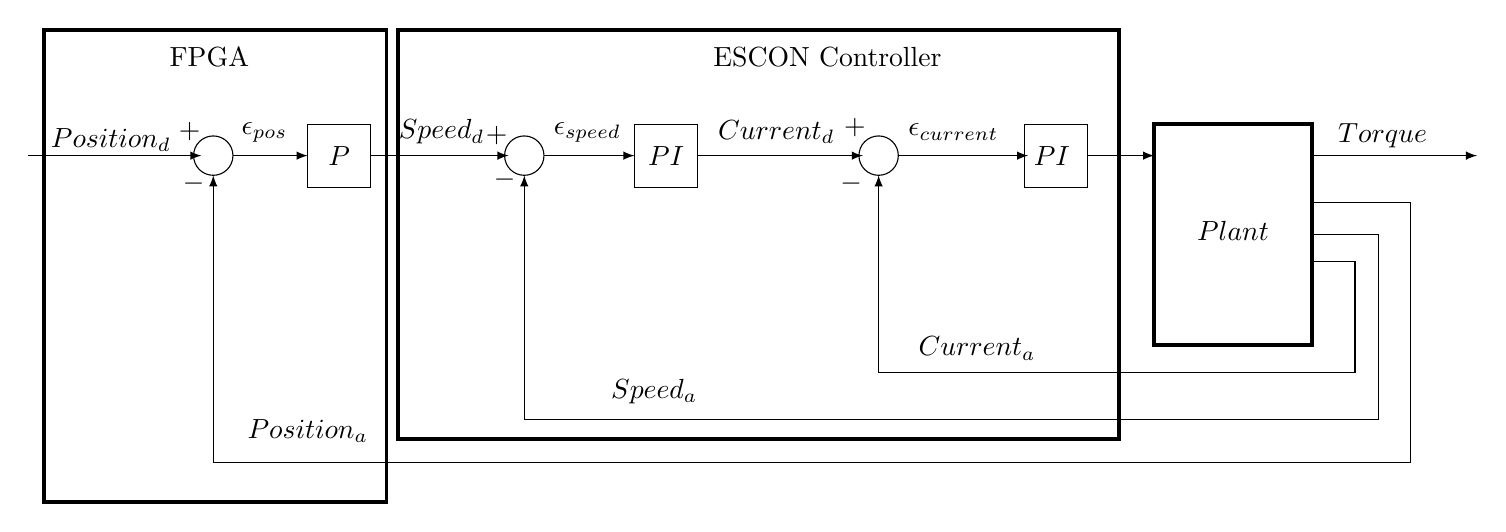
\begin{tikzpicture}%[transform canvas={scale=0.5}]

\draw [-latex] (10.6,3.4) ellipse (0.25 and 0.25);
\node at (7.9,3.4) {\normalsize{$PI$}};
\node at (12.8,3.4) {\normalsize{$PI$}};
\node at (17,3.65) {\normalsize{$Torque$}};
\node at (15.1,2.45) {\normalsize{$Plant$}};
\draw [-latex] (7.5,3.8) rectangle (8.3,3);
\draw [-latex] (12.45,3.8) rectangle (13.25,3);
\draw [-latex](8.3,3.4) -- (10.4,3.4);
\draw [-latex] (6.1,3.4) ellipse (0.25 and 0.25);
\draw [-latex](6.35,3.4) -- (7.5,3.4);
\node at (6.9,3.7) {$\epsilon_{speed}$};
\node at (11.55,3.7) {$\epsilon_{current}$};
\node at (3.75,3.4) {\normalsize{$P$}};
\draw [-latex] (3.35,3.8) rectangle (4.15,3);
\draw [-latex](4.15,3.4) -- (5.9,3.4);

\draw [-latex](10.85,3.4) -- (12.5,3.4);
\draw [-latex](13.25,3.4) -- (14.1,3.4);
\draw [-latex](16.1,3.4) -- (18.2,3.4);

\draw [-latex](16.1,2.05) -- (16.65,2.05) -- (16.65,0.65)-- (10.6,0.65)-- (10.6,3.15);
\draw [-latex](16.1,2.4) -- (16.95,2.4) -- (16.95,0.05)-- (6.1,0.05)-- (6.1,3.15);
\draw [-latex](16.1,2.8) -- (17.35,2.8) -- (17.35,-0.5)-- (2.15,-0.5)-- (2.15,3.15);

\node at (10.3,3.75) {$+$};
\node at (10.25,3.05) {$-$};

\draw [-latex] (2.15,3.4) ellipse (0.25 and 0.25);
\draw [-latex](2.4,3.4) -- (3.35,3.4);
\node at (5.85,3.1) {$-$};

\draw [-latex](-0.2,3.4) -- (2,3.4);
\node at (0.85,3.6) {$Position_d$};
\node at (2.1,4.65) {FPGA};
\node at (9.95,4.65) {ESCON Controller};
\node at (1.9,3.05) {$-$};
\node at (2.8,3.7) {$\epsilon_{pos}$};
\node at (5.05,3.7) {$Speed_d$};
\node at (9.3,3.7) {$Current_d$};
\node at (11.85,0.95) {$Current_a$};
\node at (7.75,0.4) {$Speed_a$};
\node at (3.35,-0.1) {$Position_a$};


\node (v2) at (1.85,3.7) {$+$};
\node (v2) at (5.75,3.65) {$+$};
\draw  [line width=0.5mm](14.1,3.8) rectangle (16.1,1);
\draw  [line width=0.5mm](0,5) rectangle (4.35,-1);
\draw [line width=0.5mm] (4.5,5) rectangle (13.65,-0.2);
\end{tikzpicture}
}
\caption{Embedded cascade control structure. d index means the desired control value, a index means actual value, $\epsilon$ is the error}
\label{cascade_fig}
\end{figure}


It is imperative to create a controller which minimizes the effects of communication delay. Therefore the aim was to implement as much of the motion control on the embedded system as possible. The human operator  inputs the required position by moving the GT. These positions are sent as position reference to the sbRIO. 
The sbRIO has an implemented cascade position-speed-current control, see \figref{cascade_fig}, which takes care of the EndoWrist positioning tasks. The P position control that tracks the setpoint is running on the sbRIO FPGA. The FPGA sends the speed reference to the Escon controller in the form of PWM signals. The Escon controller is running the PI speed control with inner PI current control loop. The inner loops are faster than the outer loops.

The chosen controller parameters:

\begin{center}
	\begin{tabular}{ c | c | c | c }
		\hline
		Controller type & P gain & I time constant & Sampling rate \\ \hline
		Position controller & 10 & $\emptyset$ & 2 kHz \\ \hline
		Speed controller & 426 & 28 ms & 5.36 kHz \\ \hline
		Position controller & 1121 & $38 \mu s$ & 53.6 kHz \\ \hline
	\end{tabular}
\end{center}

The speed and current controller parameters were calibrated automatically by ESCON Studio. The program queries the motor parameters, desired current limits and maximum acceleration values and calculates the controller parameters based on those. The EndoWrist can not handle high speeds and high acceleration, thus speed was not the main priority in tuning the position PID control. We focused on precision and avoiding overshoot. By running experiments, we decided upon a P controller of 10 for each motor. A lower gain would result in slower motion, a higher gain would result in overshoots. The EndoWrist-motor system has inherent damping in the form of friction, inertia and elasticity, thus the system is stable even without integral and differential controller. For the experiments with free-running EndoWrist, see \figref{square_excite}. The setpoints square signals moving jumping between the limits the EndoWrist can move between. This is a movement that would never happen in normal operation. The delay defined in these graphs is the time it takes for the positions to reach the setpoints with an error of 5\%.

%% This file was created by matlab2tikz.
%
%The latest updates can be retrieved from
%  http://www.mathworks.com/matlabcentral/fileexchange/22022-matlab2tikz-matlab2tikz
%where you can also make suggestions and rate matlab2tikz.
%
\definecolor{mycolor1}{rgb}{0.00000,0.44700,0.74100}%
\definecolor{mycolor2}{rgb}{0.85000,0.32500,0.09800}%
%
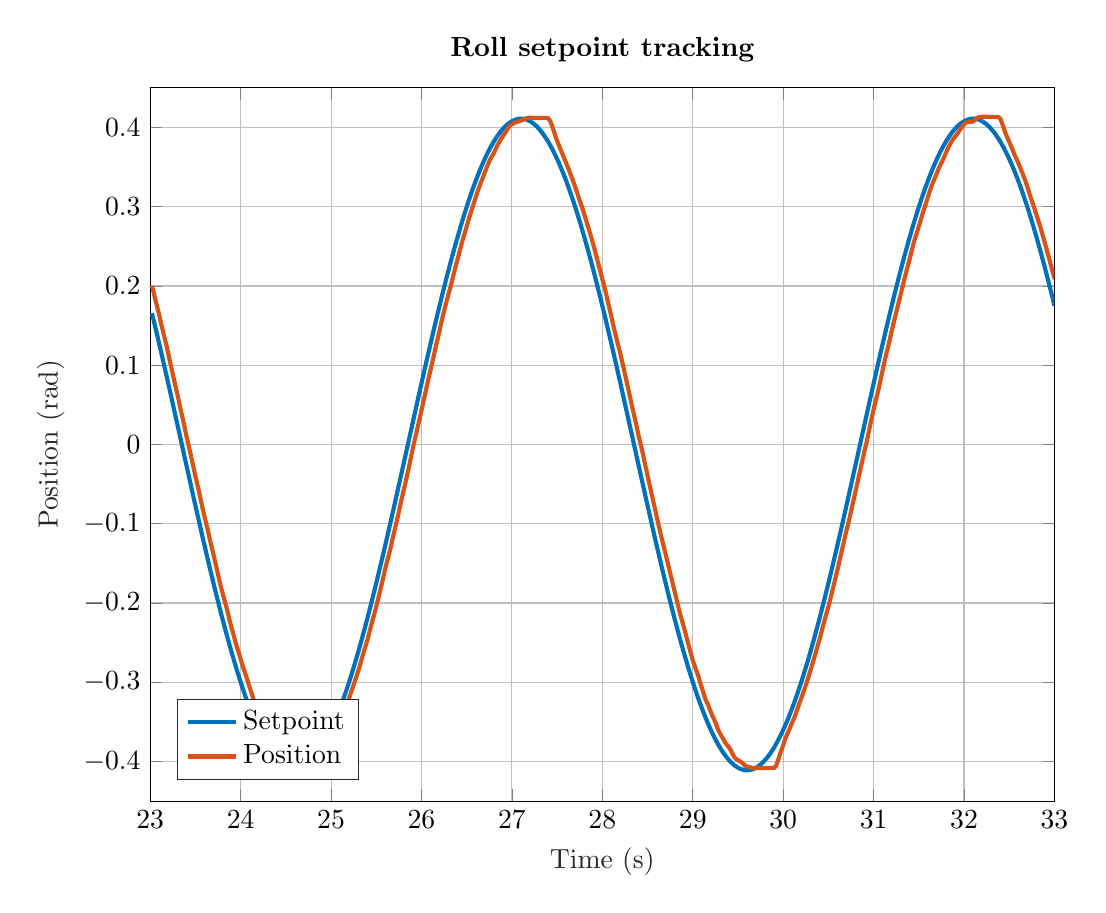
\begin{tikzpicture}

\begin{axis}[%
width=4.521in,
height=3.566in,
at={(0.758in,0.481in)},
scale only axis,
xmin=23,
xmax=33,
xlabel style={font=\color{white!15!black}},
xlabel={Time (s)},
ymin=-0.45,
ymax=0.45,
ylabel style={font=\color{white!15!black}},
ylabel={Position (rad)},
axis background/.style={fill=white},
title style={font=\bfseries},
title={Roll setpoint tracking},
xmajorgrids,
ymajorgrids,
legend style={at={(0.03,0.03)}, anchor=south west, legend cell align=left, align=left, draw=white!15!black}
]
\addplot [color=mycolor1, line width=1.5pt]
  table[row sep=crcr]{%
23.0191555	0.165668769531251\\
23.0791626	0.136850136718749\\
23.11917114	0.117195410156249\\
23.19929695	0.0770482421875016\\
23.3391819	0.00516695312499849\\
23.47919846	-0.0668738281249972\\
23.57920647	-0.117195410156249\\
23.65921402	-0.15615916015625\\
23.71923447	-0.1843680859375\\
23.77923203	-0.211529414062497\\
23.83923912	-0.237488769531247\\
23.87924385	-0.254054121093752\\
23.93925476	-0.277686171874997\\
23.9792614	-0.292572246093748\\
24.01925659	-0.306719218749997\\
24.05926514	-0.32009140625\\
24.09938622	-0.332655000000003\\
24.1392746	-0.344378320312501\\
24.17927551	-0.35523166015625\\
24.21928978	-0.36518767578125\\
24.25928879	-0.374221191406249\\
24.2994175	-0.382309394531248\\
24.33930206	-0.38943185546875\\
24.37930679	-0.395570585937499\\
24.41931152	-0.400710058593752\\
24.45931435	-0.404837304687497\\
24.49943924	-0.407941894531248\\
24.53932953	-0.410015976562498\\
24.57933235	-0.41105435546875\\
24.61933899	-0.41105435546875\\
24.65933609	-0.410015976562498\\
24.69947052	-0.407941894531248\\
24.73935127	-0.404837304687497\\
24.77935219	-0.400710058593752\\
24.81936455	-0.395570585937499\\
24.85939026	-0.38943185546875\\
24.89950562	-0.382309394531248\\
24.93938637	-0.374221191406249\\
24.97940445	-0.36518767578125\\
25.01939392	-0.35523166015625\\
25.05941391	-0.344378320312501\\
25.09952736	-0.332655000000003\\
25.13941765	-0.32009140625\\
25.17942429	-0.306719218749997\\
25.21941948	-0.292572246093748\\
25.2595253	-0.277686171874997\\
25.29954147	-0.262098671875002\\
25.33945274	-0.245849082031249\\
25.37944412	-0.228978476562503\\
25.41944885	-0.211529414062497\\
25.45945358	-0.193546015625003\\
25.51947403	-0.165668769531251\\
25.57947159	-0.136850136718749\\
25.61948204	-0.117195410156249\\
25.69965935	-0.0770482421875016\\
25.89969635	0.0258184765624989\\
25.95955086	0.0566571875000008\\
26.03957939	0.0972446484375027\\
26.09970474	0.127062910156248\\
26.13957214	0.146550937500002\\
26.17958832	0.165668769531251\\
26.23957825	0.193546015625003\\
26.27958679	0.211529414062497\\
26.33958435	0.237488769531247\\
26.37959862	0.254054121093752\\
26.43959999	0.277686171874997\\
26.47961998	0.292572246093748\\
26.51965904	0.306719218749997\\
26.559618	0.32009140625\\
26.59978867	0.332655000000003\\
26.63961983	0.344378320312501\\
26.67969131	0.35523166015625\\
26.71968079	0.36518767578125\\
26.7596817	0.374221191406249\\
26.79981041	0.382309394531248\\
26.83969688	0.38943185546875\\
26.8796978	0.395570585937499\\
26.91968918	0.400710058593752\\
26.95970345	0.404837304687497\\
26.9998188	0.407941894531248\\
27.03972244	0.410015976562498\\
27.07970428	0.41105435546875\\
27.11972046	0.41105435546875\\
27.15972137	0.410015976562498\\
27.19987488	0.407941894531248\\
27.23973846	0.404837304687497\\
27.27972794	0.400710058593752\\
27.31974983	0.395570585937499\\
27.3597641	0.38943185546875\\
27.39987946	0.382309394531248\\
27.43976212	0.374221191406249\\
27.47976685	0.36518767578125\\
27.51978683	0.35523166015625\\
27.55976677	0.344378320312501\\
27.59990501	0.332655000000003\\
27.63977814	0.32009140625\\
27.67980003	0.306719218749997\\
27.71977997	0.292572246093748\\
27.75979042	0.277686171874997\\
27.79992867	0.262098671875002\\
27.83981323	0.245849082031249\\
27.87981415	0.228978476562503\\
27.91983032	0.211529414062497\\
27.97982025	0.1843680859375\\
28.01981544	0.165668769531251\\
28.07985115	0.136850136718749\\
28.11987686	0.117195410156249\\
28.19997215	0.0770482421875016\\
28.31985855	0.0154976171874992\\
28.47991753	-0.0668738281249972\\
28.57987976	-0.117195410156249\\
28.65989304	-0.15615916015625\\
28.71993256	-0.1843680859375\\
28.75995255	-0.202601699218746\\
28.80004501	-0.220323515624997\\
28.8399334	-0.237488769531247\\
28.87992287	-0.254054121093752\\
28.93993759	-0.277686171874997\\
28.97994614	-0.292572246093748\\
29.01994705	-0.306719218749997\\
29.05997849	-0.32009140625\\
29.10009575	-0.332655000000003\\
29.13996696	-0.344378320312501\\
29.17998505	-0.35523166015625\\
29.21994209	-0.36518767578125\\
29.25997353	-0.374221191406249\\
29.30012321	-0.382309394531248\\
29.34000587	-0.38943185546875\\
29.3800087	-0.395570585937499\\
29.41999435	-0.400710058593752\\
29.46001816	-0.404837304687497\\
29.50014114	-0.407941894531248\\
29.54003143	-0.410015976562498\\
29.58001518	-0.41105435546875\\
29.62005615	-0.41105435546875\\
29.66002274	-0.410015976562498\\
29.70015717	-0.407941894531248\\
29.74006462	-0.404837304687497\\
29.78003311	-0.400710058593752\\
29.82004356	-0.395570585937499\\
29.86007118	-0.38943185546875\\
29.90019608	-0.382309394531248\\
29.94006538	-0.374221191406249\\
29.98004532	-0.36518767578125\\
30.02007484	-0.35523166015625\\
30.06008911	-0.344378320312501\\
30.10021591	-0.332655000000003\\
30.14009857	-0.32009140625\\
30.18009949	-0.306719218749997\\
30.22017097	-0.292572246093748\\
30.26011658	-0.277686171874997\\
30.30026627	-0.262098671875002\\
30.34012604	-0.245849082031249\\
30.40029907	-0.220323515624997\\
30.4601326	-0.193546015625003\\
30.52017593	-0.165668769531251\\
30.58013344	-0.136850136718749\\
30.62013245	-0.117195410156249\\
30.70029259	-0.0770482421875016\\
30.84021378	-0.00516695312499849\\
30.980196	0.0668738281249972\\
31.08020401	0.117195410156249\\
31.1602459	0.15615916015625\\
31.22019577	0.1843680859375\\
31.28022957	0.211529414062497\\
31.34022331	0.237488769531247\\
31.38021278	0.254054121093752\\
31.44024277	0.277686171874997\\
31.48025322	0.292572246093748\\
31.520298	0.306719218749997\\
31.56042099	0.32009140625\\
31.60041428	0.332655000000003\\
31.64028549	0.344378320312501\\
31.68028259	0.35523166015625\\
31.72029877	0.36518767578125\\
31.76030731	0.374221191406249\\
31.80044556	0.382309394531248\\
31.84035492	0.38943185546875\\
31.88029289	0.395570585937499\\
31.92034912	0.400710058593752\\
31.96029282	0.404837304687497\\
32.00043488	0.407941894531248\\
32.04032898	0.410015976562498\\
32.08035278	0.41105435546875\\
32.12031555	0.41105435546875\\
32.16034317	0.410015976562498\\
32.20049286	0.407941894531248\\
32.24038315	0.404837304687497\\
32.28037262	0.400710058593752\\
32.32038116	0.395570585937499\\
32.36040878	0.38943185546875\\
32.40048218	0.382309394531248\\
32.44039536	0.374221191406249\\
32.48039627	0.36518767578125\\
32.5204277	0.35523166015625\\
32.56040192	0.344378320312501\\
32.60052109	0.332655000000003\\
32.64037704	0.32009140625\\
32.68041992	0.306719218749997\\
32.72045135	0.292572246093748\\
32.7604332	0.277686171874997\\
32.8005867	0.262098671875002\\
32.86040115	0.237488769531247\\
32.90053558	0.220323515624997\\
32.96042633	0.193546015625003\\
33.00058746	0.175073710937497\\
};
\addlegendentry{Setpoint}

\addplot [color=mycolor2, line width=1.5pt]
  table[row sep=crcr]{%
23.0191555	0.200063183593748\\
23.03915405	0.191505195312502\\
23.05915833	0.181332500000003\\
23.0992794	0.163247695312499\\
23.11917114	0.153074980468752\\
23.15916443	0.134182812500001\\
23.17917252	0.125140410156249\\
23.19929695	0.114806230468751\\
23.21917725	0.104149121093748\\
23.27918243	0.0737924804687466\\
23.29930305	0.0639427148437477\\
23.31919098	0.0529626562500027\\
23.3391819	0.0426284765624985\\
23.35918236	0.0327787109374995\\
23.37919235	0.0222830664062528\\
23.39931488	0.0111415234375016\\
23.41919327	0.00161470703125133\\
23.43920135	-0.00839652343749719\\
23.4993248	-0.0398834570312516\\
23.53920555	-0.0595829882812495\\
23.57920647	-0.0807357421874997\\
23.63921356	-0.1093162109375\\
23.65921402	-0.119650371093748\\
23.69934082	-0.138865488281247\\
23.77923203	-0.178748945312499\\
23.83923912	-0.203777031249999\\
23.87924385	-0.222507714843751\\
23.89936638	-0.231227187499996\\
23.91924667	-0.239462226562502\\
23.93925476	-0.248181699218748\\
23.95925522	-0.255770859374998\\
23.9792614	-0.26287560546875\\
24.01925659	-0.278215390625\\
24.05926514	-0.291940468749999\\
24.1392746	-0.32052091796875\\
24.21928978	-0.343934277343749\\
24.23929024	-0.34910138671875\\
24.25928879	-0.354914375\\
24.27929878	-0.361211738281249\\
24.2994175	-0.364925605468748\\
24.33930206	-0.374129453125001\\
24.35929871	-0.377843300781251\\
24.39942551	-0.383979238281249\\
24.4393177	-0.39156837890625\\
24.45931435	-0.394636367187502\\
24.47932053	-0.396896933593752\\
24.53932953	-0.399641953124998\\
24.55933571	-0.402225507812503\\
24.57933235	-0.405293457031249\\
24.59946823	-0.4069081640625\\
24.61933899	-0.407876992187497\\
24.67933464	-0.408038476562503\\
24.87937546	-0.407715527343747\\
24.89950562	-0.407554062499997\\
24.9193821	-0.404001679687497\\
24.9593811	-0.392214277343747\\
24.99950981	-0.379296582031252\\
25.03940964	-0.367024707031248\\
25.05941391	-0.362180546875003\\
25.07941818	-0.356851992187501\\
25.11941338	-0.345064589843751\\
25.13941765	-0.338282792968748\\
25.15943146	-0.332469824218748\\
25.17942429	-0.326172421875\\
25.19954681	-0.320197988281251\\
25.21941948	-0.313093222656249\\
25.23942566	-0.306795839843751\\
25.27942657	-0.293232246093751\\
25.31944466	-0.278861289062498\\
25.33945274	-0.270303281250001\\
25.37944412	-0.254963496093751\\
25.39957237	-0.2475358203125\\
25.41944885	-0.238977812500003\\
25.43946648	-0.229773945312502\\
25.47947884	-0.213465312499999\\
25.49957657	-0.204584394531253\\
25.55951691	-0.17648833984375\\
25.57947159	-0.166800058593751\\
25.59960938	-0.156465878906253\\
25.61948204	-0.147423476562501\\
25.63947678	-0.139349902343753\\
25.65950775	-0.129984570312502\\
25.67949295	-0.119327421874999\\
25.71951675	-0.100112324218749\\
25.7395134	-0.0904240429687491\\
25.77954102	-0.0691098046874998\\
25.81952286	-0.0498946875000001\\
25.83953857	-0.0392375781249967\\
25.85951996	-0.0295492773437473\\
25.89969635	-0.00710474609375211\\
25.97954559	0.0327787109374995\\
26.07955933	0.0841266601562509\\
26.11956024	0.1035032421875\\
26.13957214	0.113998886718747\\
26.17958832	0.133536933593753\\
26.19974518	0.143709628906251\\
26.21959496	0.154366757812497\\
26.23957825	0.163893574218747\\
26.29973793	0.190536367187498\\
26.31958199	0.198125527343748\\
26.37959862	0.225737148437503\\
26.39978218	0.234133671875\\
26.43959999	0.251572617187499\\
26.45960236	0.259969121093754\\
26.47961998	0.267235332031248\\
26.49975395	0.274985937499999\\
26.51965904	0.283059550781253\\
26.53966522	0.290648691406247\\
26.61962128	0.318906191406249\\
26.65966988	0.331500976562502\\
26.67969131	0.336829550781253\\
26.69979858	0.342803984375003\\
26.71968079	0.3492628515625\\
26.7596817	0.359758496093747\\
26.77966881	0.363795292968753\\
26.79981041	0.367509121093747\\
26.81968689	0.372676230468748\\
26.83969688	0.377520371093752\\
26.8796978	0.3855939453125\\
26.91968918	0.392214277343747\\
26.95970345	0.399641953124998\\
26.97970009	0.402548437500002\\
27.01970673	0.405293457031249\\
27.05970955	0.407231132812498\\
27.07970428	0.407715527343747\\
27.09983826	0.40884583984375\\
27.11972046	0.409330234374998\\
27.1397171	0.410299082031251\\
27.15972137	0.411752324218753\\
27.17972946	0.412236757812501\\
27.37975121	0.412075234375003\\
27.39987946	0.411752324218753\\
27.41974258	0.408684375\\
27.43976212	0.403355800781249\\
27.45976257	0.396896933593752\\
27.47976685	0.389469238281251\\
27.49986458	0.383010390625003\\
27.57977867	0.360565839843751\\
27.59990501	0.35523728515625\\
27.63977814	0.34361134765625\\
27.67980003	0.331662441406252\\
27.71977997	0.318260312500001\\
27.73979187	0.311155566406249\\
27.77978325	0.298076406249997\\
27.87981415	0.260453535156252\\
27.89992714	0.252379941406247\\
27.93980408	0.235263964843753\\
27.99995804	0.208459687500003\\
28.01981544	0.200224667968747\\
28.03981781	0.191343730468752\\
28.05982971	0.181009550781248\\
28.09995842	0.16131001953125\\
28.11987686	0.151137304687502\\
28.13983154	0.141449023437502\\
28.19997215	0.113998886718747\\
28.23985672	0.0941378906249994\\
28.27983856	0.073469531249998\\
28.3000145	0.0634583007812495\\
28.31985855	0.052639707031247\\
28.37986183	0.022767480468751\\
28.40002632	0.0114644726562503\\
28.41988564	0.00226060546874862\\
28.43987274	-0.00742769531250076\\
28.45988464	-0.0184077539062528\\
28.51988983	-0.049571757812501\\
28.57987976	-0.080251347656251\\
28.61990929	-0.100596738281247\\
28.65989304	-0.119973320312504\\
28.67989922	-0.129015722656249\\
28.8399334	-0.204584394531253\\
28.85992241	-0.213626796874998\\
28.91993523	-0.23817044921875\\
28.93993759	-0.247374316406251\\
29.00005722	-0.272402421875\\
29.01994705	-0.279184199218747\\
29.05997849	-0.29177900390625\\
29.0799942	-0.299691113281249\\
29.13996696	-0.321489765625003\\
29.15997696	-0.32633388671875\\
29.17998505	-0.331662441406252\\
29.20013809	-0.33779837890625\\
29.21994209	-0.343126933593751\\
29.23999405	-0.347809609374998\\
29.25997353	-0.353622578124998\\
29.27997208	-0.359919960937503\\
29.30012321	-0.36444119140625\\
29.34000587	-0.372191796875001\\
29.36000061	-0.376551523437499\\
29.3800087	-0.379619472656252\\
29.40013885	-0.38188009765625\\
29.41999435	-0.385916874999999\\
29.46001816	-0.394797792968753\\
29.48002243	-0.3970584375\\
29.5200119	-0.399641953124998\\
29.54003143	-0.4010951953125\\
29.58001518	-0.405454921874998\\
29.60014915	-0.406423750000002\\
29.62005615	-0.406746699218751\\
29.66002274	-0.408361425781251\\
29.90019608	-0.408038476562503\\
29.92011642	-0.405939355468753\\
29.94006538	-0.399480488281249\\
29.98004532	-0.38575541015625\\
30.00018692	-0.379296582031252\\
30.02007484	-0.372514746093749\\
30.0401001	-0.366701777343749\\
30.06008911	-0.361857617187503\\
30.08009148	-0.356044648437504\\
30.12007904	-0.345710468749999\\
30.14009857	-0.33973603515625\\
30.18009949	-0.326010957031251\\
30.20022011	-0.320359453125\\
30.26011658	-0.300498437500003\\
30.32013321	-0.27837685546875\\
30.34012604	-0.270303281250001\\
30.36011124	-0.262714140625\\
30.38015175	-0.254479082031253\\
30.40029907	-0.246728457031253\\
30.42012215	-0.238331933593749\\
30.44019699	-0.229128046874997\\
30.50025749	-0.204422910156246\\
30.52017593	-0.19570345703125\\
30.60030365	-0.158242070312497\\
30.62013245	-0.148069355468749\\
30.70029259	-0.108347363281247\\
30.7202034	-0.0994664453125012\\
30.74013329	-0.0897781640625013\\
30.80030251	-0.0589370898437522\\
30.82019997	-0.0489258593749966\\
30.84021378	-0.0381072656250012\\
30.8602047	-0.0284189843750013\\
30.90029144	-0.00758916015625033\\
30.92017746	0.00161470703125133\\
30.94021988	0.0122718359374971\\
30.96017838	0.0234133593749988\\
31.00031853	0.0445661328124984\\
31.02017975	0.0539314843749992\\
31.04024887	0.0626509375000026\\
31.06018448	0.072339238281252\\
31.10031509	0.0941378906249994\\
31.14019394	0.114321816406253\\
31.1602459	0.123202753906249\\
31.20035934	0.143225214843753\\
31.22019577	0.152752031250003\\
31.32023621	0.198932871093753\\
31.34022331	0.208459687500003\\
31.38021278	0.226221562500001\\
31.40035629	0.234779550781248\\
31.42024994	0.24366048828125\\
31.44024277	0.253025820312502\\
31.46025085	0.260776464843751\\
31.48025322	0.267719765625003\\
31.50040054	0.275631835937503\\
31.54026985	0.290648691406247\\
31.5802803	0.304696699218752\\
31.60041428	0.312285878906252\\
31.62028503	0.319390644531254\\
31.64028549	0.325849492187501\\
31.66029358	0.331662441406252\\
31.70036697	0.342319570312497\\
31.72029877	0.348294042968753\\
31.74024773	0.35329962890625\\
31.76030731	0.357659355468748\\
31.78029251	0.362987929687499\\
31.80044556	0.367993554687502\\
31.82031822	0.373322109375003\\
31.8602562	0.3820415625\\
31.88029289	0.3855939453125\\
31.90040207	0.388177480468748\\
31.94027901	0.394313398437497\\
31.96029282	0.398188710937497\\
31.98027229	0.401256699218749\\
32.02036285	0.406100800781253\\
32.04032898	0.406746699218751\\
32.08035278	0.4069081640625\\
32.10045242	0.407715527343747\\
32.12031555	0.409330234374998\\
32.14030457	0.411752324218753\\
32.16034317	0.41288259765625\\
32.20049286	0.413528496093747\\
32.36040878	0.413367031249997\\
32.38039017	0.413044121093748\\
32.40048218	0.411267890624998\\
32.42037964	0.405616386718748\\
32.46037674	0.392214277343747\\
32.54035187	0.371222968749997\\
32.56040192	0.365248535156248\\
32.60052109	0.35523728515625\\
32.64037704	0.343934277343749\\
32.68041992	0.331985390625\\
32.70054245	0.325203613281253\\
32.74040604	0.310671171875001\\
32.78042221	0.297269023437501\\
32.84041977	0.275793320312502\\
32.90053558	0.251734082031248\\
32.98042679	0.217825058593753\\
33.00058746	0.208782636718752\\
};
\addlegendentry{Position}

\end{axis}
\end{tikzpicture}%




\begin{figure}
	\begin{subfigure}[b]{0.5\textwidth}
		\centering
		\resizebox{\linewidth}{!}{
			% This file was created by matlab2tikz.
%
%The latest updates can be retrieved from
%  http://www.mathworks.com/matlabcentral/fileexchange/22022-matlab2tikz-matlab2tikz
%where you can also make suggestions and rate matlab2tikz.
%
\definecolor{mycolor1}{rgb}{0.00000,0.44700,0.74100}%
\definecolor{mycolor2}{rgb}{0.85000,0.32500,0.09800}%
%
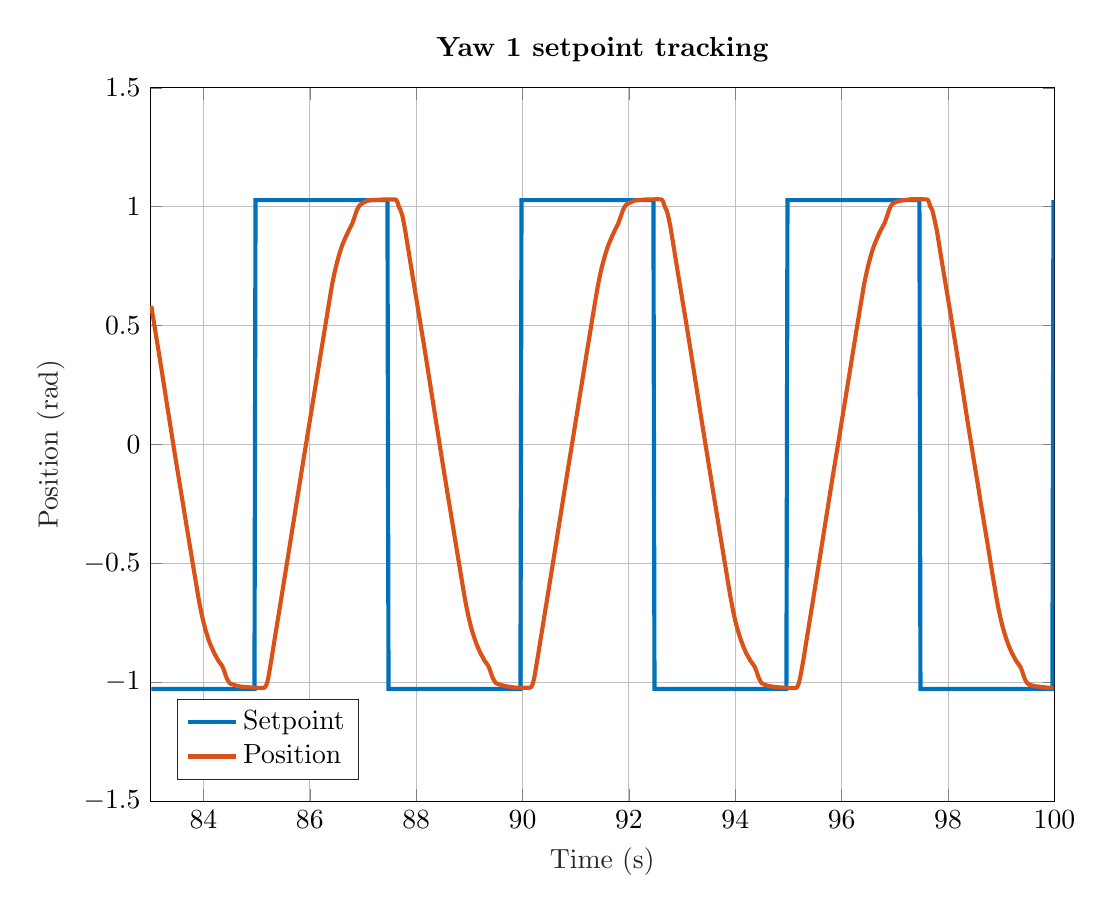
\begin{tikzpicture}

\begin{axis}[%
width=4.521in,
height=3.566in,
at={(0.758in,0.481in)},
scale only axis,
xmin=83,
xmax=100,
xlabel style={font=\color{white!15!black}},
xlabel={Time (s)},
ymin=-1.5,
ymax=1.5,
ylabel style={font=\color{white!15!black}},
ylabel={Position (rad)},
axis background/.style={fill=white},
title style={font=\bfseries},
title={Yaw 1 setpoint tracking},
xmajorgrids,
ymajorgrids,
legend style={at={(0.03,0.03)}, anchor=south west, legend cell align=left, align=left, draw=white!15!black}
]
\addplot [color=mycolor1, line width=1.5pt]
  table[row sep=crcr]{%
83.01917267	-1.02796056640625\\
84.95939636	-1.02796056640625\\
84.97940063	1.02796056640625\\
87.45979309	1.02796056640625\\
87.47977448	-1.02796056640625\\
89.96006775	-1.02796056640625\\
89.98009491	1.02796056640625\\
92.46042633	1.02796056640625\\
92.4803772	-1.02796056640625\\
94.96068573	-1.02796056640625\\
94.98072052	1.02796056640625\\
97.46098328	1.02796056640625\\
97.48095703	-1.02796056640625\\
99.96131897	-1.02796056640625\\
99.98136902	1.02796056640625\\
};
\addlegendentry{Setpoint}

\addplot [color=mycolor2, line width=1.5pt]
  table[row sep=crcr]{%
83.01917267	0.582912128906244\\
83.21920013	0.305665546875005\\
83.31920624	0.162117363281254\\
83.37921906	0.0771833789062555\\
83.43921661	-0.0077506249999999\\
83.49934387	-0.0913928710937455\\
83.55923462	-0.173097441406256\\
83.79937744	-0.501046074218749\\
83.87928009	-0.608101660156251\\
83.89938354	-0.636197734375003\\
83.93927765	-0.683993281249997\\
83.97928619	-0.726298828124996\\
83.99938965	-0.745675351562497\\
84.03928375	-0.779584394531256\\
84.09941101	-0.823343164062507\\
84.13932037	-0.846433632812506\\
84.21930695	-0.885186718750006\\
84.23931122	-0.892291542968749\\
84.25931549	-0.901333867187503\\
84.29943085	-0.915704882812506\\
84.33931732	-0.927492285156248\\
84.35932922	-0.934919921874993\\
84.37934113	-0.945577109374995\\
84.39944458	-0.958010371093749\\
84.41933441	-0.972058457031252\\
84.43933105	-0.983522851562498\\
84.47933197	-0.999670117187506\\
84.49945068	-1.00419123046875\\
84.51934814	-1.0074205859375\\
84.55934906	-1.009842734375\\
84.59946442	-1.01307220703126\\
84.61935425	-1.01533275390625\\
84.73937225	-1.02001544921875\\
85.05943298	-1.02421361328125\\
85.13943481	-1.023244921875\\
85.15944672	-1.02049986328124\\
85.17941284	-1.01339513671876\\
85.19954681	-1.00047734375001\\
85.21952057	-0.981423769531247\\
85.23944855	-0.957041562499995\\
85.29961395	-0.8750140625\\
85.35948181	-0.790402988281244\\
85.43946838	-0.680925332031251\\
85.47948456	-0.624894687500003\\
85.5194931	-0.569671445312494\\
85.61950684	-0.42999859375\\
85.69962311	-0.317291503906247\\
85.85955048	-0.0936534765624941\\
86.39974976	0.647985136718745\\
86.41962433	0.673336152343751\\
86.45962524	0.717094921875002\\
86.49979401	0.754717792968748\\
86.53964233	0.78878826171875\\
86.55963135	0.804289531250006\\
86.59978485	0.831578222656248\\
86.61964417	0.843850019531246\\
86.6796875	0.875175468750001\\
86.73968506	0.903594472656252\\
86.77967834	0.920710507812501\\
86.79982758	0.930075761718754\\
86.83972168	0.955749765625001\\
86.87970734	0.982554042968744\\
86.89983368	0.99224236328125\\
86.91971588	1.00015441406251\\
86.93975067	1.006613359375\\
86.95972443	1.01048859375\\
87.01973724	1.018239296875\\
87.07971954	1.0251825390625\\
87.13975525	1.02744310546875\\
87.41979218	1.03083404296875\\
87.59990692	1.03051111328125\\
87.61981201	1.0290577734375\\
87.63980103	1.0237293359375\\
87.67980957	0.996763593750003\\
87.69992828	0.989174355468748\\
87.73979187	0.963015957031246\\
87.75980377	0.941217343749997\\
87.7798233	0.917481074218756\\
87.79993439	0.891807031249996\\
87.91982269	0.725975839843755\\
88.07984161	0.508150839843751\\
88.13987732	0.427092128906253\\
88.19998169	0.342481074218753\\
88.50001526	-0.0828348828125058\\
88.5398941	-0.137412246093746\\
88.60003662	-0.220408593749994\\
88.659935	-0.30114435546875\\
88.7199173	-0.383171855468746\\
88.779953	-0.465199414062496\\
88.8399353	-0.547226933593748\\
88.87994385	-0.600835488281248\\
88.90008545	-0.628770039062502\\
88.93996429	-0.677534433593749\\
88.97995758	-0.720162871093748\\
89.01996613	-0.758270156250006\\
89.03997803	-0.775224707031256\\
89.10012054	-0.818499023437496\\
89.13998413	-0.843365625000004\\
89.2000885	-0.873883769531247\\
89.22001648	-0.8827646875\\
89.26000977	-0.898588847656256\\
89.27999878	-0.90763130859375\\
89.33998871	-0.926039003906254\\
89.36000061	-0.933951171874995\\
89.3800354	-0.944769707031256\\
89.40014648	-0.957041562499995\\
89.42004395	-0.970605175781245\\
89.44000244	-0.982231113281244\\
89.48002625	-0.998378261718756\\
89.50016022	-1.00354535156249\\
89.56002045	-1.0093583203125\\
89.68005371	-1.01694744140624\\
89.78005219	-1.0201769140625\\
89.82007599	-1.02163013671876\\
89.86008453	-1.0225989453125\\
90.10025024	-1.02356787109375\\
90.14012146	-1.02292199218751\\
90.16012573	-1.02033837890625\\
90.18012238	-1.01307220703126\\
90.20025635	-0.999670117187506\\
90.22013092	-0.98061642578125\\
90.24012756	-0.956557226562495\\
90.28011322	-0.902141269531256\\
90.46013641	-0.6526677734375\\
90.64015198	-0.402709902343744\\
90.80029297	-0.177295703124997\\
90.88018799	-0.0670106640624937\\
90.92016602	-0.0124333007812538\\
91.18025208	0.348132539062505\\
91.24021912	0.430483027343755\\
91.38025665	0.621826738281257\\
91.42025757	0.672528749999998\\
91.46028137	0.716126054687507\\
91.48025513	0.736310039062502\\
91.52025604	0.771187890625001\\
91.56024933	0.803320722656252\\
91.60038757	0.830770820312495\\
91.62030792	0.842881210937506\\
91.70042419	0.884540839843751\\
91.80041504	0.930398828125007\\
91.86031342	0.9676986328125\\
91.88027954	0.981585234375004\\
91.90042877	0.991596484374995\\
91.92029572	0.999831601562505\\
91.94029999	1.006613359375\\
91.96030426	1.010650078125\\
92.10043335	1.025666953125\\
92.16034698	1.02760457031251\\
92.34037018	1.03083404296875\\
92.54039001	1.0313184375\\
92.60050201	1.03099550781251\\
92.62042999	1.0290577734375\\
92.64041138	1.02308345703125\\
92.68039703	0.996763593750003\\
92.70055389	0.989497285156247\\
92.72039795	0.975449335937498\\
92.74043274	0.958656308593746\\
92.76040649	0.937664999999996\\
92.78044128	0.914574550781253\\
92.82043457	0.860158652343756\\
92.92041779	0.722262011718755\\
93.10058594	0.478278613281248\\
93.16043854	0.393990449218748\\
93.28045654	0.22460685546875\\
93.36048889	0.109800625000005\\
93.50061035	-0.0846110546874996\\
93.54051971	-0.139188437499996\\
93.60061646	-0.222507714843744\\
93.66052246	-0.303889355468755\\
93.70068359	-0.359919960937503\\
93.90073395	-0.631030585937495\\
93.94054413	-0.6793105859375\\
93.98055267	-0.722907890624995\\
94.0007019	-0.742607402343751\\
94.04055786	-0.776839374999994\\
94.10071564	-0.820113750000004\\
94.16056824	-0.855153027343746\\
94.20072174	-0.875659980468754\\
94.22061157	-0.88437943359375\\
94.2605896	-0.899719199218751\\
94.28057861	-0.908600175781245\\
94.36061096	-0.933305195312499\\
94.40074158	-0.955911230468743\\
94.42059326	-0.969636308593749\\
94.44059753	-0.981746699218746\\
94.48060608	-0.999024140624996\\
94.50074768	-1.004837109375\\
94.54064178	-1.00968126953126\\
94.58063507	-1.0125876953125\\
94.62065125	-1.01565570312501\\
94.70081329	-1.01840076171875\\
94.76068115	-1.02033837890625\\
94.82070923	-1.0217916015625\\
94.94071198	-1.02308345703125\\
94.98072052	-1.024859609375\\
95.14070892	-1.02389080078125\\
95.16072083	-1.02049986328124\\
95.18074036	-1.0125876953125\\
95.20083618	-0.998378261718756\\
95.22074127	-0.978678808593756\\
95.24073792	-0.955426894531243\\
95.28071594	-0.904886230468748\\
95.34075928	-0.821405546874999\\
95.48073578	-0.627316757812494\\
95.64076233	-0.403678749999997\\
95.82080841	-0.149361132812501\\
95.94082642	0.0142094921875042\\
96.00091553	0.097367304687495\\
96.06082153	0.179394824218747\\
96.28082275	0.484575957031254\\
96.34082794	0.56595763671875\\
96.40099335	0.647500683593748\\
96.42087555	0.673013222656252\\
96.44083405	0.695296269531255\\
96.48086548	0.735987089843746\\
96.50099182	0.754717792968748\\
96.56088257	0.804450996093749\\
96.60098267	0.831901152343747\\
96.62090302	0.844011484375002\\
96.70102692	0.885671171875003\\
96.74092865	0.903917480468749\\
96.80101776	0.928461152343743\\
96.82090759	0.939764082031246\\
96.86090088	0.965922480468748\\
96.88088989	0.979647499999999\\
96.90106201	0.991596484374995\\
96.92089844	1.00112322265625\\
96.94093323	1.008228046875\\
96.96091461	1.01339513671876\\
97.00104523	1.01840076171875\\
97.0409317	1.02195306640625\\
97.16094971	1.02776615234374\\
97.30109406	1.0313184375\\
97.48095703	1.03164138671875\\
97.60108948	1.03083404296875\\
97.62100983	1.02776615234374\\
97.64096069	1.01872371093749\\
97.66101074	1.00306095703125\\
97.70115662	0.987236738281254\\
97.72100067	0.970605175781245\\
97.78102112	0.909084570312501\\
97.80110168	0.883733437499998\\
97.88104248	0.771995234374998\\
98.02106476	0.5833965234375\\
98.10118103	0.474241796875006\\
98.16103363	0.390761015625003\\
98.28103638	0.220408593749994\\
98.36109924	0.104633535156253\\
98.48110199	-0.0615206445312566\\
98.56111145	-0.170675390624993\\
98.60124207	-0.227028925781255\\
98.76113892	-0.443885156250005\\
98.84115601	-0.553685761718754\\
98.90132904	-0.634098593749997\\
98.94119263	-0.683185878906244\\
98.98121643	-0.725168496093744\\
99.02119446	-0.762952832031246\\
99.061203	-0.793955351562502\\
99.10132599	-0.822212890624996\\
99.14120483	-0.846595039062507\\
99.20133209	-0.877920546875004\\
99.28121948	-0.910699257812496\\
99.36122131	-0.935888789062503\\
99.38127136	-0.946868906250003\\
99.40136719	-0.959625058593744\\
99.42127991	-0.974480468750002\\
99.44121552	-0.985137656250004\\
99.46130371	-0.994502910156257\\
99.48130035	-1.00176921875\\
99.52122498	-1.009842734375\\
99.62133789	-1.01646314453124\\
99.82130432	-1.0217916015625\\
99.90144348	-1.02340638671875\\
99.96131897	-1.0243751953125\\
99.98136902	-1.0243751953125\\
};
\addlegendentry{Position}

\end{axis}
\end{tikzpicture}%
		}
		\caption{Yaw 1 delay is 1.7 s}
	\end{subfigure}
	\begin{subfigure}[b]{0.5\textwidth}
		\centering
		\resizebox{\linewidth}{!}{
			% This file was created by matlab2tikz.
%
%The latest updates can be retrieved from
%  http://www.mathworks.com/matlabcentral/fileexchange/22022-matlab2tikz-matlab2tikz
%where you can also make suggestions and rate matlab2tikz.
%
\definecolor{mycolor1}{rgb}{0.00000,0.44700,0.74100}%
\definecolor{mycolor2}{rgb}{0.85000,0.32500,0.09800}%
%
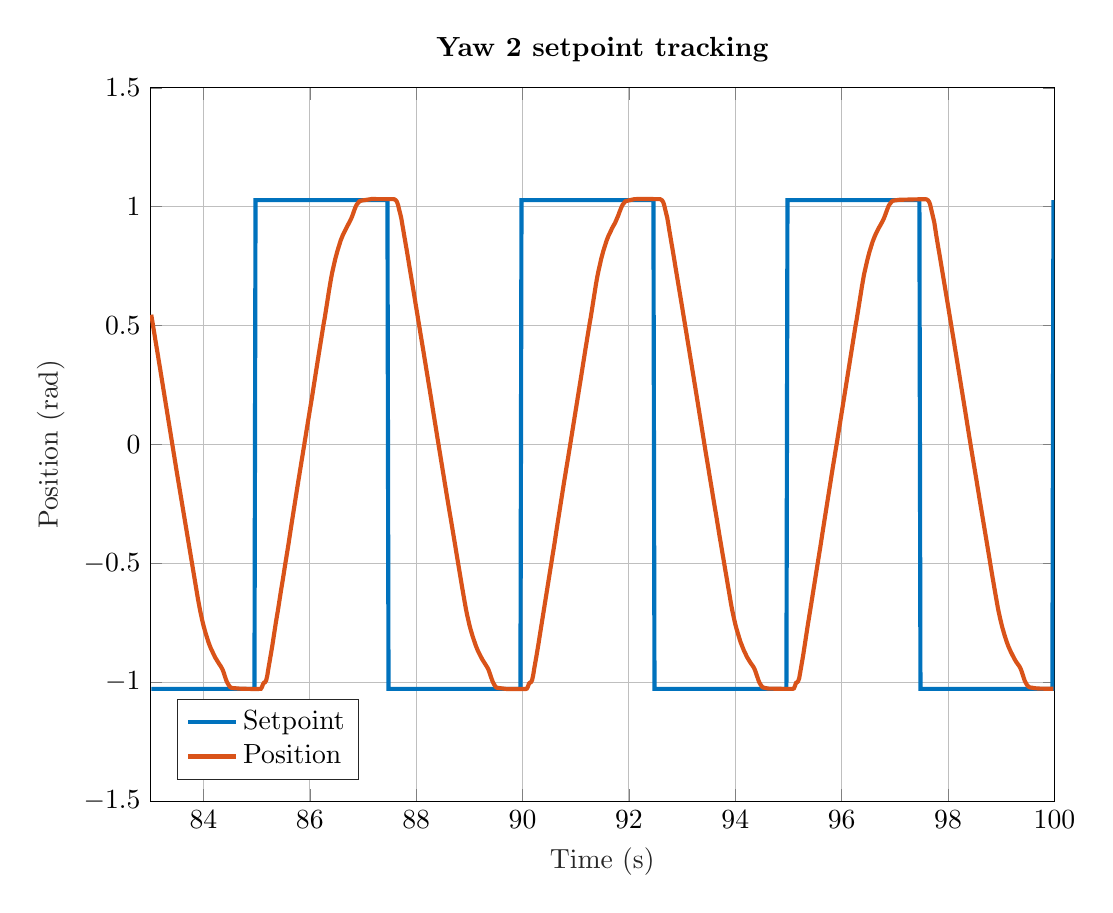
\begin{tikzpicture}

\begin{axis}[%
width=4.521in,
height=3.566in,
at={(0.758in,0.481in)},
scale only axis,
xmin=83,
xmax=100,
xlabel style={font=\color{white!15!black}},
xlabel={Time (s)},
ymin=-1.5,
ymax=1.5,
ylabel style={font=\color{white!15!black}},
ylabel={Position (rad)},
axis background/.style={fill=white},
title style={font=\bfseries},
title={Yaw 2 setpoint tracking},
xmajorgrids,
ymajorgrids,
legend style={at={(0.03,0.03)}, anchor=south west, legend cell align=left, align=left, draw=white!15!black}
]
\addplot [color=mycolor1, line width=1.5pt]
  table[row sep=crcr]{%
83.01917267	-1.02796056640625\\
84.95939636	-1.02796056640625\\
84.97940063	1.02796056640625\\
87.45979309	1.02796056640625\\
87.47977448	-1.02796056640625\\
89.96006775	-1.02796056640625\\
89.98009491	1.02796056640625\\
92.46042633	1.02796056640625\\
92.4803772	-1.02796056640625\\
94.96068573	-1.02796056640625\\
94.98072052	1.02796056640625\\
97.46098328	1.02796056640625\\
97.48095703	-1.02796056640625\\
99.96131897	-1.02796056640625\\
99.98136902	1.02796056640625\\
};
\addlegendentry{Setpoint}

\addplot [color=mycolor2, line width=1.5pt]
  table[row sep=crcr]{%
83.01917267	0.545773652343755\\
83.07917786	0.463584667968746\\
83.17919159	0.327625683593752\\
83.49934387	-0.116098007812496\\
83.57923889	-0.223476562499997\\
83.85926819	-0.599382207031255\\
83.89938354	-0.652506308593743\\
83.93927765	-0.700140429687494\\
83.97928619	-0.741154121093757\\
83.99938965	-0.760046308593743\\
84.03928375	-0.792340605468752\\
84.09941101	-0.834969101562507\\
84.13932037	-0.857575156249993\\
84.21930695	-0.895359492187495\\
84.29943085	-0.924424335937502\\
84.31931305	-0.93056029296875\\
84.35932922	-0.94638439453125\\
84.37934113	-0.958333378906246\\
84.41933441	-0.985945000000001\\
84.43933105	-0.998055332031257\\
84.47933197	-1.0137180859375\\
84.49945068	-1.02001544921875\\
84.51934814	-1.02308345703125\\
84.55934906	-1.024859609375\\
84.69949341	-1.02728162109375\\
84.99953461	-1.02889630859374\\
85.07942963	-1.02776615234374\\
85.0995636	-1.0209842578125\\
85.1194458	-1.0087124609375\\
85.13943481	-1.00176921875\\
85.15944672	-0.999993066406248\\
85.17941284	-0.992403828125006\\
85.19954681	-0.973511660156248\\
85.21952057	-0.945415644531252\\
85.27944183	-0.867263476562499\\
85.29961395	-0.839651796875003\\
85.33947754	-0.781845019531247\\
85.35948181	-0.752618652343756\\
85.39958191	-0.699171621093754\\
85.45949554	-0.612945761718748\\
85.49959564	-0.558529921875007\\
85.53949738	-0.501691953125004\\
85.59963989	-0.418534121093757\\
85.63952637	-0.359435566406248\\
85.71954346	-0.245436679687501\\
85.77952576	-0.160664121093745\\
85.99973297	0.142579335937498\\
86.0395813	0.196349335937498\\
86.07958221	0.253671718749999\\
86.13960266	0.339251621093752\\
86.25959778	0.506859042968756\\
86.27960205	0.531079707031253\\
86.3396225	0.61601376953125\\
86.35961914	0.645401601562497\\
86.39974976	0.698041289062502\\
86.41962433	0.721777617187499\\
86.45962524	0.761822499999994\\
86.47962952	0.781037675781249\\
86.51963043	0.814139316406255\\
86.57962799	0.857575156249993\\
86.61964417	0.879858164062497\\
86.69981384	0.915704882812506\\
86.77967834	0.950744199218747\\
86.79982758	0.961724257812506\\
86.83972168	0.987559667968753\\
86.85972595	0.999024140624996\\
86.87970734	1.008228046875\\
86.91971588	1.0195310546875\\
86.93975067	1.02389080078125\\
86.97973633	1.02615134765625\\
87.15975189	1.03228724609374\\
87.57977295	1.03196431640625\\
87.59990692	1.03002669921875\\
87.61981201	1.02663576171875\\
87.63980103	1.02001544921875\\
87.6598053	1.00709777343749\\
87.67980957	0.987882617187495\\
87.69992828	0.970605175781245\\
87.71979523	0.951713066406256\\
87.7798233	0.872753437499995\\
87.83981323	0.794439746093744\\
87.87981415	0.739055039062507\\
87.95983887	0.631837929687507\\
88.09997559	0.440494238281246\\
88.13987732	0.386724257812503\\
88.19998169	0.304212304687496\\
88.27987671	0.194734609375004\\
88.31985474	0.138704003906255\\
88.40000916	0.0274501562499978\\
88.60003662	-0.247051386718752\\
88.659935	-0.325849492187501\\
88.85995483	-0.595668398437496\\
88.91996002	-0.673013222656252\\
88.93996429	-0.697395410156247\\
88.95994568	-0.719194062499994\\
89.00009155	-0.758270156250006\\
89.01996613	-0.775547578125\\
89.0599823	-0.8057428125\\
89.1199646	-0.845787753906251\\
89.15998077	-0.867747871093755\\
89.23999786	-0.902948613281254\\
89.33998871	-0.938795332031248\\
89.36000061	-0.947999121093744\\
89.3800354	-0.960271054687496\\
89.42004395	-0.986752324218756\\
89.44000244	-0.998539726562498\\
89.48002625	-1.01533275390625\\
89.50016022	-1.02114583984375\\
89.52003479	-1.02356787109375\\
89.70019531	-1.02841203125\\
89.8801651	-1.02873484375\\
90.06011963	-1.02857349609376\\
90.08008575	-1.02695869140625\\
90.10025024	-1.01888517578125\\
90.12010193	-1.0062904296875\\
90.14012146	-1.00176921875\\
90.16012573	-0.999185605468753\\
90.18012238	-0.990627675781255\\
90.20025635	-0.969959296875004\\
90.22013092	-0.94202474609375\\
90.26010132	-0.891322675781254\\
90.30024719	-0.837391132812499\\
90.3401413	-0.780553203124995\\
90.56013489	-0.472304121093757\\
90.60028076	-0.417080859375005\\
90.64015198	-0.357820859374996\\
90.78018188	-0.158726484374995\\
90.88018799	-0.0224445312500023\\
91.1003418	0.284674257812497\\
91.18025208	0.398027246093747\\
91.26023102	0.507989316406253\\
91.28022766	0.532532988281247\\
91.38025665	0.674143496093748\\
91.40035248	0.699494492187497\\
91.42025757	0.722584960937496\\
91.48025513	0.782329414062502\\
91.52025604	0.815269589843751\\
91.5802536	0.85773662109375\\
91.62030792	0.880181093749997\\
91.66030884	0.8984273828125\\
91.68029785	0.908600175781245\\
91.74028778	0.932497910156243\\
91.80041504	0.963823398437498\\
91.8203125	0.976579609374994\\
91.86031342	0.998862675781254\\
91.88027954	1.00790511718751\\
91.92029572	1.0195310546875\\
91.94029999	1.0237293359375\\
91.98033905	1.02582841796875\\
92.06033325	1.02970376953125\\
92.10043335	1.0318028515625\\
92.16034698	1.03244873046874\\
92.58043671	1.03212578125\\
92.60050201	1.03034962890625\\
92.62042999	1.02712015625001\\
92.64041138	1.02114583984375\\
92.66038513	1.009035390625\\
92.70055389	0.971412578124998\\
92.72039795	0.953812148437507\\
92.74043274	0.927492285156248\\
92.76040649	0.899234785156253\\
92.84040833	0.793955351562502\\
92.8804245	0.738732109374993\\
93.00054932	0.577260566406252\\
93.10058594	0.440494238281246\\
93.14045715	0.386078339843749\\
93.20056915	0.303889355468755\\
93.26049042	0.221538886718747\\
93.44045258	-0.0285804492187509\\
93.54051971	-0.164055039062504\\
93.60061646	-0.246082558593756\\
93.6404953	-0.298399335937503\\
93.70068359	-0.381072753906253\\
93.92054749	-0.671721406250001\\
93.94054413	-0.695619199218754\\
93.98055267	-0.737440312499999\\
94.0007019	-0.756816874999998\\
94.02059174	-0.773932910156248\\
94.08055878	-0.818660488281253\\
94.10071564	-0.832385566406245\\
94.16056824	-0.866133144531247\\
94.22061157	-0.894390625\\
94.28057861	-0.916512226562503\\
94.34061432	-0.935727324218746\\
94.36061096	-0.943962363281244\\
94.38063049	-0.955588359375\\
94.42059326	-0.982231113281244\\
94.44059753	-0.995310371093751\\
94.46063995	-1.00467576171874\\
94.50074768	-1.01872371093749\\
94.52060699	-1.02195306640625\\
94.56060791	-1.0243751953125\\
94.62065125	-1.02679722656249\\
94.92064667	-1.02808908203124\\
95.08069611	-1.0279276171875\\
95.10081482	-1.02615134765625\\
95.12071228	-1.0167859765625\\
95.14070892	-1.00306095703125\\
95.16072083	-1.00031587890625\\
95.18074036	-0.995794667968752\\
95.20083618	-0.983522851562498\\
95.24073792	-0.932820839843757\\
95.28071594	-0.879858164062497\\
95.3607254	-0.762629843750005\\
95.42076111	-0.679633515625\\
95.56074524	-0.483122714843745\\
95.60089111	-0.427415039062495\\
95.64076233	-0.369123847656255\\
95.82080841	-0.113514472656249\\
95.92079163	0.0229289453125006\\
96.10096741	0.275470371093746\\
96.14084625	0.331662441406252\\
96.26085663	0.500238671874996\\
96.28082275	0.524782402343746\\
96.32080078	0.580490039062497\\
96.38080597	0.665101054687497\\
96.42087555	0.716126054687507\\
96.48086548	0.774740234375003\\
96.52085876	0.809295156250002\\
96.5809021	0.852569531249998\\
96.62090302	0.875336933593744\\
96.64086914	0.885509707031247\\
96.70102692	0.912152519531247\\
96.76088715	0.935727324218746\\
96.80101776	0.954780898437505\\
96.86090088	0.991435019531252\\
96.88088989	1.00257654296875\\
96.90106201	1.01048859375\\
96.94093323	1.02163013671876\\
96.96091461	1.02534400390626\\
97.08091736	1.02921923828124\\
97.54103851	1.0318028515625\\
97.58106232	1.03164138671875\\
97.60108948	1.03051111328125\\
97.62100983	1.02744310546875\\
97.64096069	1.02163013671876\\
97.66101074	1.010650078125\\
97.74104309	0.934274101562494\\
97.78102112	0.875659980468754\\
97.88104248	0.742768867187493\\
97.94104004	0.662033164062507\\
97.98104095	0.60842458984375\\
98.04103088	0.526558554687497\\
98.14109802	0.390438105468746\\
98.32102966	0.142256386718756\\
98.40117645	0.0293878125000049\\
98.46112823	-0.0521552929687488\\
98.54115295	-0.159856777343748\\
98.60124207	-0.242207246093756\\
98.76113892	-0.456802890624999\\
98.82119751	-0.538668945312494\\
98.8811264	-0.617144042968746\\
98.92116547	-0.668169062499999\\
98.94119263	-0.693035664062506\\
98.98121643	-0.734372363281253\\
99.02119446	-0.770542011718746\\
99.061203	-0.801544511718745\\
99.10132599	-0.829479140624997\\
99.14120483	-0.853215410156253\\
99.18123627	-0.872753437499995\\
99.24119568	-0.899234785156253\\
99.28121948	-0.914736015624996\\
99.34127045	-0.933305195312499\\
99.36122131	-0.941701816406251\\
99.38127136	-0.953166230468753\\
99.44121552	-0.994179980468743\\
99.48130035	-1.01048859375\\
99.50144196	-1.0163016796875\\
99.52122498	-1.0201769140625\\
99.54132843	-1.02195306640625\\
99.60134125	-1.02405214843751\\
99.64129639	-1.025666953125\\
99.7412796	-1.02712015625001\\
99.9213028	-1.02744310546875\\
99.98136902	-1.02744310546875\\
};
\addlegendentry{Position}

\end{axis}
\end{tikzpicture}%
		}
		\caption{Yaw 2 delay is 1.7 s}
	\end{subfigure}
	\begin{subfigure}[b]{0.5\textwidth}
		\centering
		\resizebox{\linewidth}{!}{
			% This file was created by matlab2tikz.
%
%The latest updates can be retrieved from
%  http://www.mathworks.com/matlabcentral/fileexchange/22022-matlab2tikz-matlab2tikz
%where you can also make suggestions and rate matlab2tikz.
%
\definecolor{mycolor1}{rgb}{0.00000,0.44700,0.74100}%
\definecolor{mycolor2}{rgb}{0.85000,0.32500,0.09800}%
%
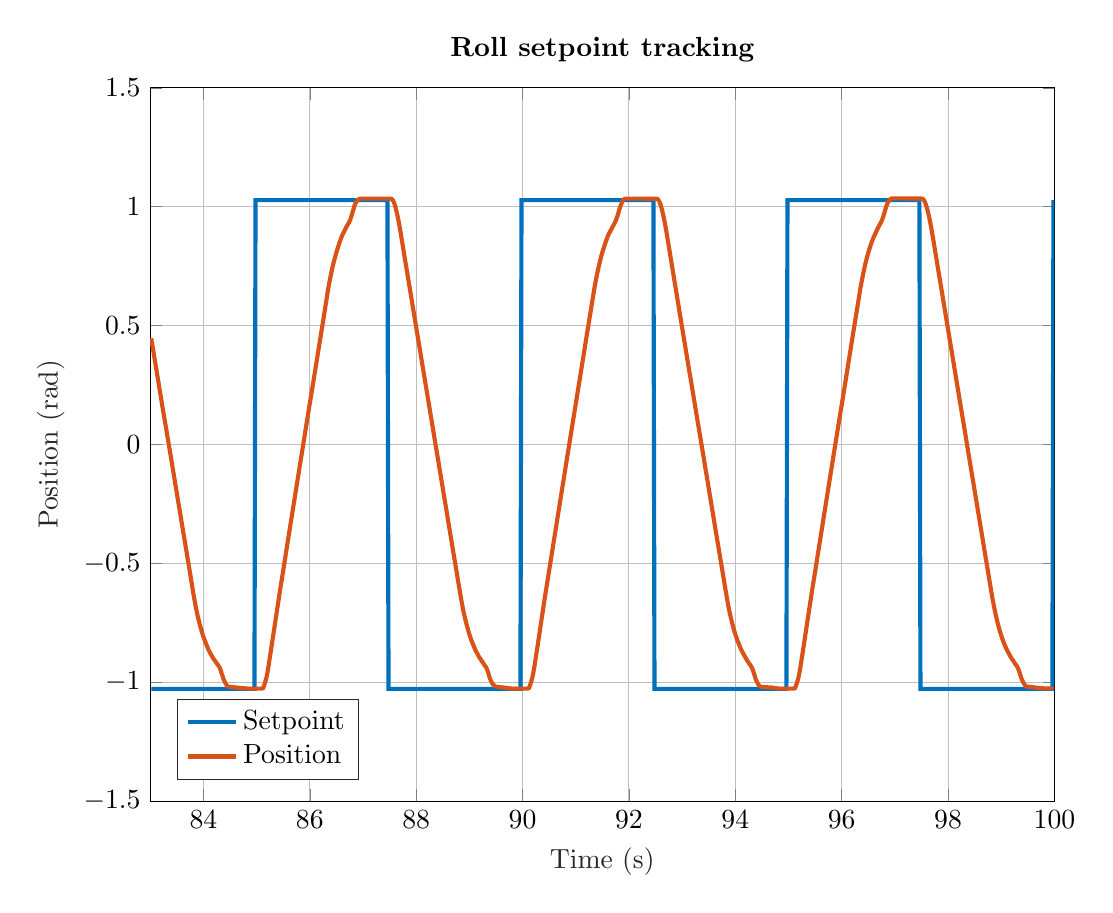
\begin{tikzpicture}

\begin{axis}[%
width=4.521in,
height=3.566in,
at={(0.758in,0.481in)},
scale only axis,
xmin=83,
xmax=100,
xlabel style={font=\color{white!15!black}},
xlabel={Time (s)},
ymin=-1.5,
ymax=1.5,
ylabel style={font=\color{white!15!black}},
ylabel={Position (rad)},
axis background/.style={fill=white},
title style={font=\bfseries},
title={Roll setpoint tracking},
xmajorgrids,
ymajorgrids,
legend style={at={(0.03,0.03)}, anchor=south west, legend cell align=left, align=left, draw=white!15!black}
]
\addplot [color=mycolor1, line width=1.5pt]
  table[row sep=crcr]{%
83.01917267	-1.02796056640625\\
84.95939636	-1.02796056640625\\
84.97940063	1.02796056640625\\
87.45979309	1.02796056640625\\
87.47977448	-1.02796056640625\\
89.96006775	-1.02796056640625\\
89.98009491	1.02796056640625\\
92.46042633	1.02796056640625\\
92.4803772	-1.02796056640625\\
94.96068573	-1.02796056640625\\
94.98072052	1.02796056640625\\
97.46098328	1.02796056640625\\
97.48095703	-1.02796056640625\\
99.96131897	-1.02796056640625\\
99.98136902	1.02796056640625\\
};
\addlegendentry{Setpoint}

\addplot [color=mycolor2, line width=1.5pt]
  table[row sep=crcr]{%
83.01917267	0.446307246093753\\
83.21920013	0.173258906249998\\
83.39933014	-0.0681409765625034\\
83.47921753	-0.176972753906256\\
83.65924835	-0.419987363281251\\
83.81925964	-0.637650957031255\\
83.85926819	-0.686738281250001\\
83.89938354	-0.7288823828125\\
83.93927765	-0.764083124999999\\
83.97928619	-0.795247148437497\\
84.01929474	-0.821244023437501\\
84.09941101	-0.865810195312505\\
84.17931366	-0.898104453125001\\
84.29943085	-0.935888789062503\\
84.31931305	-0.94638439453125\\
84.37934113	-0.987721132812496\\
84.39944458	-0.997732402343743\\
84.41933441	-1.0059673828125\\
84.43933105	-1.01274916015625\\
84.45934296	-1.0174318359375\\
84.47933197	-1.01936957031251\\
84.83938599	-1.02712015625001\\
85.0995636	-1.02679722656249\\
85.1194458	-1.02550548828125\\
85.13943481	-1.01565570312501\\
85.17941284	-0.985783515625002\\
85.19954681	-0.96495373046875\\
85.21952057	-0.938633867187505\\
85.31945801	-0.79250212890625\\
85.43946838	-0.614883496093753\\
85.49959564	-0.531079707031253\\
85.61950684	-0.360242910156245\\
85.71954346	-0.219762714843753\\
85.85955048	-0.0234133593749988\\
85.91955566	0.0602288671875044\\
85.97955322	0.144516992187505\\
86.0395813	0.225898613281245\\
86.27960205	0.56079046875\\
86.3396225	0.646370410156251\\
86.35961914	0.672044414062498\\
86.39974976	0.718063789062498\\
86.43963623	0.75810869140625\\
86.47962952	0.791856269531252\\
86.51963043	0.822051367187498\\
86.55963135	0.850954843750003\\
86.59978485	0.874368183593745\\
86.61964417	0.884702304687494\\
86.6796875	0.911506582031251\\
86.73968506	0.935242968750003\\
86.7596817	0.945254179687495\\
86.77967834	0.958333378906246\\
86.83972168	1.00402976562501\\
86.85972595	1.01484835937499\\
86.87970734	1.02227599609375\\
86.89983368	1.02744310546875\\
86.93975067	1.03390193359375\\
87.01973724	1.03422486328125\\
87.51979065	1.03390193359375\\
87.53978729	1.0329332421875\\
87.55978394	1.0279276171875\\
87.57977295	1.01936957031251\\
87.59990692	1.00725923828125\\
87.61981201	0.990789042968757\\
87.63980103	0.971412578124998\\
87.6598053	0.950098320312506\\
87.67980957	0.927007929687505\\
87.69992828	0.901818281250002\\
87.73979187	0.847079433593748\\
87.7798233	0.791694785156253\\
88.73993683	-0.509281113281247\\
88.81993866	-0.616498183593748\\
88.8399353	-0.643625390625004\\
88.87994385	-0.692066855468752\\
88.90008545	-0.713219628906245\\
88.93996429	-0.750196582031251\\
88.97995758	-0.783459746093754\\
89.00009155	-0.798638027343756\\
89.03997803	-0.824957910156243\\
89.0599823	-0.836422382812501\\
89.07997131	-0.84611068359375\\
89.10012054	-0.858221035156248\\
89.1199646	-0.867586406249998\\
89.15998077	-0.884217968749994\\
89.17998505	-0.893098828125005\\
89.31999969	-0.939441152343747\\
89.33998871	-0.950905664062503\\
89.36000061	-0.964146289062498\\
89.3800354	-0.979970566406251\\
89.40014648	-0.992080898437493\\
89.42004395	-1.0012848046875\\
89.44000244	-1.00790511718751\\
89.4600296	-1.0129107421875\\
89.48002625	-1.0163016796875\\
89.50016022	-1.018239296875\\
89.80017853	-1.02695869140625\\
90.10025024	-1.02679722656249\\
90.12010193	-1.02421361328125\\
90.14012146	-1.01339513671876\\
90.16012573	-0.999508535156252\\
90.18012238	-0.984007265624996\\
90.20025635	-0.963339003906256\\
90.22013092	-0.937342070312496\\
90.28011322	-0.851439199218746\\
90.36013794	-0.731142929687493\\
90.42016602	-0.642010703124996\\
90.7401886	-0.192474023437498\\
90.84018707	-0.0521552929687488\\
91.14022827	0.365248535156255\\
91.22019958	0.477794179687507\\
91.36021423	0.669783730468751\\
91.40035248	0.716287519531249\\
91.44024658	0.756493945312499\\
91.48025513	0.792340605468752\\
91.50040436	0.808649238281248\\
91.54025269	0.8367453125\\
91.5802536	0.862419316406246\\
91.60038757	0.874529648437502\\
91.62030792	0.88502525390625\\
91.74028778	0.935404394531247\\
91.76028442	0.945577109374995\\
91.7802887	0.958333378906246\\
91.80041504	0.972865722656252\\
91.8203125	0.989174355468748\\
91.84026337	1.002415078125\\
91.86031342	1.0137180859375\\
91.88027954	1.02340638671875\\
91.90042877	1.02970376953125\\
91.92029572	1.0329332421875\\
91.94029999	1.03422486328125\\
92.52037811	1.03374046875\\
92.54039001	1.03228724609374\\
92.5603714	1.02663576171875\\
92.58043671	1.01775490234375\\
92.60050201	1.00467576171874\\
92.62042999	0.988528476562493\\
92.66038513	0.948967988281254\\
92.68039703	0.925877597656253\\
92.70055389	0.900365117187505\\
92.94046021	0.572577929687498\\
93.10058594	0.354914375000007\\
93.16043854	0.275308906250004\\
93.22048187	0.19376580078125\\
93.30059814	0.0849340039062554\\
93.34046936	0.0322942968749942\\
93.52050018	-0.211689121093755\\
93.60061646	-0.321005351562505\\
93.6404953	-0.374775351562505\\
93.74054718	-0.509765527343745\\
93.78050232	-0.563374023437504\\
93.82050323	-0.617628457031245\\
93.86055756	-0.669299394531251\\
93.88052368	-0.692712734374993\\
93.90073395	-0.714026972656256\\
93.94054413	-0.751488378906245\\
93.98055267	-0.784428554687494\\
94.0007019	-0.798960976562498\\
94.04055786	-0.824796445312501\\
94.10071564	-0.858543906250006\\
94.14057922	-0.876144335937497\\
94.20072174	-0.900203535156251\\
94.24060059	-0.915058945312495\\
94.28057861	-0.927653750000005\\
94.30073547	-0.934112636718751\\
94.32056427	-0.94267056640625\\
94.36061096	-0.969474843750007\\
94.38063049	-0.985137656250004\\
94.40074158	-0.996117597656252\\
94.42059326	-1.00499857421875\\
94.44059753	-1.01210328125001\\
94.46063995	-1.0167859765625\\
94.48060608	-1.01936957031251\\
94.56060791	-1.02082279296874\\
94.70081329	-1.02276052734375\\
94.82070923	-1.02695869140625\\
95.10081482	-1.02679722656249\\
95.12071228	-1.02534400390626\\
95.14070892	-1.01549421875001\\
95.18074036	-0.986590859374999\\
95.20083618	-0.966083964843747\\
95.22074127	-0.941217343749997\\
95.28071594	-0.854507207031247\\
95.38075256	-0.705953398437501\\
95.44073486	-0.618274374999999\\
95.50090027	-0.533986249999998\\
95.70088196	-0.251249648437494\\
95.74074554	-0.195219042968745\\
95.84078979	-0.0550617773437523\\
95.96077728	0.112868574218751\\
96.00091553	0.166800058593751\\
96.06082153	0.250765234374995\\
96.10096741	0.306634375000002\\
96.22080994	0.475533535156245\\
96.30098724	0.585495664062506\\
96.34082794	0.641687714843755\\
96.36083984	0.668491992187498\\
96.40099335	0.714511386718755\\
96.44083405	0.756171074218756\\
96.46088409	0.774740234375003\\
96.50099182	0.807680429687494\\
96.5408783	0.836099433593745\\
96.56088257	0.849340117187495\\
96.60098267	0.871623105468757\\
96.68087006	0.910537773437497\\
96.74092865	0.935242968750003\\
96.76088715	0.945415644531252\\
96.78092957	0.958333378906246\\
96.84091187	1.00322242187499\\
96.86090088	1.0145254296875\\
96.88088989	1.02276052734375\\
96.90106201	1.02873484375\\
96.92089844	1.03309470703125\\
96.94093323	1.0351937890625\\
97.50112152	1.03470939453125\\
97.52097321	1.0334175390625\\
97.54103851	1.0290577734375\\
97.56098175	1.0217916015625\\
97.58106232	1.01048859375\\
97.60108948	0.995956132812495\\
97.62100983	0.979001640625\\
97.64096069	0.959948105468754\\
97.66101074	0.938310820312495\\
97.68099213	0.915058945312495\\
97.72100067	0.862742246093745\\
97.80110168	0.753587519531251\\
97.88104248	0.645563066406254\\
97.94104004	0.5640199609375\\
98.20117188	0.210235898437503\\
98.24107361	0.156627363281245\\
98.32102966	0.0486029296875046\\
98.36109924	-0.00613591796874857\\
98.44108582	-0.115936542968754\\
98.52109528	-0.223153613281255\\
98.56111145	-0.277730976562495\\
98.62114716	-0.359435566406248\\
98.72109222	-0.494425703125003\\
98.78115845	-0.576130292968756\\
98.82119751	-0.630384726562497\\
98.86117554	-0.678987656250001\\
98.90132904	-0.722262011718755\\
98.94119263	-0.758754550781248\\
98.98121643	-0.790402988281244\\
99.02119446	-0.818176074218755\\
99.061203	-0.841266542968754\\
99.10132599	-0.862257734375007\\
99.18123627	-0.895520957031252\\
99.30134583	-0.935081503906247\\
99.32120514	-0.944931171874998\\
99.34127045	-0.957364511718751\\
99.38127136	-0.985622050781245\\
99.42127991	-1.00435269531251\\
99.44121552	-1.01113458984375\\
99.46130371	-1.01581716796875\\
99.48130035	-1.01840076171875\\
99.54132843	-1.01969251953125\\
99.60134125	-1.0209842578125\\
99.66130066	-1.02340638671875\\
99.82130432	-1.02615134765625\\
99.98136902	-1.02615134765625\\
};
\addlegendentry{Position}

\end{axis}
\end{tikzpicture}%
		}
		\caption{Roll delay is 1.7 s}
	\end{subfigure}
	\begin{subfigure}[b]{0.5\textwidth}
		\centering
		\resizebox{\linewidth}{!}{
			% This file was created by matlab2tikz.
%
%The latest updates can be retrieved from
%  http://www.mathworks.com/matlabcentral/fileexchange/22022-matlab2tikz-matlab2tikz
%where you can also make suggestions and rate matlab2tikz.
%
\definecolor{mycolor1}{rgb}{0.00000,0.44700,0.74100}%
\definecolor{mycolor2}{rgb}{0.85000,0.32500,0.09800}%
%
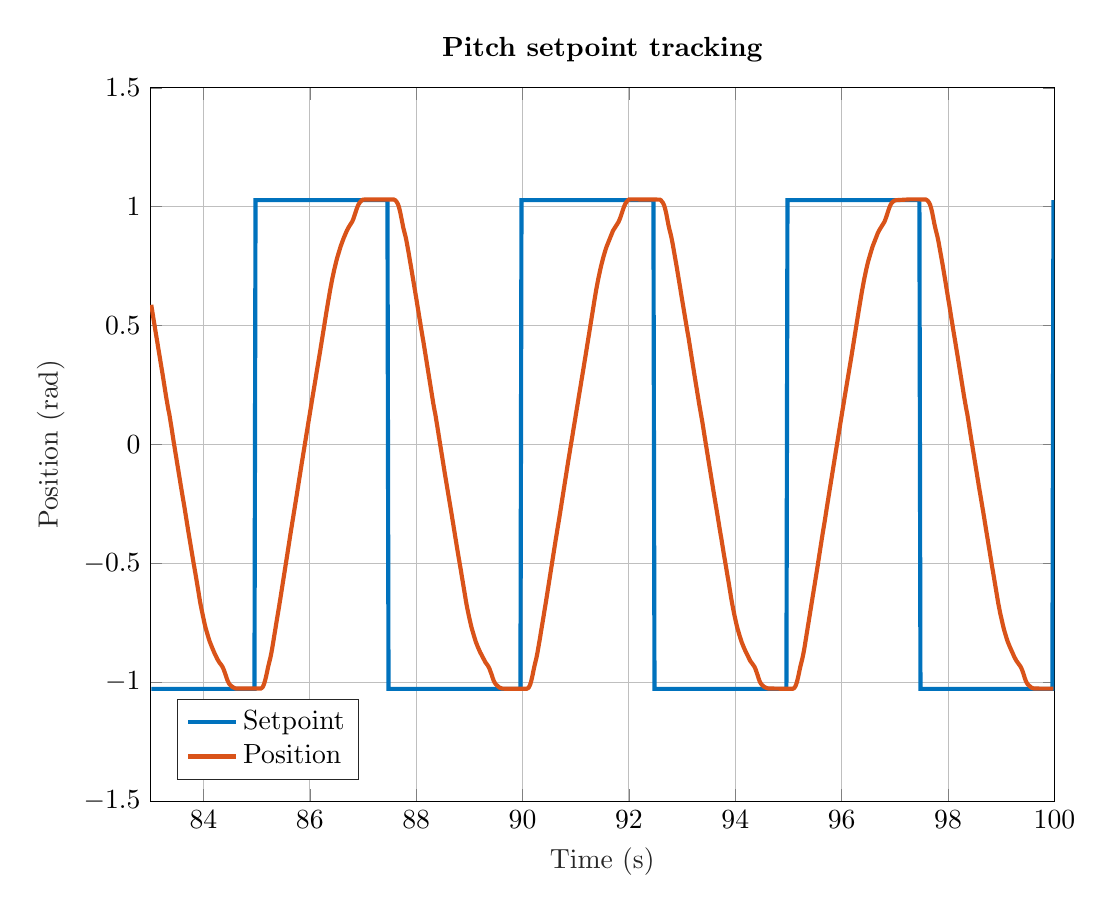
\begin{tikzpicture}

\begin{axis}[%
width=4.521in,
height=3.566in,
at={(0.758in,0.481in)},
scale only axis,
xmin=83,
xmax=100,
xlabel style={font=\color{white!15!black}},
xlabel={Time (s)},
ymin=-1.5,
ymax=1.5,
ylabel style={font=\color{white!15!black}},
ylabel={Position (rad)},
axis background/.style={fill=white},
title style={font=\bfseries},
title={Pitch setpoint tracking},
xmajorgrids,
ymajorgrids,
legend style={at={(0.03,0.03)}, anchor=south west, legend cell align=left, align=left, draw=white!15!black}
]
\addplot [color=mycolor1, line width=1.5pt]
  table[row sep=crcr]{%
83.01917267	-1.02796056640625\\
84.95939636	-1.02796056640625\\
84.97940063	1.02796056640625\\
87.45979309	1.02796056640625\\
87.47977448	-1.02796056640625\\
89.96006775	-1.02796056640625\\
89.98009491	1.02796056640625\\
92.46042633	1.02796056640625\\
92.4803772	-1.02796056640625\\
94.96068573	-1.02796056640625\\
94.98072052	1.02796056640625\\
97.46098328	1.02796056640625\\
97.48095703	-1.02796056640625\\
99.96131897	-1.02796056640625\\
99.98136902	1.02796056640625\\
};
\addlegendentry{Setpoint}

\addplot [color=mycolor2, line width=1.5pt]
  table[row sep=crcr]{%
83.01917267	0.587433339843756\\
83.05918121	0.530918300781252\\
83.17919159	0.367186171875005\\
83.23920441	0.285320136718752\\
83.29936981	0.199740234375\\
83.33920288	0.148553789062504\\
83.35921478	0.127078085937498\\
83.39933014	0.0716933593750042\\
83.43921661	0.0134021289062503\\
83.59934998	-0.206522070312502\\
83.63925171	-0.258354374999996\\
83.71925354	-0.370415625000007\\
83.81925964	-0.504114023437495\\
83.85926819	-0.555623437500003\\
83.93927765	-0.664293769531255\\
83.95927429	-0.687707089843755\\
84.01929474	-0.751326914062503\\
84.03928375	-0.770219082031247\\
84.07928467	-0.800898652343747\\
84.09941101	-0.816076933593749\\
84.11930084	-0.829479140624997\\
84.15929413	-0.852085058593744\\
84.19941711	-0.873560781250006\\
84.25931549	-0.901818281250002\\
84.29943085	-0.9169966796875\\
84.33931732	-0.928461152343743\\
84.35932922	-0.935727324218746\\
84.37934113	-0.945254179687495\\
84.41933441	-0.970443710937502\\
84.43933105	-0.984330195312495\\
84.45934296	-0.996279179687505\\
84.47933197	-1.00499857421875\\
84.49945068	-1.01081154296875\\
84.53935242	-1.01904664062501\\
84.59946442	-1.02615134765625\\
84.65936279	-1.02679722656249\\
85.07942963	-1.02647429687499\\
85.0995636	-1.0237293359375\\
85.1194458	-1.01856224609375\\
85.13943481	-1.00790511718751\\
85.15944672	-0.993049707031247\\
85.17941284	-0.974803457031257\\
85.21952057	-0.932659375\\
85.25944519	-0.89648970703125\\
85.27944183	-0.874368183593745\\
85.29961395	-0.849017109374998\\
85.33947754	-0.793793886718746\\
85.43946838	-0.657996328124995\\
85.57949829	-0.458740546875006\\
85.63952637	-0.371868867187501\\
85.7395401	-0.233487792968745\\
85.83953094	-0.0918772851562437\\
85.89969635	-0.00871945312499633\\
86.0395813	0.183270156250003\\
86.19974518	0.400126367187497\\
86.31960297	0.567410839843745\\
86.37963104	0.646208945312495\\
86.41962433	0.693843007812504\\
86.45962524	0.735341171875007\\
86.49979401	0.772479628906254\\
86.51963043	0.78878826171875\\
86.57962799	0.833192949218756\\
86.63964844	0.869685488281249\\
86.69981384	0.900849531250003\\
86.73968506	0.917158144531257\\
86.79982758	0.938310820312495\\
86.81971741	0.949290937499995\\
86.87970734	0.9898203515625\\
86.89983368	1.00176921875\\
86.91971588	1.0109730078125\\
86.93975067	1.0179163671875\\
86.95972443	1.023244921875\\
86.97973633	1.02728162109375\\
86.99984741	1.02970376953125\\
87.03973389	1.03067257812501\\
87.57977295	1.03034962890625\\
87.59990692	1.028250546875\\
87.61981201	1.0243751953125\\
87.63980103	1.0179163671875\\
87.6598053	1.00968126953126\\
87.67980957	0.995633183593753\\
87.69992828	0.97690255859375\\
87.75980377	0.909730390625001\\
87.79993439	0.874691113281244\\
87.81982422	0.853538339843752\\
87.85980988	0.80412806640625\\
87.97985077	0.644432734375002\\
88.09997559	0.479408886718744\\
88.13987732	0.426607695312498\\
88.23986816	0.286773398437504\\
88.31985474	0.174873632812506\\
88.3398819	0.1496840625\\
88.35987854	0.127239550781255\\
88.40000916	0.0721777539062458\\
88.43989563	0.0159856835937546\\
88.50001526	-0.0679795117187467\\
88.5398941	-0.123687167968754\\
88.60003662	-0.204907324218752\\
88.659935	-0.284674257812497\\
88.779953	-0.450666933593752\\
88.8399353	-0.528980625000003\\
88.90008545	-0.610846679687498\\
88.93996429	-0.664455234374998\\
88.95994568	-0.688353027343751\\
89.00009155	-0.730981464843751\\
89.03997803	-0.769250214843751\\
89.07997131	-0.800252714843751\\
89.1199646	-0.829479140624997\\
89.15998077	-0.852246542968757\\
89.2000885	-0.872753437499995\\
89.30014801	-0.915704882812506\\
89.33998871	-0.927815214843747\\
89.36000061	-0.934919921874993\\
89.3800354	-0.944608242187499\\
89.42004395	-0.968828964843752\\
89.44000244	-0.983200039062496\\
89.4600296	-0.994825976562495\\
89.48002625	-1.00322242187499\\
89.50016022	-1.00951978515624\\
89.56002045	-1.0217916015625\\
89.62004089	-1.02712015625001\\
89.84004974	-1.02776615234374\\
90.08008575	-1.02728162109375\\
90.10025024	-1.02534400390626\\
90.12010193	-1.0209842578125\\
90.14012146	-1.01178046875\\
90.16012573	-0.997732402343743\\
90.18012238	-0.978678808593756\\
90.22013092	-0.935404394531247\\
90.26010132	-0.898265917968743\\
90.28011322	-0.875821445312496\\
90.32011414	-0.824312031250003\\
90.44013977	-0.661225820312495\\
90.62017822	-0.405131992187506\\
90.70030212	-0.295654316406257\\
90.7401886	-0.238493398437498\\
90.80029297	-0.153074980468745\\
90.86021423	-0.0681409765625034\\
91.18025208	0.367993554687502\\
91.36021423	0.618274374999999\\
91.38025665	0.645240078124999\\
91.42025757	0.69287419921875\\
91.46028137	0.734533828124995\\
91.48025513	0.754071855468752\\
91.52025604	0.788949726562507\\
91.56024933	0.818983476562494\\
91.5802536	0.832385566406245\\
91.70042419	0.899234785156253\\
91.80041504	0.934435527343751\\
91.8203125	0.944123828125001\\
91.84026337	0.955426894531243\\
91.90042877	0.995794667968752\\
91.92029572	1.00645189453125\\
91.94029999	1.01549421875001\\
91.96030426	1.02227599609375\\
91.98033905	1.02728162109375\\
92.00043488	1.03034962890625\\
92.04031372	1.03099550781251\\
92.58043671	1.03002669921875\\
92.60050201	1.02744310546875\\
92.64041138	1.01614021484374\\
92.66038513	1.00693630859375\\
92.68039703	0.99191943359375\\
92.70055389	0.972704257812495\\
92.74043274	0.926039003906254\\
92.76040649	0.905693691406256\\
92.78044128	0.888577597656251\\
92.80053711	0.868878085937496\\
92.82043457	0.84611068359375\\
92.90057373	0.743899199218745\\
93.00054932	0.608101660156251\\
93.10058594	0.47408029296875\\
93.12045288	0.449213691406257\\
93.16043854	0.392698691406252\\
93.20056915	0.335537773437494\\
93.32048035	0.170352441406251\\
93.38049316	0.0939764062499933\\
93.42051697	0.0371384375000048\\
93.56048584	-0.156627363281245\\
93.66052246	-0.291617500000001\\
93.70068359	-0.347325195312493\\
93.74054718	-0.400449316406252\\
93.78050232	-0.455511093750005\\
93.82050323	-0.508635195312493\\
93.88052368	-0.588079160156255\\
93.92054749	-0.643625390625004\\
93.94054413	-0.669460859374993\\
93.98055267	-0.714995781249996\\
94.02059174	-0.755686601562502\\
94.04055786	-0.773448496093749\\
94.08055878	-0.804289531250006\\
94.12056732	-0.832062617187503\\
94.16056824	-0.854345742187505\\
94.20072174	-0.874206718750003\\
94.28057861	-0.910214785156256\\
94.32056427	-0.922325234374995\\
94.36061096	-0.935242968750003\\
94.38063049	-0.945415644531252\\
94.42059326	-0.971089589843757\\
94.44059753	-0.985622050781245\\
94.46063995	-0.997570917968744\\
94.48060608	-1.00548296875\\
94.50074768	-1.01145751953125\\
94.54064178	-1.01904664062501\\
94.58063507	-1.02389080078125\\
94.62065125	-1.0263128125\\
94.94071198	-1.02776615234374\\
95.08069611	-1.02744310546875\\
95.10081482	-1.02550548828125\\
95.12071228	-1.020661328125\\
95.14070892	-1.01129605468751\\
95.16072083	-0.997409453125002\\
95.18074036	-0.978840156250001\\
95.22074127	-0.936373203125001\\
95.26074219	-0.900203535156251\\
95.28071594	-0.879050878906256\\
95.30088043	-0.854022792968749\\
95.54079437	-0.520745585937505\\
95.60089111	-0.433550937500002\\
95.64076233	-0.376874492187497\\
95.68074036	-0.323104472656254\\
95.7207489	-0.265297675781255\\
95.76077271	-0.208944121093751\\
95.80088043	-0.153559394531257\\
95.98082733	0.0967214257812543\\
96.06082153	0.206037617187505\\
96.14084625	0.313900585937503\\
96.18087769	0.367186171875005\\
96.32080078	0.563535546875002\\
96.38080597	0.643948320312504\\
96.42087555	0.692551249999994\\
96.46088409	0.735018222656251\\
96.48086548	0.754717792968748\\
96.50099182	0.772641152343752\\
96.5408783	0.803159199218754\\
96.5809021	0.8327085546875\\
96.68087006	0.890192343750002\\
96.70102692	0.899234785156253\\
96.76088715	0.921194902343757\\
96.80101776	0.935404394531247\\
96.82090759	0.946222988281249\\
96.84091187	0.958817773437502\\
96.88088989	0.986590859374999\\
96.90106201	0.999185605468753\\
96.92089844	1.009035390625\\
96.94093323	1.01646314453124\\
96.98092651	1.02469814453126\\
97.02093506	1.02760457031251\\
97.30109406	1.03115697265625\\
97.58106232	1.03051111328125\\
97.60108948	1.02808908203124\\
97.62100983	1.02405214843751\\
97.64096069	1.01775490234375\\
97.66101074	1.00887392578124\\
97.68099213	0.994664492187496\\
97.70115662	0.975933691406254\\
97.74104309	0.929914296874998\\
97.76100922	0.909568925781244\\
97.80110168	0.87339931640625\\
97.82102966	0.851762128906245\\
97.90119934	0.751488378906245\\
97.94104004	0.698202753906244\\
97.98104095	0.64297951171875\\
98.00115967	0.614883496093753\\
98.02106476	0.589209492187507\\
98.06108093	0.532371523437504\\
98.1810379	0.369123847656255\\
98.22109985	0.313254707031248\\
98.26107788	0.257708515624998\\
98.30119324	0.201677910156249\\
98.34111786	0.150491445312497\\
98.36109924	0.128369843749994\\
98.38111877	0.100758222656253\\
98.42110443	0.0427899414062551\\
98.58111572	-0.178103066406251\\
98.66114807	-0.284028359375\\
98.72109222	-0.367347675781247\\
98.76113892	-0.421602070312503\\
98.82119751	-0.504598437499993\\
98.86117554	-0.557399589843754\\
98.92116547	-0.638135351562497\\
98.94119263	-0.665101054687497\\
98.98121643	-0.710959023437496\\
99.04116821	-0.769250214843751\\
99.061203	-0.785881835937502\\
99.10132599	-0.815915468750006\\
99.12120056	-0.829156074218744\\
99.16119385	-0.851277734375003\\
99.24119568	-0.891322675781254\\
99.28121948	-0.908761640625002\\
99.36122131	-0.933789707031252\\
99.38127136	-0.942832031250006\\
99.40136719	-0.954135097656248\\
99.42127991	-0.967052832031257\\
99.44121552	-0.981746699218746\\
99.46130371	-0.994179980468743\\
99.48130035	-1.00322242187499\\
99.50144196	-1.009842734375\\
99.56127167	-1.0217916015625\\
99.60134125	-1.02615134765625\\
99.70145416	-1.02679722656249\\
99.98136902	-1.02712015625001\\
};
\addlegendentry{Position}

\end{axis}
\end{tikzpicture}%
		}
		\caption{Pitch delay is 1.7 s}
	\end{subfigure}
	\caption{Tracking of setpoint jumps between limits}
	\label{square_excite}
\end{figure}

%\begin{figure}[h] \label{ fig7} \begin{minipage}[b]{0.50\linewidth}\centering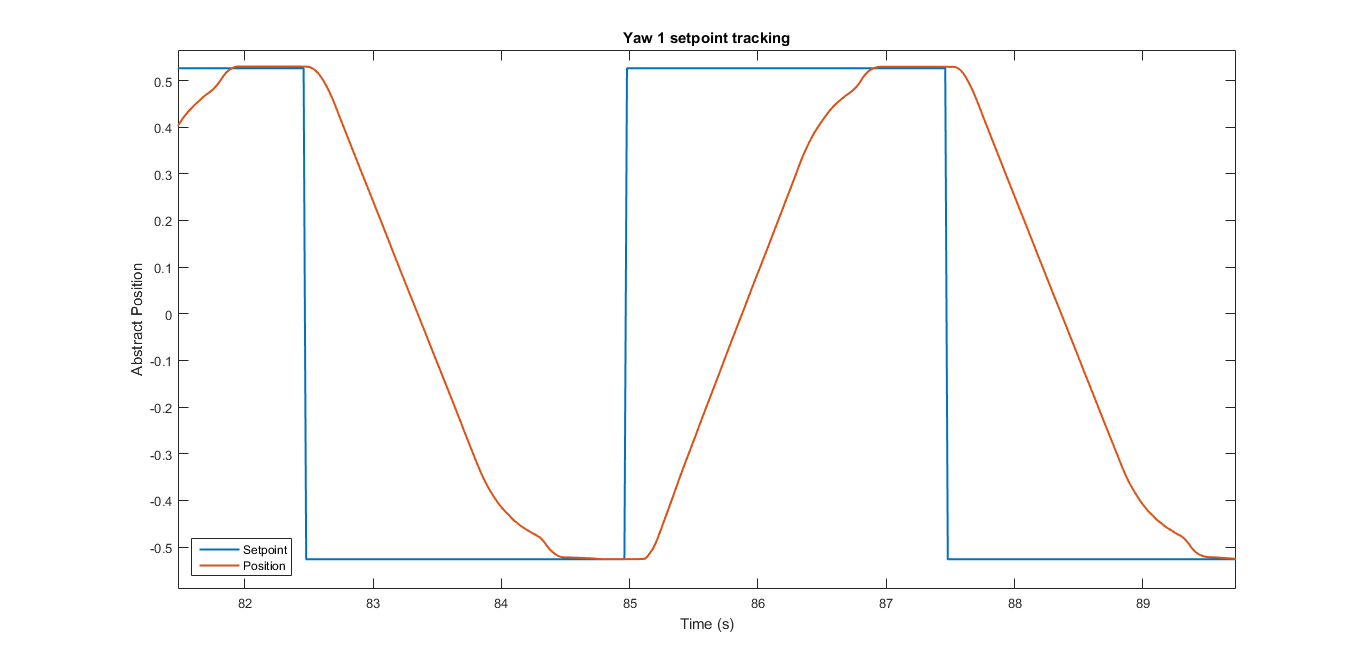
\includegraphics[width=0.70\linewidth]{extreme_yaw1.png} \caption{} \end{minipage} \begin{minipage}[b]{0.50\linewidth}\centering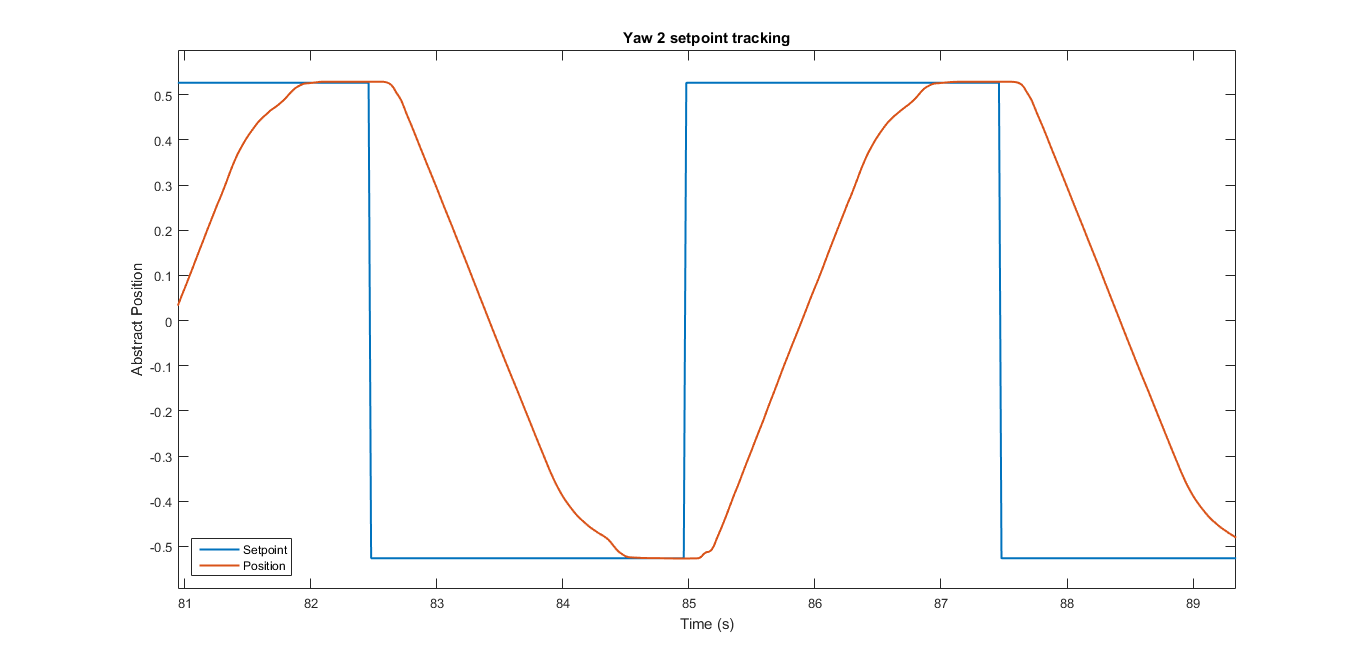
\includegraphics[width=0.70\linewidth]{extreme_yaw2.png} \caption{} \end{minipage} \begin{minipage}[b]{0.50\linewidth}\centering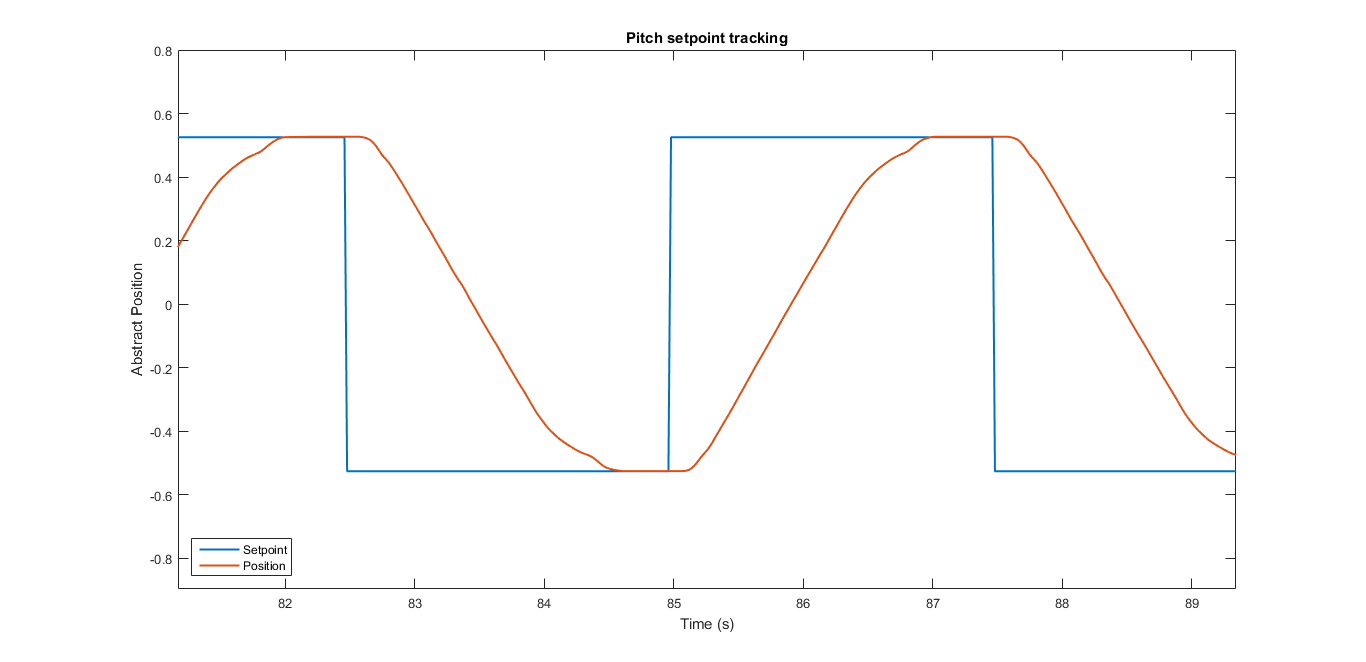
\includegraphics[width=0.70\linewidth]{extreme_pitch.png} \caption{} \end{minipage}\hfill \begin{minipage}[b]{0.50\linewidth}\centering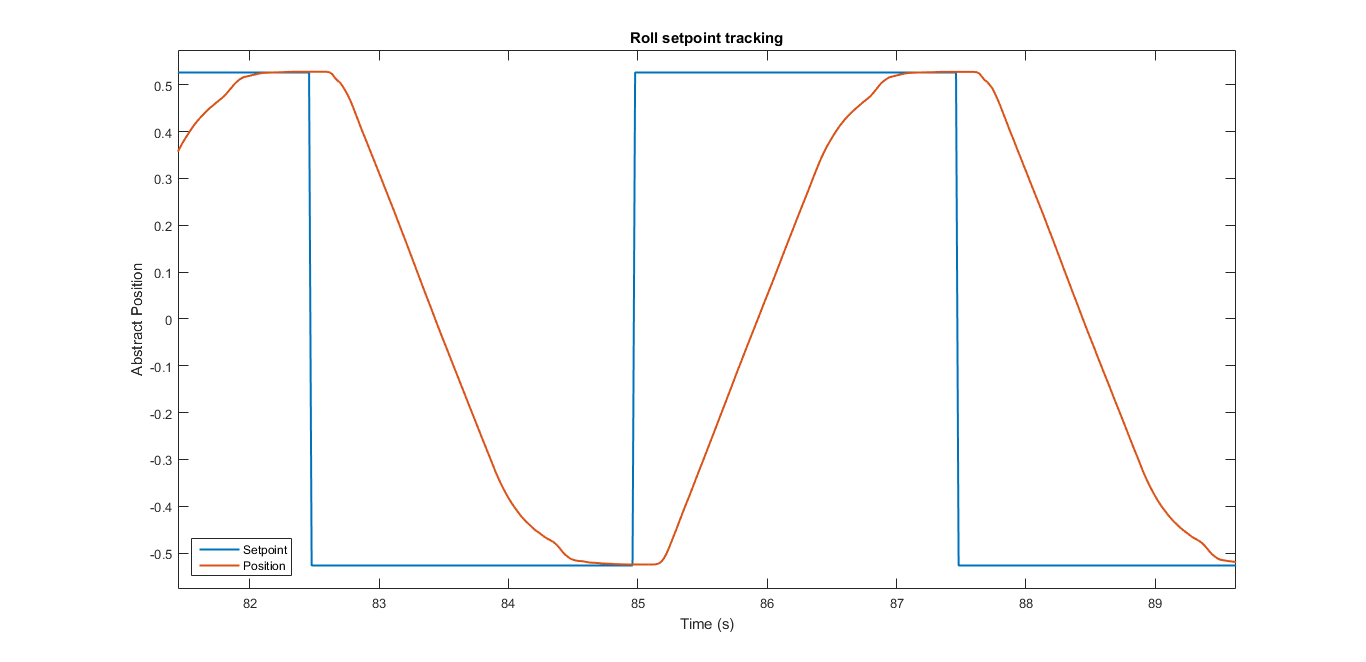
\includegraphics[width=0.70\linewidth]{extreme_roll.png} \caption{} \end{minipage} \end{figure}
%
%\begin{figure}[h] \label{ fig7} \begin{minipage}[b]{0.50\linewidth}\centering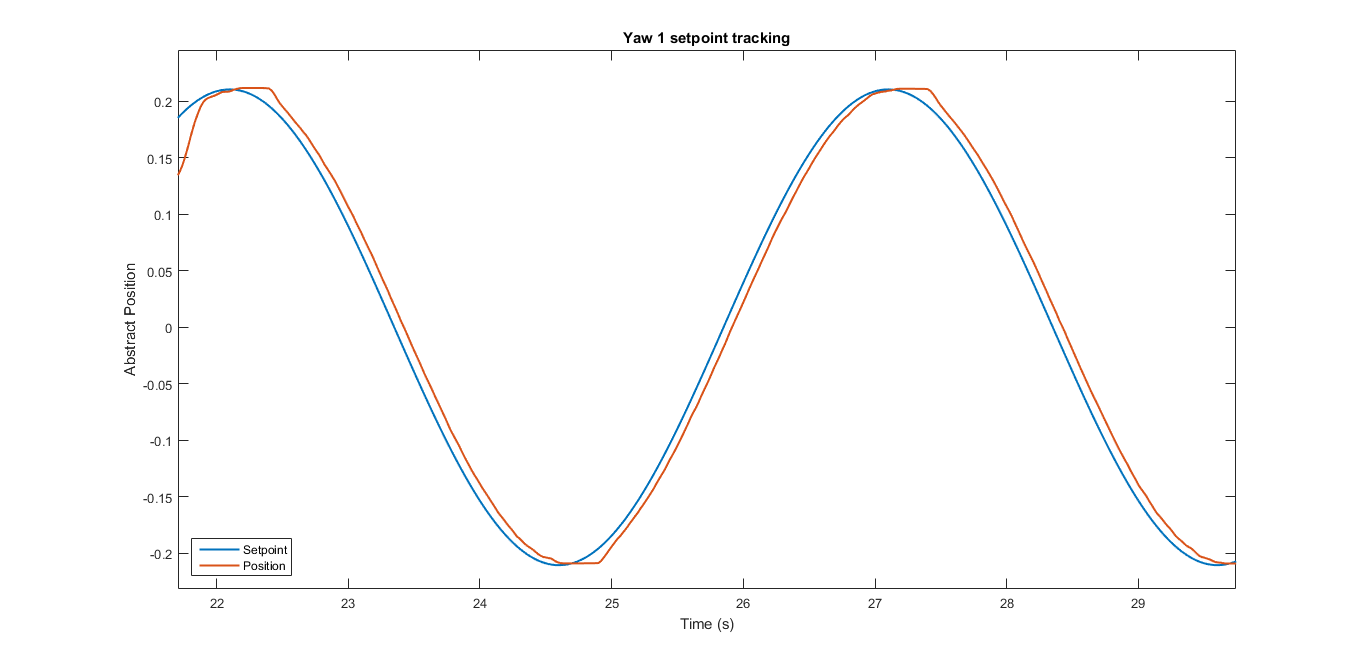
\includegraphics[width=0.70\linewidth]{mild_yaw1.png} \caption{The yaw setpoint tracking lag in this case is 50 ms} \end{minipage} \begin{minipage}[b]{0.50\linewidth}\centering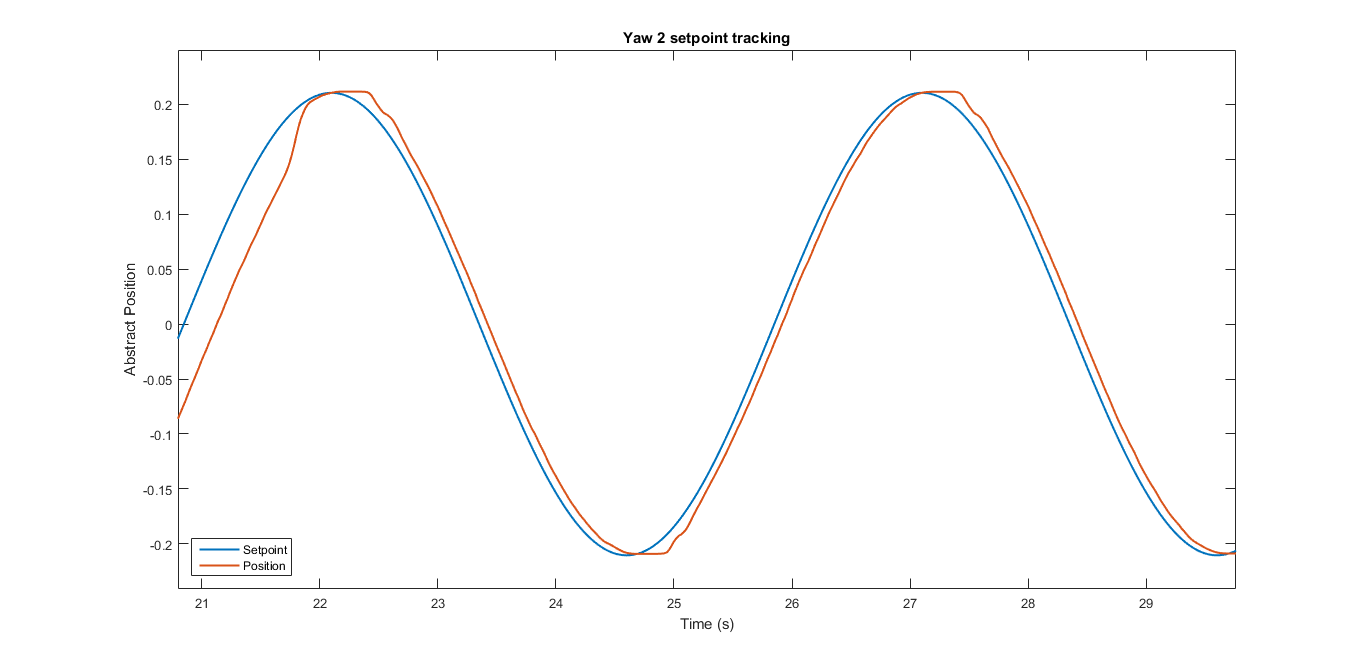
\includegraphics[width=0.70\linewidth]{mild_yaw2.png} \caption{} \end{minipage} \begin{minipage}[b]{0.50\linewidth}\centering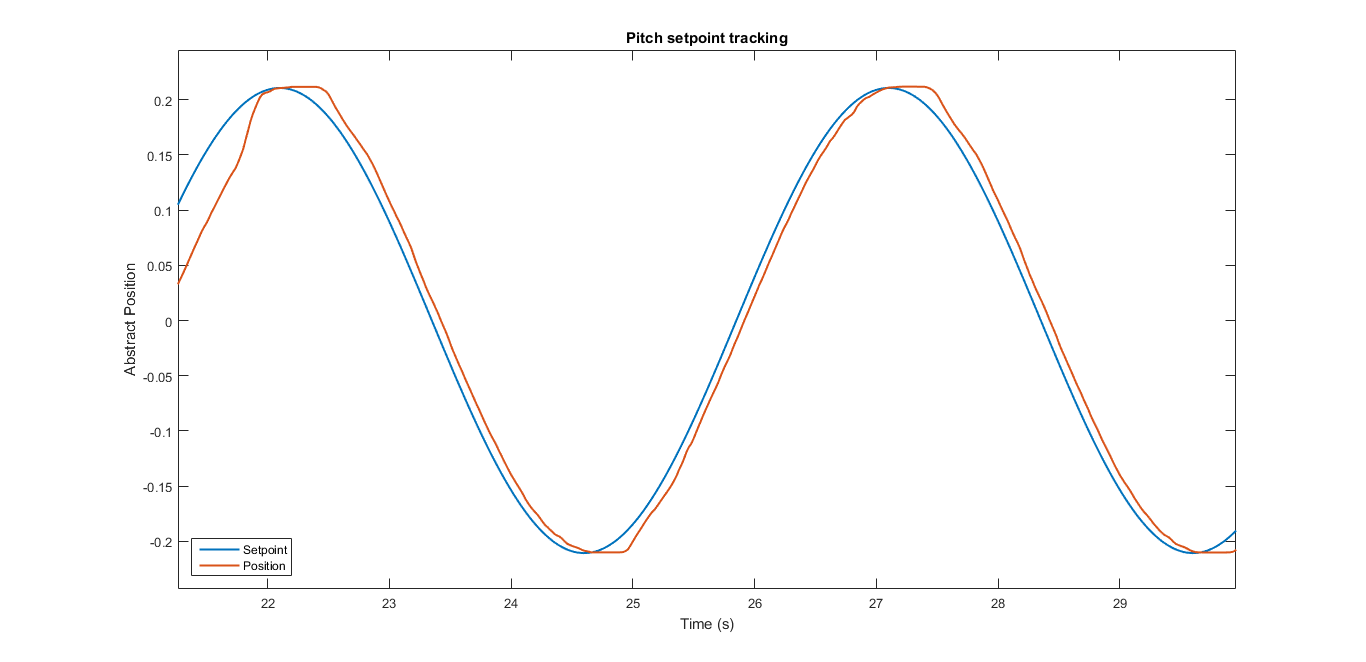
\includegraphics[width=0.70\linewidth]{mild_pitch.png} \caption{} \end{minipage}\hfill \begin{minipage}[b]{0.50\linewidth}\centering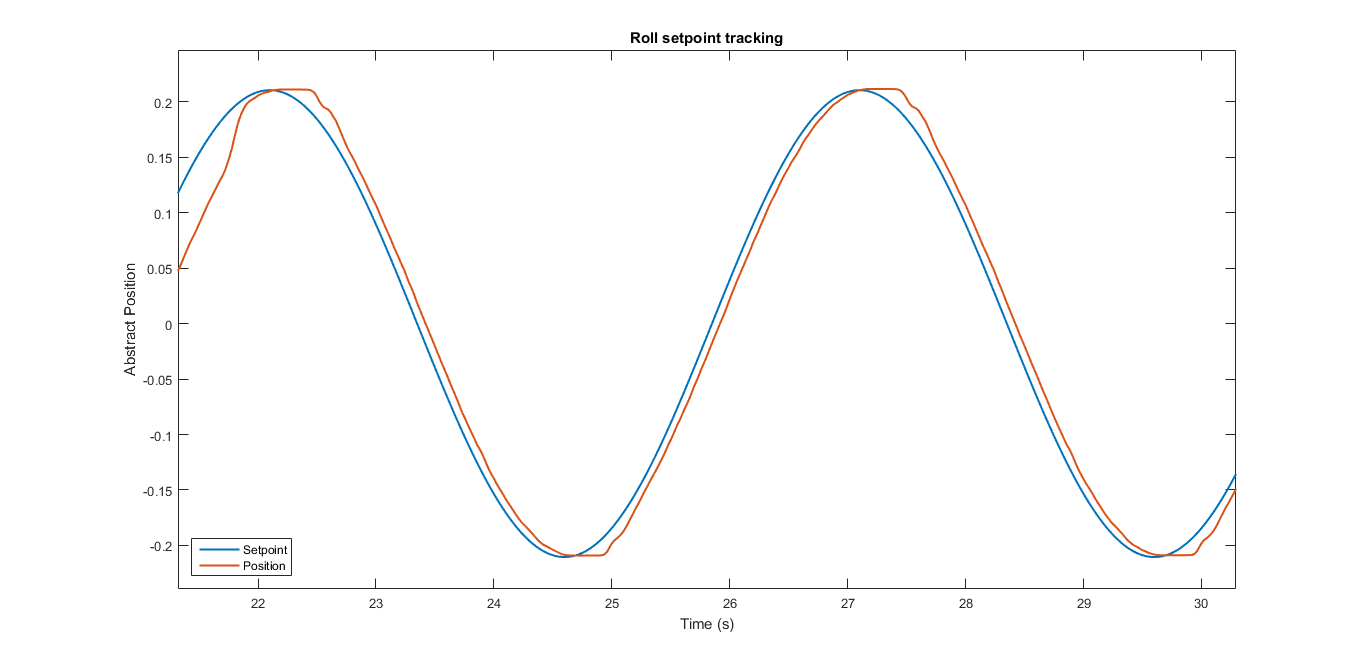
\includegraphics[width=0.70\linewidth]{mild_roll.png} \caption{} \end{minipage} \end{figure}


For the measurements with sinusoidal setpoint signals, see \figref{square_excite}. This is much more similar to normal operations, where instead of jumps, the operator makes continuous moves. The delay defined in these graphs is the time between the setpoints and positions being at the same value.

\begin{figure}
	\begin{subfigure}[b]{0.5\textwidth}
		\centering
		\resizebox{\linewidth}{!}{
			% This file was created by matlab2tikz.
%
%The latest updates can be retrieved from
%  http://www.mathworks.com/matlabcentral/fileexchange/22022-matlab2tikz-matlab2tikz
%where you can also make suggestions and rate matlab2tikz.
%
\definecolor{mycolor1}{rgb}{0.00000,0.44700,0.74100}%
\definecolor{mycolor2}{rgb}{0.85000,0.32500,0.09800}%
%
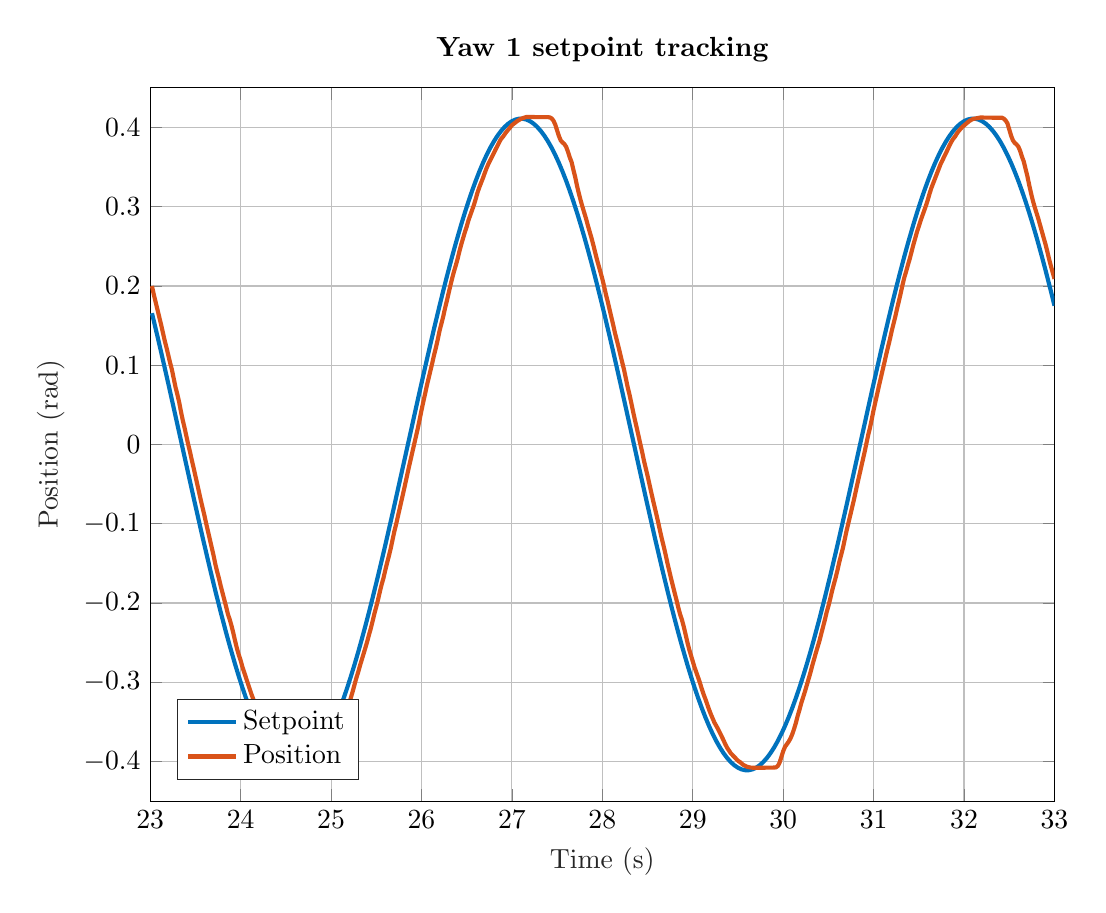
\begin{tikzpicture}

\begin{axis}[%
width=4.521in,
height=3.566in,
at={(0.758in,0.481in)},
scale only axis,
xmin=23,
xmax=33,
xlabel style={font=\color{white!15!black}},
xlabel={Time (s)},
ymin=-0.45,
ymax=0.45,
ylabel style={font=\color{white!15!black}},
ylabel={Position (rad)},
axis background/.style={fill=white},
title style={font=\bfseries},
title={Yaw 1 setpoint tracking},
xmajorgrids,
ymajorgrids,
legend style={at={(0.03,0.03)}, anchor=south west, legend cell align=left, align=left, draw=white!15!black}
]
\addplot [color=mycolor1, line width=1.5pt]
  table[row sep=crcr]{%
23.0191555	0.165668769531251\\
23.0791626	0.136850136718749\\
23.11917114	0.117195410156249\\
23.19929695	0.0770482421875016\\
23.3391819	0.00516695312499849\\
23.47919846	-0.0668738281249972\\
23.57920647	-0.117195410156249\\
23.65921402	-0.15615916015625\\
23.71923447	-0.1843680859375\\
23.77923203	-0.211529414062497\\
23.83923912	-0.237488769531247\\
23.87924385	-0.254054121093752\\
23.93925476	-0.277686171874997\\
23.9792614	-0.292572246093748\\
24.01925659	-0.306719218749997\\
24.05926514	-0.32009140625\\
24.09938622	-0.332655000000003\\
24.1392746	-0.344378320312501\\
24.17927551	-0.35523166015625\\
24.21928978	-0.36518767578125\\
24.25928879	-0.374221191406249\\
24.2994175	-0.382309394531248\\
24.33930206	-0.38943185546875\\
24.37930679	-0.395570585937499\\
24.41931152	-0.400710058593752\\
24.45931435	-0.404837304687497\\
24.49943924	-0.407941894531248\\
24.53932953	-0.410015976562498\\
24.57933235	-0.41105435546875\\
24.61933899	-0.41105435546875\\
24.65933609	-0.410015976562498\\
24.69947052	-0.407941894531248\\
24.73935127	-0.404837304687497\\
24.77935219	-0.400710058593752\\
24.81936455	-0.395570585937499\\
24.85939026	-0.38943185546875\\
24.89950562	-0.382309394531248\\
24.93938637	-0.374221191406249\\
24.97940445	-0.36518767578125\\
25.01939392	-0.35523166015625\\
25.05941391	-0.344378320312501\\
25.09952736	-0.332655000000003\\
25.13941765	-0.32009140625\\
25.17942429	-0.306719218749997\\
25.21941948	-0.292572246093748\\
25.2595253	-0.277686171874997\\
25.29954147	-0.262098671875002\\
25.33945274	-0.245849082031249\\
25.37944412	-0.228978476562503\\
25.41944885	-0.211529414062497\\
25.45945358	-0.193546015625003\\
25.51947403	-0.165668769531251\\
25.57947159	-0.136850136718749\\
25.61948204	-0.117195410156249\\
25.69965935	-0.0770482421875016\\
25.89969635	0.0258184765624989\\
25.95955086	0.0566571875000008\\
26.03957939	0.0972446484375027\\
26.09970474	0.127062910156248\\
26.13957214	0.146550937500002\\
26.17958832	0.165668769531251\\
26.23957825	0.193546015625003\\
26.27958679	0.211529414062497\\
26.33958435	0.237488769531247\\
26.37959862	0.254054121093752\\
26.43959999	0.277686171874997\\
26.47961998	0.292572246093748\\
26.51965904	0.306719218749997\\
26.559618	0.32009140625\\
26.59978867	0.332655000000003\\
26.63961983	0.344378320312501\\
26.67969131	0.35523166015625\\
26.71968079	0.36518767578125\\
26.7596817	0.374221191406249\\
26.79981041	0.382309394531248\\
26.83969688	0.38943185546875\\
26.8796978	0.395570585937499\\
26.91968918	0.400710058593752\\
26.95970345	0.404837304687497\\
26.9998188	0.407941894531248\\
27.03972244	0.410015976562498\\
27.07970428	0.41105435546875\\
27.11972046	0.41105435546875\\
27.15972137	0.410015976562498\\
27.19987488	0.407941894531248\\
27.23973846	0.404837304687497\\
27.27972794	0.400710058593752\\
27.31974983	0.395570585937499\\
27.3597641	0.38943185546875\\
27.39987946	0.382309394531248\\
27.43976212	0.374221191406249\\
27.47976685	0.36518767578125\\
27.51978683	0.35523166015625\\
27.55976677	0.344378320312501\\
27.59990501	0.332655000000003\\
27.63977814	0.32009140625\\
27.67980003	0.306719218749997\\
27.71977997	0.292572246093748\\
27.75979042	0.277686171874997\\
27.79992867	0.262098671875002\\
27.83981323	0.245849082031249\\
27.87981415	0.228978476562503\\
27.91983032	0.211529414062497\\
27.97982025	0.1843680859375\\
28.01981544	0.165668769531251\\
28.07985115	0.136850136718749\\
28.11987686	0.117195410156249\\
28.19997215	0.0770482421875016\\
28.31985855	0.0154976171874992\\
28.47991753	-0.0668738281249972\\
28.57987976	-0.117195410156249\\
28.65989304	-0.15615916015625\\
28.71993256	-0.1843680859375\\
28.75995255	-0.202601699218746\\
28.80004501	-0.220323515624997\\
28.8399334	-0.237488769531247\\
28.87992287	-0.254054121093752\\
28.93993759	-0.277686171874997\\
28.97994614	-0.292572246093748\\
29.01994705	-0.306719218749997\\
29.05997849	-0.32009140625\\
29.10009575	-0.332655000000003\\
29.13996696	-0.344378320312501\\
29.17998505	-0.35523166015625\\
29.21994209	-0.36518767578125\\
29.25997353	-0.374221191406249\\
29.30012321	-0.382309394531248\\
29.34000587	-0.38943185546875\\
29.3800087	-0.395570585937499\\
29.41999435	-0.400710058593752\\
29.46001816	-0.404837304687497\\
29.50014114	-0.407941894531248\\
29.54003143	-0.410015976562498\\
29.58001518	-0.41105435546875\\
29.62005615	-0.41105435546875\\
29.66002274	-0.410015976562498\\
29.70015717	-0.407941894531248\\
29.74006462	-0.404837304687497\\
29.78003311	-0.400710058593752\\
29.82004356	-0.395570585937499\\
29.86007118	-0.38943185546875\\
29.90019608	-0.382309394531248\\
29.94006538	-0.374221191406249\\
29.98004532	-0.36518767578125\\
30.02007484	-0.35523166015625\\
30.06008911	-0.344378320312501\\
30.10021591	-0.332655000000003\\
30.14009857	-0.32009140625\\
30.18009949	-0.306719218749997\\
30.22017097	-0.292572246093748\\
30.26011658	-0.277686171874997\\
30.30026627	-0.262098671875002\\
30.34012604	-0.245849082031249\\
30.40029907	-0.220323515624997\\
30.4601326	-0.193546015625003\\
30.52017593	-0.165668769531251\\
30.58013344	-0.136850136718749\\
30.62013245	-0.117195410156249\\
30.70029259	-0.0770482421875016\\
30.84021378	-0.00516695312499849\\
30.980196	0.0668738281249972\\
31.08020401	0.117195410156249\\
31.1602459	0.15615916015625\\
31.22019577	0.1843680859375\\
31.28022957	0.211529414062497\\
31.34022331	0.237488769531247\\
31.38021278	0.254054121093752\\
31.44024277	0.277686171874997\\
31.48025322	0.292572246093748\\
31.520298	0.306719218749997\\
31.56042099	0.32009140625\\
31.60041428	0.332655000000003\\
31.64028549	0.344378320312501\\
31.68028259	0.35523166015625\\
31.72029877	0.36518767578125\\
31.76030731	0.374221191406249\\
31.80044556	0.382309394531248\\
31.84035492	0.38943185546875\\
31.88029289	0.395570585937499\\
31.92034912	0.400710058593752\\
31.96029282	0.404837304687497\\
32.00043488	0.407941894531248\\
32.04032898	0.410015976562498\\
32.08035278	0.41105435546875\\
32.12031555	0.41105435546875\\
32.16034317	0.410015976562498\\
32.20049286	0.407941894531248\\
32.24038315	0.404837304687497\\
32.28037262	0.400710058593752\\
32.32038116	0.395570585937499\\
32.36040878	0.38943185546875\\
32.40048218	0.382309394531248\\
32.44039536	0.374221191406249\\
32.48039627	0.36518767578125\\
32.5204277	0.35523166015625\\
32.56040192	0.344378320312501\\
32.60052109	0.332655000000003\\
32.64037704	0.32009140625\\
32.68041992	0.306719218749997\\
32.72045135	0.292572246093748\\
32.7604332	0.277686171874997\\
32.8005867	0.262098671875002\\
32.86040115	0.237488769531247\\
32.90053558	0.220323515624997\\
32.96042633	0.193546015625003\\
33.00058746	0.175073710937497\\
};
\addlegendentry{Setpoint}

\addplot [color=mycolor2, line width=1.5pt]
  table[row sep=crcr]{%
23.0191555	0.199901718749999\\
23.03915405	0.189406054687502\\
23.0992794	0.160987089843751\\
23.11917114	0.151783203124999\\
23.15916443	0.131437792968747\\
23.17917252	0.122556875000001\\
23.21917725	0.103341757812501\\
23.23917961	0.0946223046874977\\
23.27918243	0.0725007031250016\\
23.29930305	0.0634583007812495\\
23.31919098	0.0537700000000001\\
23.3391819	0.0418211132812516\\
23.35918236	0.0308410546874995\\
23.37919235	0.0213142382812492\\
23.41919327	0.000322949218748647\\
23.43920135	-0.00904240234375209\\
23.459198	-0.0195380468749988\\
23.47919846	-0.0292263476562482\\
23.55920982	-0.0702400976562529\\
23.59934044	-0.0896166796875022\\
23.6192131	-0.0999508593749994\\
23.67922783	-0.129661601562503\\
23.69934082	-0.139511386718752\\
23.71923447	-0.150652910156253\\
23.73923111	-0.160179726562497\\
23.75923157	-0.168737714843751\\
23.77923203	-0.17842599609375\\
23.83923912	-0.204745878906252\\
23.8592453	-0.214111210937503\\
23.87924385	-0.22089298828125\\
23.89936638	-0.228966582031248\\
23.91924667	-0.23817044921875\\
23.93925476	-0.248181699218748\\
23.95925522	-0.257547050781248\\
23.9792614	-0.265459160156247\\
23.99937439	-0.272402421875\\
24.01925659	-0.280637460937498\\
24.05926514	-0.294524003906247\\
24.11927795	-0.315192363281248\\
24.21928978	-0.345710468749999\\
24.23929024	-0.351039023437501\\
24.27929878	-0.359274062499999\\
24.37930679	-0.382525957031248\\
24.39942551	-0.386239824218748\\
24.41931152	-0.389469238281251\\
24.47932053	-0.395928124999998\\
24.51931763	-0.400449316406252\\
24.57933235	-0.406262285156252\\
24.59946823	-0.407392597656248\\
24.63933563	-0.408361425781251\\
24.69947052	-0.408522871093751\\
24.89950562	-0.408361425781251\\
24.9193821	-0.407876992187497\\
24.93938637	-0.406262285156252\\
24.9593811	-0.402064042968753\\
24.99950981	-0.387370117187501\\
25.01939392	-0.382364492187499\\
25.05941391	-0.375259746093747\\
25.07941818	-0.371061503906247\\
25.09952736	-0.365571464843747\\
25.11941338	-0.35878966796875\\
25.13941765	-0.35120052734375\\
25.15943146	-0.342803984375003\\
25.17942429	-0.335214843750002\\
25.19954681	-0.326656816406249\\
25.21941948	-0.319390644531254\\
25.23942566	-0.311478535156247\\
25.27942657	-0.294685488281253\\
25.29954147	-0.287419277343751\\
25.31944466	-0.279184199218747\\
25.37944412	-0.256578203125002\\
25.39957237	-0.248666132812502\\
25.41944885	-0.24010810546875\\
25.43946648	-0.232034531250001\\
25.45945358	-0.222992128906249\\
25.47947884	-0.213303847656249\\
25.49957657	-0.204907324218752\\
25.51947403	-0.195864941406249\\
25.53948212	-0.185853691406251\\
25.55951691	-0.17664982421875\\
25.57947159	-0.168576250000001\\
25.59960938	-0.158565000000003\\
25.61948204	-0.149361132812501\\
25.63947678	-0.140641679687498\\
25.65950775	-0.131276328124997\\
25.69965935	-0.109639140624999\\
25.71951675	-0.100596738281247\\
25.77954102	-0.0704015625000025\\
25.79967308	-0.0603903320312469\\
25.85951996	-0.0292263476562482\\
25.95955086	0.0205068750000024\\
25.97954559	0.0314869335937473\\
25.99969482	0.0429514257812471\\
26.01956367	0.0536085351562505\\
26.03957939	0.0637812499999981\\
26.05957413	0.0744383593750015\\
26.11956024	0.103018808593752\\
26.13957214	0.1131915234375\\
26.15955734	0.122233925781252\\
26.17958832	0.132406640625\\
26.19974518	0.143386699218752\\
26.23957825	0.1611485546875\\
26.25958061	0.171644199218747\\
26.27958679	0.180848066406249\\
26.31958199	0.200547597656247\\
26.33958435	0.209912949218747\\
26.35961342	0.218470937500001\\
26.37959862	0.226060097656251\\
26.39978218	0.234456621093749\\
26.41959763	0.243821972656249\\
26.43959999	0.252379941406247\\
26.47961998	0.267881210937503\\
26.49975395	0.274824511718748\\
26.51965904	0.282898046874998\\
26.57962227	0.302274628906247\\
26.59978867	0.309863828125003\\
26.61962128	0.317937382812502\\
26.63961983	0.324557714843749\\
26.67969131	0.336183632812499\\
26.69979858	0.342642519531253\\
26.71968079	0.348616953125003\\
26.73966599	0.353945507812497\\
26.81968689	0.37235328125\\
26.85968971	0.381395683593752\\
26.8796978	0.3855939453125\\
26.89981651	0.388177480468748\\
26.93969345	0.394636367187502\\
26.97970009	0.399964921874997\\
26.9998188	0.40287140625\\
27.05970955	0.408199960937502\\
27.09983826	0.41094494140625\\
27.1397171	0.4125596875\\
27.15972137	0.413205566406248\\
27.39987946	0.413044121093748\\
27.41974258	0.4127211328125\\
27.43976212	0.411429374999997\\
27.45976257	0.408522871093751\\
27.47976685	0.403517265624998\\
27.51978683	0.389146289062502\\
27.53976059	0.383656269531251\\
27.55976677	0.381072753906253\\
27.57977867	0.379135078125003\\
27.59990501	0.375582714843752\\
27.6197834	0.369446796875003\\
27.63977814	0.362180546875003\\
27.65979767	0.356367578125003\\
27.67980003	0.346679335937502\\
27.69993019	0.337475410156252\\
27.71977997	0.326495390624999\\
27.73979187	0.316968574218748\\
27.75979042	0.308087617187503\\
27.77978325	0.300014042968748\\
27.81982803	0.284997187499997\\
27.83981323	0.276439218749999\\
27.87981415	0.260615000000001\\
27.89992714	0.251895507812499\\
27.93980408	0.233649238281252\\
27.99995804	0.208944121093751\\
28.01981544	0.199417304687501\\
28.03981781	0.189244609375002\\
28.05982971	0.180202187500001\\
28.09995842	0.160502675781252\\
28.11987686	0.150975839843753\\
28.13983154	0.140641679687498\\
28.17984009	0.12271833984375\\
28.21988106	0.1035032421875\\
28.23985672	0.0944608203124986\\
28.27983856	0.0725007031250016\\
28.3000145	0.0631353515625008\\
28.31985855	0.052639707031247\\
28.33985138	0.041659648437502\\
28.35985947	0.0311640039062482\\
28.37986183	0.0213142382812492\\
28.41988564	0.000645878906247788\\
28.43987274	-0.00920386718750166\\
28.45988464	-0.0203454101562528\\
28.49998093	-0.0393990429687534\\
28.5398941	-0.0599059179687487\\
28.55990982	-0.0700786328125034\\
28.60004807	-0.0894552148437526\\
28.61990929	-0.0994664453125012\\
28.63990402	-0.109962089843748\\
28.65989304	-0.119973320312504\\
28.67989922	-0.129177187499998\\
28.70003891	-0.139188437500003\\
28.71993256	-0.1496840625\\
28.75995255	-0.169060664062499\\
28.80004501	-0.187468417968752\\
28.81992149	-0.196187871093748\\
28.8399334	-0.205714687499999\\
28.85992241	-0.214272675781253\\
28.87992287	-0.221054492187498\\
28.90008354	-0.229773945312502\\
28.91993523	-0.239300761718752\\
28.93993759	-0.249311992187501\\
28.95993042	-0.258354375000003\\
29.01994705	-0.281283339843753\\
29.05997849	-0.294201074218748\\
29.0799942	-0.300982871093751\\
29.10009575	-0.308572031250002\\
29.11994553	-0.315353828124998\\
29.13996696	-0.321328261718747\\
29.17998505	-0.334407460937499\\
29.20013809	-0.340381894531248\\
29.23999405	-0.351039023437501\\
29.27997208	-0.359112636718748\\
29.34000587	-0.373160644531247\\
29.36000061	-0.378327714843749\\
29.3800087	-0.382687460937497\\
29.41999435	-0.38963072265625\\
29.48002243	-0.396735468750002\\
29.50014114	-0.39915755859375\\
29.5200119	-0.400610800781251\\
29.56004143	-0.404486113281251\\
29.60014915	-0.406746699218751\\
29.64002037	-0.407715527343747\\
29.68003845	-0.408038476562503\\
29.90019608	-0.407715527343747\\
29.92011642	-0.407392597656248\\
29.94006538	-0.405777890624996\\
29.9600811	-0.401579609374998\\
30.00018692	-0.387047187500002\\
30.02007484	-0.381557148437501\\
30.06008911	-0.375098281249997\\
30.08009148	-0.371061503906247\\
30.10021591	-0.365732929687503\\
30.12007904	-0.359112636718748\\
30.14009857	-0.35152341796875\\
30.16010284	-0.342642519531253\\
30.18009949	-0.334891874999997\\
30.20022011	-0.32633388671875\\
30.24011803	-0.311962949218753\\
30.30026627	-0.288388105468748\\
30.32013321	-0.279668632812502\\
30.36011124	-0.263521503906247\\
30.40029907	-0.248181699218748\\
30.4601326	-0.221700371093753\\
30.48015213	-0.212012070312497\\
30.50025749	-0.203938496093748\\
30.52017593	-0.194896093750003\\
30.54016113	-0.185046328124997\\
30.56018829	-0.176326875000001\\
30.58013344	-0.168091816406253\\
30.60030365	-0.158726484375002\\
30.62013245	-0.148553789062497\\
30.66015244	-0.130953378906248\\
30.70029259	-0.1093162109375\\
30.780159	-0.0708859960937502\\
30.82019997	-0.0498946875000001\\
30.90029144	-0.00968828124999987\\
30.94021988	0.0119488867187485\\
30.96017838	0.0211527734374997\\
30.980196	0.0321328320312517\\
31.00031853	0.043597304687502\\
31.06018448	0.0744383593750015\\
31.12021065	0.103826171874999\\
31.14019394	0.113998886718747\\
31.18021011	0.132729570312499\\
31.20035934	0.143225214843753\\
31.24022675	0.161471503906249\\
31.26019287	0.171644199218747\\
31.28022957	0.181171015624997\\
31.30033493	0.191182246093753\\
31.32023621	0.20151642578125\\
31.34022331	0.210881777343751\\
31.3602562	0.218470937500001\\
31.38021278	0.226705976562499\\
31.40035629	0.234618105468748\\
31.44024277	0.252218476562497\\
31.48025322	0.268365644531251\\
31.50040054	0.275308906249997\\
31.520298	0.282575136718748\\
31.5802803	0.301790214843749\\
31.60041428	0.309056464843749\\
31.62028503	0.317129999999999\\
31.64028549	0.324073300781251\\
31.74024773	0.353622578124998\\
31.80044556	0.367832070312502\\
31.82031822	0.372514746093749\\
31.84035492	0.377681835937501\\
31.8602562	0.3820415625\\
31.88029289	0.38575541015625\\
31.90040207	0.388500429687497\\
31.92034912	0.392214277343747\\
31.94027901	0.39544369140625\\
31.98027229	0.400610800781251\\
32.06033325	0.408361425781251\\
32.10045242	0.4107834765625\\
32.18030548	0.4125596875\\
32.42037964	0.412236757812501\\
32.44039536	0.411106445312498\\
32.46037674	0.40884583984375\\
32.48039627	0.405131992187499\\
32.5204277	0.389792207031249\\
32.54035187	0.383817773437499\\
32.56040192	0.380588320312498\\
32.58039856	0.378650664062498\\
32.60052109	0.375905625000001\\
32.62041473	0.3705770703125\\
32.64037704	0.363310878906248\\
32.66038513	0.357174960937499\\
32.70054245	0.338605722656247\\
32.72045135	0.327625683593752\\
32.74040604	0.317452968749997\\
32.7604332	0.308087617187503\\
32.78042221	0.300014042968748\\
32.82043457	0.285320136718752\\
32.88043213	0.260937929687501\\
32.90053558	0.252864375000001\\
32.92047119	0.243821972656249\\
32.94043732	0.234133671875\\
32.96042633	0.225414199218747\\
33.00058746	0.208944121093751\\
};
\addlegendentry{Position}

\end{axis}
\end{tikzpicture}%
		}
		\caption{Yaw 1 delay ~ 0.07 s}
	\end{subfigure}
	\begin{subfigure}[b]{0.5\textwidth}
		\centering
		\resizebox{\linewidth}{!}{
			% This file was created by matlab2tikz.
%
%The latest updates can be retrieved from
%  http://www.mathworks.com/matlabcentral/fileexchange/22022-matlab2tikz-matlab2tikz
%where you can also make suggestions and rate matlab2tikz.
%
\definecolor{mycolor1}{rgb}{0.00000,0.44700,0.74100}%
\definecolor{mycolor2}{rgb}{0.85000,0.32500,0.09800}%
%
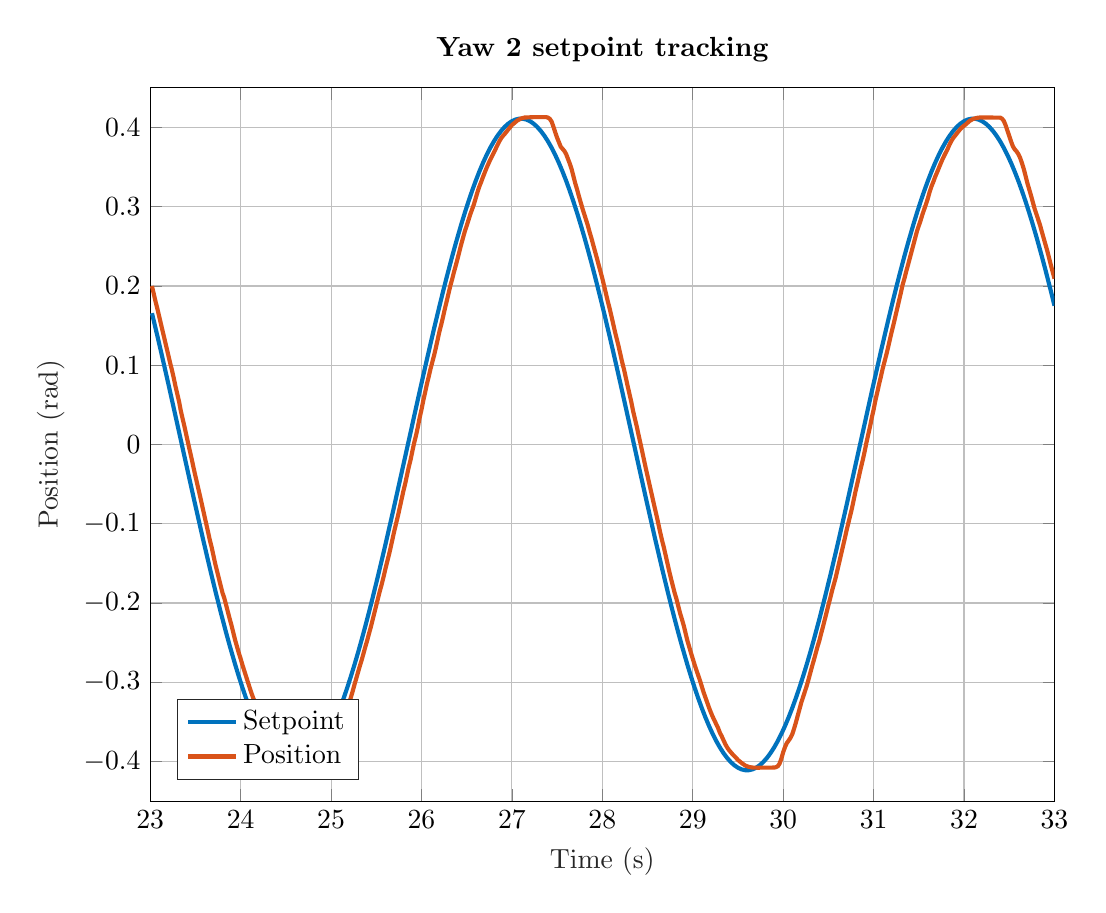
\begin{tikzpicture}

\begin{axis}[%
width=4.521in,
height=3.566in,
at={(0.758in,0.481in)},
scale only axis,
xmin=23,
xmax=33,
xlabel style={font=\color{white!15!black}},
xlabel={Time (s)},
ymin=-0.45,
ymax=0.45,
ylabel style={font=\color{white!15!black}},
ylabel={Position (rad)},
axis background/.style={fill=white},
title style={font=\bfseries},
title={Yaw 2 setpoint tracking},
xmajorgrids,
ymajorgrids,
legend style={at={(0.03,0.03)}, anchor=south west, legend cell align=left, align=left, draw=white!15!black}
]
\addplot [color=mycolor1, line width=1.5pt]
  table[row sep=crcr]{%
23.0191555	0.165668769531251\\
23.0791626	0.136850136718749\\
23.11917114	0.117195410156249\\
23.19929695	0.0770482421875016\\
23.3391819	0.00516695312499849\\
23.47919846	-0.0668738281249972\\
23.57920647	-0.117195410156249\\
23.65921402	-0.15615916015625\\
23.71923447	-0.1843680859375\\
23.77923203	-0.211529414062497\\
23.83923912	-0.237488769531247\\
23.87924385	-0.254054121093752\\
23.93925476	-0.277686171874997\\
23.9792614	-0.292572246093748\\
24.01925659	-0.306719218749997\\
24.05926514	-0.32009140625\\
24.09938622	-0.332655000000003\\
24.1392746	-0.344378320312501\\
24.17927551	-0.35523166015625\\
24.21928978	-0.36518767578125\\
24.25928879	-0.374221191406249\\
24.2994175	-0.382309394531248\\
24.33930206	-0.38943185546875\\
24.37930679	-0.395570585937499\\
24.41931152	-0.400710058593752\\
24.45931435	-0.404837304687497\\
24.49943924	-0.407941894531248\\
24.53932953	-0.410015976562498\\
24.57933235	-0.41105435546875\\
24.61933899	-0.41105435546875\\
24.65933609	-0.410015976562498\\
24.69947052	-0.407941894531248\\
24.73935127	-0.404837304687497\\
24.77935219	-0.400710058593752\\
24.81936455	-0.395570585937499\\
24.85939026	-0.38943185546875\\
24.89950562	-0.382309394531248\\
24.93938637	-0.374221191406249\\
24.97940445	-0.36518767578125\\
25.01939392	-0.35523166015625\\
25.05941391	-0.344378320312501\\
25.09952736	-0.332655000000003\\
25.13941765	-0.32009140625\\
25.17942429	-0.306719218749997\\
25.21941948	-0.292572246093748\\
25.2595253	-0.277686171874997\\
25.29954147	-0.262098671875002\\
25.33945274	-0.245849082031249\\
25.37944412	-0.228978476562503\\
25.41944885	-0.211529414062497\\
25.45945358	-0.193546015625003\\
25.51947403	-0.165668769531251\\
25.57947159	-0.136850136718749\\
25.61948204	-0.117195410156249\\
25.69965935	-0.0770482421875016\\
25.89969635	0.0258184765624989\\
25.95955086	0.0566571875000008\\
26.03957939	0.0972446484375027\\
26.09970474	0.127062910156248\\
26.13957214	0.146550937500002\\
26.17958832	0.165668769531251\\
26.23957825	0.193546015625003\\
26.27958679	0.211529414062497\\
26.33958435	0.237488769531247\\
26.37959862	0.254054121093752\\
26.43959999	0.277686171874997\\
26.47961998	0.292572246093748\\
26.51965904	0.306719218749997\\
26.559618	0.32009140625\\
26.59978867	0.332655000000003\\
26.63961983	0.344378320312501\\
26.67969131	0.35523166015625\\
26.71968079	0.36518767578125\\
26.7596817	0.374221191406249\\
26.79981041	0.382309394531248\\
26.83969688	0.38943185546875\\
26.8796978	0.395570585937499\\
26.91968918	0.400710058593752\\
26.95970345	0.404837304687497\\
26.9998188	0.407941894531248\\
27.03972244	0.410015976562498\\
27.07970428	0.41105435546875\\
27.11972046	0.41105435546875\\
27.15972137	0.410015976562498\\
27.19987488	0.407941894531248\\
27.23973846	0.404837304687497\\
27.27972794	0.400710058593752\\
27.31974983	0.395570585937499\\
27.3597641	0.38943185546875\\
27.39987946	0.382309394531248\\
27.43976212	0.374221191406249\\
27.47976685	0.36518767578125\\
27.51978683	0.35523166015625\\
27.55976677	0.344378320312501\\
27.59990501	0.332655000000003\\
27.63977814	0.32009140625\\
27.67980003	0.306719218749997\\
27.71977997	0.292572246093748\\
27.75979042	0.277686171874997\\
27.79992867	0.262098671875002\\
27.83981323	0.245849082031249\\
27.87981415	0.228978476562503\\
27.91983032	0.211529414062497\\
27.97982025	0.1843680859375\\
28.01981544	0.165668769531251\\
28.07985115	0.136850136718749\\
28.11987686	0.117195410156249\\
28.19997215	0.0770482421875016\\
28.31985855	0.0154976171874992\\
28.47991753	-0.0668738281249972\\
28.57987976	-0.117195410156249\\
28.65989304	-0.15615916015625\\
28.71993256	-0.1843680859375\\
28.75995255	-0.202601699218746\\
28.80004501	-0.220323515624997\\
28.8399334	-0.237488769531247\\
28.87992287	-0.254054121093752\\
28.93993759	-0.277686171874997\\
28.97994614	-0.292572246093748\\
29.01994705	-0.306719218749997\\
29.05997849	-0.32009140625\\
29.10009575	-0.332655000000003\\
29.13996696	-0.344378320312501\\
29.17998505	-0.35523166015625\\
29.21994209	-0.36518767578125\\
29.25997353	-0.374221191406249\\
29.30012321	-0.382309394531248\\
29.34000587	-0.38943185546875\\
29.3800087	-0.395570585937499\\
29.41999435	-0.400710058593752\\
29.46001816	-0.404837304687497\\
29.50014114	-0.407941894531248\\
29.54003143	-0.410015976562498\\
29.58001518	-0.41105435546875\\
29.62005615	-0.41105435546875\\
29.66002274	-0.410015976562498\\
29.70015717	-0.407941894531248\\
29.74006462	-0.404837304687497\\
29.78003311	-0.400710058593752\\
29.82004356	-0.395570585937499\\
29.86007118	-0.38943185546875\\
29.90019608	-0.382309394531248\\
29.94006538	-0.374221191406249\\
29.98004532	-0.36518767578125\\
30.02007484	-0.35523166015625\\
30.06008911	-0.344378320312501\\
30.10021591	-0.332655000000003\\
30.14009857	-0.32009140625\\
30.18009949	-0.306719218749997\\
30.22017097	-0.292572246093748\\
30.26011658	-0.277686171874997\\
30.30026627	-0.262098671875002\\
30.34012604	-0.245849082031249\\
30.40029907	-0.220323515624997\\
30.4601326	-0.193546015625003\\
30.52017593	-0.165668769531251\\
30.58013344	-0.136850136718749\\
30.62013245	-0.117195410156249\\
30.70029259	-0.0770482421875016\\
30.84021378	-0.00516695312499849\\
30.980196	0.0668738281249972\\
31.08020401	0.117195410156249\\
31.1602459	0.15615916015625\\
31.22019577	0.1843680859375\\
31.28022957	0.211529414062497\\
31.34022331	0.237488769531247\\
31.38021278	0.254054121093752\\
31.44024277	0.277686171874997\\
31.48025322	0.292572246093748\\
31.520298	0.306719218749997\\
31.56042099	0.32009140625\\
31.60041428	0.332655000000003\\
31.64028549	0.344378320312501\\
31.68028259	0.35523166015625\\
31.72029877	0.36518767578125\\
31.76030731	0.374221191406249\\
31.80044556	0.382309394531248\\
31.84035492	0.38943185546875\\
31.88029289	0.395570585937499\\
31.92034912	0.400710058593752\\
31.96029282	0.404837304687497\\
32.00043488	0.407941894531248\\
32.04032898	0.410015976562498\\
32.08035278	0.41105435546875\\
32.12031555	0.41105435546875\\
32.16034317	0.410015976562498\\
32.20049286	0.407941894531248\\
32.24038315	0.404837304687497\\
32.28037262	0.400710058593752\\
32.32038116	0.395570585937499\\
32.36040878	0.38943185546875\\
32.40048218	0.382309394531248\\
32.44039536	0.374221191406249\\
32.48039627	0.36518767578125\\
32.5204277	0.35523166015625\\
32.56040192	0.344378320312501\\
32.60052109	0.332655000000003\\
32.64037704	0.32009140625\\
32.68041992	0.306719218749997\\
32.72045135	0.292572246093748\\
32.7604332	0.277686171874997\\
32.8005867	0.262098671875002\\
32.86040115	0.237488769531247\\
32.90053558	0.220323515624997\\
32.96042633	0.193546015625003\\
33.00058746	0.175073710937497\\
};
\addlegendentry{Setpoint}

\addplot [color=mycolor2, line width=1.5pt]
  table[row sep=crcr]{%
23.0191555	0.199901718749999\\
23.05915833	0.180202187500001\\
23.0791626	0.171159785156249\\
23.1391716	0.142094921875\\
23.21917725	0.103341757812501\\
23.23917961	0.094299355468749\\
23.25918198	0.0842881250000005\\
23.27918243	0.073469531249998\\
23.31919098	0.0539314843749992\\
23.3391819	0.0418211132812516\\
23.37919235	0.0222830664062528\\
23.41919327	0.00145324218750176\\
23.459198	-0.0187307031250015\\
23.47919846	-0.0293878124999978\\
23.4993248	-0.0397219921875021\\
23.55920982	-0.0692712695312494\\
23.57920647	-0.0797669140625032\\
23.63921356	-0.110285039062497\\
23.65921402	-0.12078068359375\\
23.67922783	-0.129661601562503\\
23.71923447	-0.150814375000003\\
23.77923203	-0.178264531250001\\
23.79936218	-0.187306933593753\\
23.81923676	-0.193927265625\\
23.87924385	-0.220247128906252\\
23.89936638	-0.228482187499999\\
23.93925476	-0.247051386718752\\
23.9792614	-0.2630370703125\\
23.99937439	-0.270141835937501\\
24.01925659	-0.278053925781251\\
24.09938622	-0.306795839843751\\
24.11927795	-0.313739121093747\\
24.1392746	-0.320036523437501\\
24.15927696	-0.325526542968753\\
24.17927551	-0.331985390625\\
24.19940376	-0.337959843749999\\
24.21928978	-0.343288378906252\\
24.23929024	-0.348132539062497\\
24.25928879	-0.353784062499997\\
24.27929878	-0.358466718750002\\
24.2994175	-0.363633828125003\\
24.33930206	-0.37235328125\\
24.37930679	-0.381395683593752\\
24.39942551	-0.384948046875003\\
24.41931152	-0.387854531249999\\
24.47932053	-0.394313398437497\\
24.51931763	-0.399319023437499\\
24.55933571	-0.403678749999997\\
24.57933235	-0.405616386718748\\
24.61933899	-0.407554062499997\\
24.65933609	-0.408522871093751\\
24.89950562	-0.408199960937502\\
24.9193821	-0.407554062499997\\
24.93938637	-0.406100800781253\\
24.9593811	-0.401256699218749\\
24.97940445	-0.394313398437497\\
24.99950981	-0.386724257812503\\
25.01939392	-0.381234179687503\\
25.03940964	-0.376712988281248\\
25.05941391	-0.37429091796875\\
25.07941818	-0.3705770703125\\
25.09952736	-0.366055898437502\\
25.11941338	-0.359274062499999\\
25.13941765	-0.35120052734375\\
25.15943146	-0.342481074218753\\
25.19954681	-0.326172421875\\
25.21941948	-0.319067675781248\\
25.23942566	-0.311155566406249\\
25.2595253	-0.302759062500002\\
25.31944466	-0.279022753906247\\
25.33945274	-0.271595058593753\\
25.37944412	-0.255124960937501\\
25.39957237	-0.247212851562502\\
25.41944885	-0.238654863281248\\
25.43946648	-0.2304198046875\\
25.53948212	-0.184884882812497\\
25.55951691	-0.17664982421875\\
25.57947159	-0.167607421874997\\
25.59960938	-0.157596171874999\\
25.61948204	-0.148392304687498\\
25.63947678	-0.139511386718752\\
25.65950775	-0.129661601562503\\
25.69965935	-0.108831796875002\\
25.7395134	-0.0901010937500004\\
25.79967308	-0.0587756250000027\\
25.81952286	-0.049571757812501\\
25.85951996	-0.0282575195312518\\
25.87953758	-0.0192151171874997\\
25.89969635	-0.00807357421874855\\
25.91953659	0.00242207031249819\\
25.93952942	0.0114644726562503\\
25.95955086	0.021960117187497\\
25.97954559	0.0337475390625031\\
25.99969482	0.0437587695312516\\
26.01956367	0.0553847265625009\\
26.03957939	0.0653959570312495\\
26.05957413	0.0760530664062529\\
26.07955933	0.0854184179687465\\
26.09970474	0.0954296484375021\\
26.13957214	0.112545644531252\\
26.15955734	0.122395390625002\\
26.19974518	0.143225214843753\\
26.21959496	0.151944687499999\\
26.23957825	0.161632968749998\\
26.25958061	0.171805664062497\\
26.27958679	0.181171015624997\\
26.31958199	0.200547597656247\\
26.33958435	0.208782636718752\\
26.35961342	0.217825058593753\\
26.37959862	0.226060097656251\\
26.39978218	0.234779550781248\\
26.43959999	0.252702890625002\\
26.47961998	0.269172968749999\\
26.49975395	0.275954804687501\\
26.53966522	0.290487226562497\\
26.57962227	0.303081992187501\\
26.61962128	0.31858328125\\
26.63961983	0.325526542968753\\
26.65966988	0.331178046875003\\
26.67969131	0.337475410156252\\
26.71968079	0.348939902343751\\
26.7596817	0.359274062499999\\
26.79981041	0.368316484375001\\
26.85968971	0.382364492187499\\
26.8796978	0.386239824218748\\
26.89981651	0.389307792968751\\
26.91968918	0.391729882812498\\
26.95970345	0.397542832031249\\
26.9998188	0.40303287109375\\
27.05970955	0.40884583984375\\
27.09983826	0.411267890624998\\
27.1397171	0.4125596875\\
27.23973846	0.413044121093748\\
27.37975121	0.413044121093748\\
27.39987946	0.41239822265625\\
27.41974258	0.4107834765625\\
27.43976212	0.407231132812498\\
27.45976257	0.400772265625001\\
27.47976685	0.393667499999999\\
27.49986458	0.387047187500002\\
27.53976059	0.375744179687501\\
27.57977867	0.370415625\\
27.59990501	0.366378808593751\\
27.63977814	0.354429941406252\\
27.65979767	0.347648144531249\\
27.69993019	0.329724804687501\\
27.71977997	0.322135625000001\\
27.73979187	0.313739121093747\\
27.77978325	0.297914921874998\\
27.83981323	0.276277714843751\\
27.85980034	0.267719765625003\\
27.87981415	0.260130585937503\\
27.89992714	0.251572617187499\\
27.93980408	0.235102500000004\\
27.95985031	0.226383046875\\
27.99995804	0.209589999999999\\
28.05982971	0.180848066406249\\
28.07985115	0.171967148437503\\
28.09995842	0.162278847656253\\
28.13983154	0.142256386718749\\
28.17984009	0.123848632812503\\
28.21988106	0.1035032421875\\
28.23985672	0.0946223046874977\\
28.27983856	0.0737924804687466\\
28.31985855	0.0539314843749992\\
28.33985138	0.0423055273437498\\
28.37986183	0.0230904296874996\\
28.40002632	0.0122718359374971\\
28.41988564	0.00226060546874862\\
28.47991753	-0.0297107617187535\\
28.5398941	-0.0599059179687487\\
28.57987976	-0.0800898632812519\\
28.60004807	-0.0899396289062508\\
28.63990402	-0.110930917968751\\
28.65989304	-0.12078068359375\\
28.67989922	-0.129661601562503\\
28.73991013	-0.160018261718747\\
28.75995255	-0.169545058593748\\
28.80004501	-0.187468417968752\\
28.81992149	-0.195057558593753\\
28.85992241	-0.2129808984375\\
28.87992287	-0.220408593750001\\
28.90008354	-0.228482187499999\\
28.93993759	-0.247212851562502\\
28.97994614	-0.26287560546875\\
29.01994705	-0.277730976562502\\
29.03996849	-0.284674257812497\\
29.0799942	-0.297914921874998\\
29.11994553	-0.3127703125\\
29.17998505	-0.332146874999999\\
29.20013809	-0.338121308593749\\
29.21994209	-0.3434498828125\\
29.27997208	-0.357820859375003\\
29.30012321	-0.363795292968753\\
29.32001114	-0.368155019531251\\
29.36000061	-0.37816623046875\\
29.3800087	-0.382203046874999\\
29.40013885	-0.3855939453125\\
29.43998337	-0.390922500000002\\
29.48002243	-0.395605156249999\\
29.50014114	-0.398188710937497\\
29.54003143	-0.401902558593747\\
29.58001518	-0.405131992187499\\
29.62005615	-0.4069081640625\\
29.66002274	-0.407715527343747\\
29.720047	-0.407876992187497\\
29.90019608	-0.407715527343747\\
29.92011642	-0.407231132812498\\
29.94006538	-0.406100800781253\\
29.9600811	-0.402709902343751\\
29.98004532	-0.396412539062503\\
30.00018692	-0.388338925781248\\
30.02007484	-0.38188009765625\\
30.0401001	-0.376874492187497\\
30.08009148	-0.370415625\\
30.10021591	-0.365732929687503\\
30.12007904	-0.35878966796875\\
30.14009857	-0.351039023437501\\
30.20022011	-0.325688007812502\\
30.26011658	-0.304696699218752\\
30.28011322	-0.296623164062503\\
30.32013321	-0.279668632812502\\
30.34012604	-0.271756523437503\\
30.38015175	-0.254963496093751\\
30.40029907	-0.2475358203125\\
30.42012215	-0.238493398437498\\
30.44019699	-0.229935410156251\\
30.48015213	-0.211850585937498\\
30.50025749	-0.202646718750003\\
30.52017593	-0.194088749999999\\
30.54016113	-0.184723398437498\\
30.58013344	-0.168253300781252\\
30.68021393	-0.119165976562499\\
30.70029259	-0.108831796875002\\
30.76015854	-0.0807357421874997\\
30.80030251	-0.0589370898437522\\
30.82019997	-0.0492488085937524\\
30.8602047	-0.0289033984374996\\
30.88019753	-0.0196995312499979\\
30.90029144	-0.00920386718750166\\
30.92017746	0.00209912109374955\\
30.96017838	0.0224445312500023\\
30.980196	0.0339090234375021\\
31.00031853	0.0440817187500002\\
31.02017975	0.0557076757812496\\
31.04024887	0.065557421874999\\
31.06018448	0.0758916015625033\\
31.08020401	0.0854184179687465\\
31.10031509	0.0955911328125012\\
31.14019394	0.11303005859375\\
31.1602459	0.122395390625002\\
31.18021011	0.1325680859375\\
31.20035934	0.142417871093748\\
31.22019577	0.151460253906251\\
31.30033493	0.190859316406247\\
31.32023621	0.201193476562501\\
31.34022331	0.2091055859375\\
31.3602562	0.218147988281252\\
31.38021278	0.226383046875\\
31.48025322	0.269334472656247\\
31.520298	0.282898046874998\\
31.54026985	0.290325761718748\\
31.5802803	0.303566406249999\\
31.60041428	0.310671171875001\\
31.62028503	0.318906191406249\\
31.64028549	0.325688007812502\\
31.66029358	0.331339511718753\\
31.68028259	0.3376369140625\\
31.70036697	0.342965468750002\\
31.74024773	0.354107011718753\\
31.76030731	0.359435566406248\\
31.78029251	0.364279687500002\\
31.82031822	0.373322109375003\\
31.84035492	0.378650664062498\\
31.8602562	0.383010390625003\\
31.88029289	0.386724257812503\\
31.96029282	0.398188710937497\\
31.98027229	0.400449316406252\\
32.02036285	0.404001679687497\\
32.06033325	0.408199960937502\\
32.10045242	0.4107834765625\\
32.14030457	0.412075234375003\\
32.18030548	0.4127211328125\\
32.40048218	0.41239822265625\\
32.42037964	0.411106445312498\\
32.44039536	0.408199960937502\\
32.46037674	0.402709902343751\\
32.50051117	0.389146289062502\\
32.5204277	0.382364492187499\\
32.54035187	0.37622859375\\
32.56040192	0.372514746093749\\
32.58039856	0.369931191406252\\
32.60052109	0.3665403125\\
32.62041473	0.361696152343747\\
32.64037704	0.35523728515625\\
32.66038513	0.347809609374998\\
32.68041992	0.339090117187503\\
32.70054245	0.329886269531251\\
32.74040604	0.314385019531251\\
32.78042221	0.297591972656249\\
32.84041977	0.276923613281248\\
32.86040115	0.268527109375\\
32.92047119	0.244467832031248\\
32.96042633	0.226383046875\\
33.00058746	0.209267070312499\\
};
\addlegendentry{Position}

\end{axis}
\end{tikzpicture}%
		}
		\caption{Yaw 2 delay ~ 0.07 s}
	\end{subfigure}
	\begin{subfigure}[b]{0.5\textwidth}
		\centering
		\resizebox{\linewidth}{!}{
			% This file was created by matlab2tikz.
%
%The latest updates can be retrieved from
%  http://www.mathworks.com/matlabcentral/fileexchange/22022-matlab2tikz-matlab2tikz
%where you can also make suggestions and rate matlab2tikz.
%
\definecolor{mycolor1}{rgb}{0.00000,0.44700,0.74100}%
\definecolor{mycolor2}{rgb}{0.85000,0.32500,0.09800}%
%
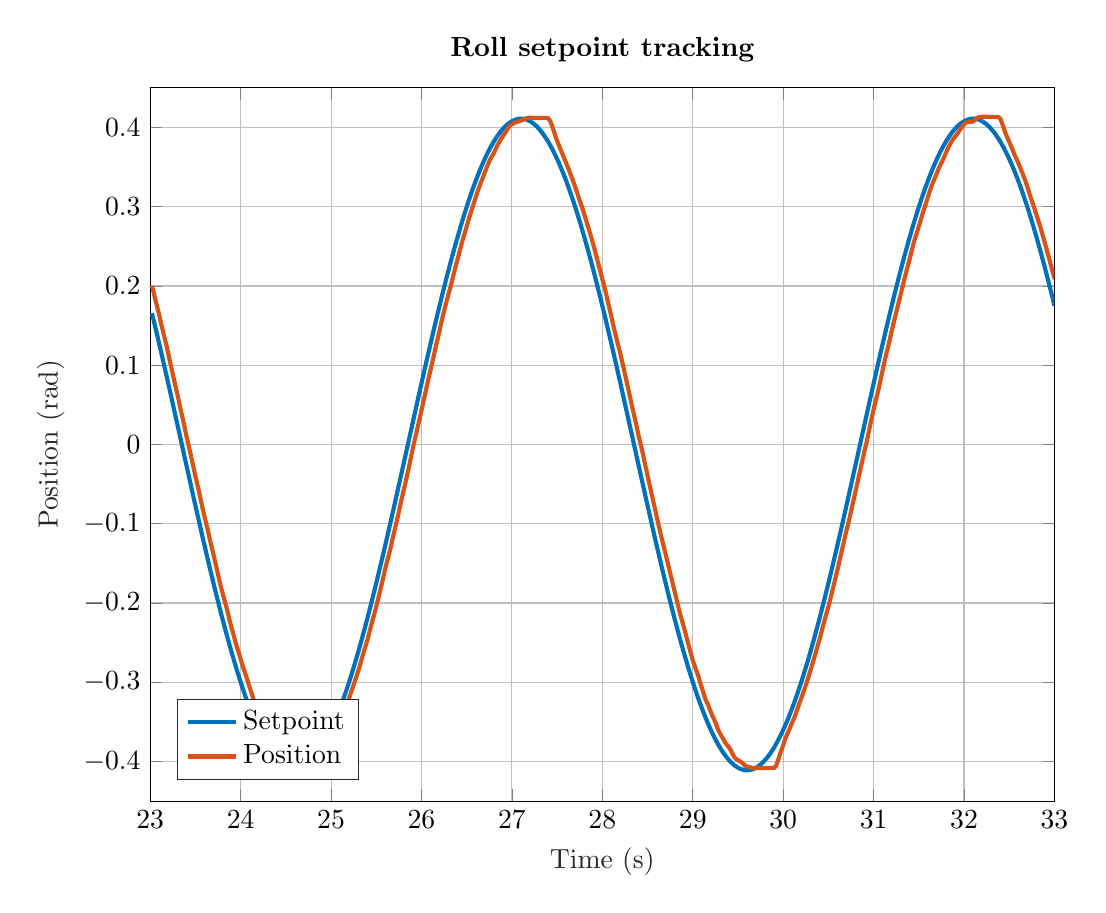
\begin{tikzpicture}

\begin{axis}[%
width=4.521in,
height=3.566in,
at={(0.758in,0.481in)},
scale only axis,
xmin=23,
xmax=33,
xlabel style={font=\color{white!15!black}},
xlabel={Time (s)},
ymin=-0.45,
ymax=0.45,
ylabel style={font=\color{white!15!black}},
ylabel={Position (rad)},
axis background/.style={fill=white},
title style={font=\bfseries},
title={Roll setpoint tracking},
xmajorgrids,
ymajorgrids,
legend style={at={(0.03,0.03)}, anchor=south west, legend cell align=left, align=left, draw=white!15!black}
]
\addplot [color=mycolor1, line width=1.5pt]
  table[row sep=crcr]{%
23.0191555	0.165668769531251\\
23.0791626	0.136850136718749\\
23.11917114	0.117195410156249\\
23.19929695	0.0770482421875016\\
23.3391819	0.00516695312499849\\
23.47919846	-0.0668738281249972\\
23.57920647	-0.117195410156249\\
23.65921402	-0.15615916015625\\
23.71923447	-0.1843680859375\\
23.77923203	-0.211529414062497\\
23.83923912	-0.237488769531247\\
23.87924385	-0.254054121093752\\
23.93925476	-0.277686171874997\\
23.9792614	-0.292572246093748\\
24.01925659	-0.306719218749997\\
24.05926514	-0.32009140625\\
24.09938622	-0.332655000000003\\
24.1392746	-0.344378320312501\\
24.17927551	-0.35523166015625\\
24.21928978	-0.36518767578125\\
24.25928879	-0.374221191406249\\
24.2994175	-0.382309394531248\\
24.33930206	-0.38943185546875\\
24.37930679	-0.395570585937499\\
24.41931152	-0.400710058593752\\
24.45931435	-0.404837304687497\\
24.49943924	-0.407941894531248\\
24.53932953	-0.410015976562498\\
24.57933235	-0.41105435546875\\
24.61933899	-0.41105435546875\\
24.65933609	-0.410015976562498\\
24.69947052	-0.407941894531248\\
24.73935127	-0.404837304687497\\
24.77935219	-0.400710058593752\\
24.81936455	-0.395570585937499\\
24.85939026	-0.38943185546875\\
24.89950562	-0.382309394531248\\
24.93938637	-0.374221191406249\\
24.97940445	-0.36518767578125\\
25.01939392	-0.35523166015625\\
25.05941391	-0.344378320312501\\
25.09952736	-0.332655000000003\\
25.13941765	-0.32009140625\\
25.17942429	-0.306719218749997\\
25.21941948	-0.292572246093748\\
25.2595253	-0.277686171874997\\
25.29954147	-0.262098671875002\\
25.33945274	-0.245849082031249\\
25.37944412	-0.228978476562503\\
25.41944885	-0.211529414062497\\
25.45945358	-0.193546015625003\\
25.51947403	-0.165668769531251\\
25.57947159	-0.136850136718749\\
25.61948204	-0.117195410156249\\
25.69965935	-0.0770482421875016\\
25.89969635	0.0258184765624989\\
25.95955086	0.0566571875000008\\
26.03957939	0.0972446484375027\\
26.09970474	0.127062910156248\\
26.13957214	0.146550937500002\\
26.17958832	0.165668769531251\\
26.23957825	0.193546015625003\\
26.27958679	0.211529414062497\\
26.33958435	0.237488769531247\\
26.37959862	0.254054121093752\\
26.43959999	0.277686171874997\\
26.47961998	0.292572246093748\\
26.51965904	0.306719218749997\\
26.559618	0.32009140625\\
26.59978867	0.332655000000003\\
26.63961983	0.344378320312501\\
26.67969131	0.35523166015625\\
26.71968079	0.36518767578125\\
26.7596817	0.374221191406249\\
26.79981041	0.382309394531248\\
26.83969688	0.38943185546875\\
26.8796978	0.395570585937499\\
26.91968918	0.400710058593752\\
26.95970345	0.404837304687497\\
26.9998188	0.407941894531248\\
27.03972244	0.410015976562498\\
27.07970428	0.41105435546875\\
27.11972046	0.41105435546875\\
27.15972137	0.410015976562498\\
27.19987488	0.407941894531248\\
27.23973846	0.404837304687497\\
27.27972794	0.400710058593752\\
27.31974983	0.395570585937499\\
27.3597641	0.38943185546875\\
27.39987946	0.382309394531248\\
27.43976212	0.374221191406249\\
27.47976685	0.36518767578125\\
27.51978683	0.35523166015625\\
27.55976677	0.344378320312501\\
27.59990501	0.332655000000003\\
27.63977814	0.32009140625\\
27.67980003	0.306719218749997\\
27.71977997	0.292572246093748\\
27.75979042	0.277686171874997\\
27.79992867	0.262098671875002\\
27.83981323	0.245849082031249\\
27.87981415	0.228978476562503\\
27.91983032	0.211529414062497\\
27.97982025	0.1843680859375\\
28.01981544	0.165668769531251\\
28.07985115	0.136850136718749\\
28.11987686	0.117195410156249\\
28.19997215	0.0770482421875016\\
28.31985855	0.0154976171874992\\
28.47991753	-0.0668738281249972\\
28.57987976	-0.117195410156249\\
28.65989304	-0.15615916015625\\
28.71993256	-0.1843680859375\\
28.75995255	-0.202601699218746\\
28.80004501	-0.220323515624997\\
28.8399334	-0.237488769531247\\
28.87992287	-0.254054121093752\\
28.93993759	-0.277686171874997\\
28.97994614	-0.292572246093748\\
29.01994705	-0.306719218749997\\
29.05997849	-0.32009140625\\
29.10009575	-0.332655000000003\\
29.13996696	-0.344378320312501\\
29.17998505	-0.35523166015625\\
29.21994209	-0.36518767578125\\
29.25997353	-0.374221191406249\\
29.30012321	-0.382309394531248\\
29.34000587	-0.38943185546875\\
29.3800087	-0.395570585937499\\
29.41999435	-0.400710058593752\\
29.46001816	-0.404837304687497\\
29.50014114	-0.407941894531248\\
29.54003143	-0.410015976562498\\
29.58001518	-0.41105435546875\\
29.62005615	-0.41105435546875\\
29.66002274	-0.410015976562498\\
29.70015717	-0.407941894531248\\
29.74006462	-0.404837304687497\\
29.78003311	-0.400710058593752\\
29.82004356	-0.395570585937499\\
29.86007118	-0.38943185546875\\
29.90019608	-0.382309394531248\\
29.94006538	-0.374221191406249\\
29.98004532	-0.36518767578125\\
30.02007484	-0.35523166015625\\
30.06008911	-0.344378320312501\\
30.10021591	-0.332655000000003\\
30.14009857	-0.32009140625\\
30.18009949	-0.306719218749997\\
30.22017097	-0.292572246093748\\
30.26011658	-0.277686171874997\\
30.30026627	-0.262098671875002\\
30.34012604	-0.245849082031249\\
30.40029907	-0.220323515624997\\
30.4601326	-0.193546015625003\\
30.52017593	-0.165668769531251\\
30.58013344	-0.136850136718749\\
30.62013245	-0.117195410156249\\
30.70029259	-0.0770482421875016\\
30.84021378	-0.00516695312499849\\
30.980196	0.0668738281249972\\
31.08020401	0.117195410156249\\
31.1602459	0.15615916015625\\
31.22019577	0.1843680859375\\
31.28022957	0.211529414062497\\
31.34022331	0.237488769531247\\
31.38021278	0.254054121093752\\
31.44024277	0.277686171874997\\
31.48025322	0.292572246093748\\
31.520298	0.306719218749997\\
31.56042099	0.32009140625\\
31.60041428	0.332655000000003\\
31.64028549	0.344378320312501\\
31.68028259	0.35523166015625\\
31.72029877	0.36518767578125\\
31.76030731	0.374221191406249\\
31.80044556	0.382309394531248\\
31.84035492	0.38943185546875\\
31.88029289	0.395570585937499\\
31.92034912	0.400710058593752\\
31.96029282	0.404837304687497\\
32.00043488	0.407941894531248\\
32.04032898	0.410015976562498\\
32.08035278	0.41105435546875\\
32.12031555	0.41105435546875\\
32.16034317	0.410015976562498\\
32.20049286	0.407941894531248\\
32.24038315	0.404837304687497\\
32.28037262	0.400710058593752\\
32.32038116	0.395570585937499\\
32.36040878	0.38943185546875\\
32.40048218	0.382309394531248\\
32.44039536	0.374221191406249\\
32.48039627	0.36518767578125\\
32.5204277	0.35523166015625\\
32.56040192	0.344378320312501\\
32.60052109	0.332655000000003\\
32.64037704	0.32009140625\\
32.68041992	0.306719218749997\\
32.72045135	0.292572246093748\\
32.7604332	0.277686171874997\\
32.8005867	0.262098671875002\\
32.86040115	0.237488769531247\\
32.90053558	0.220323515624997\\
32.96042633	0.193546015625003\\
33.00058746	0.175073710937497\\
};
\addlegendentry{Setpoint}

\addplot [color=mycolor2, line width=1.5pt]
  table[row sep=crcr]{%
23.0191555	0.200063183593748\\
23.03915405	0.191505195312502\\
23.05915833	0.181332500000003\\
23.0992794	0.163247695312499\\
23.11917114	0.153074980468752\\
23.15916443	0.134182812500001\\
23.17917252	0.125140410156249\\
23.19929695	0.114806230468751\\
23.21917725	0.104149121093748\\
23.27918243	0.0737924804687466\\
23.29930305	0.0639427148437477\\
23.31919098	0.0529626562500027\\
23.3391819	0.0426284765624985\\
23.35918236	0.0327787109374995\\
23.37919235	0.0222830664062528\\
23.39931488	0.0111415234375016\\
23.41919327	0.00161470703125133\\
23.43920135	-0.00839652343749719\\
23.4993248	-0.0398834570312516\\
23.53920555	-0.0595829882812495\\
23.57920647	-0.0807357421874997\\
23.63921356	-0.1093162109375\\
23.65921402	-0.119650371093748\\
23.69934082	-0.138865488281247\\
23.77923203	-0.178748945312499\\
23.83923912	-0.203777031249999\\
23.87924385	-0.222507714843751\\
23.89936638	-0.231227187499996\\
23.91924667	-0.239462226562502\\
23.93925476	-0.248181699218748\\
23.95925522	-0.255770859374998\\
23.9792614	-0.26287560546875\\
24.01925659	-0.278215390625\\
24.05926514	-0.291940468749999\\
24.1392746	-0.32052091796875\\
24.21928978	-0.343934277343749\\
24.23929024	-0.34910138671875\\
24.25928879	-0.354914375\\
24.27929878	-0.361211738281249\\
24.2994175	-0.364925605468748\\
24.33930206	-0.374129453125001\\
24.35929871	-0.377843300781251\\
24.39942551	-0.383979238281249\\
24.4393177	-0.39156837890625\\
24.45931435	-0.394636367187502\\
24.47932053	-0.396896933593752\\
24.53932953	-0.399641953124998\\
24.55933571	-0.402225507812503\\
24.57933235	-0.405293457031249\\
24.59946823	-0.4069081640625\\
24.61933899	-0.407876992187497\\
24.67933464	-0.408038476562503\\
24.87937546	-0.407715527343747\\
24.89950562	-0.407554062499997\\
24.9193821	-0.404001679687497\\
24.9593811	-0.392214277343747\\
24.99950981	-0.379296582031252\\
25.03940964	-0.367024707031248\\
25.05941391	-0.362180546875003\\
25.07941818	-0.356851992187501\\
25.11941338	-0.345064589843751\\
25.13941765	-0.338282792968748\\
25.15943146	-0.332469824218748\\
25.17942429	-0.326172421875\\
25.19954681	-0.320197988281251\\
25.21941948	-0.313093222656249\\
25.23942566	-0.306795839843751\\
25.27942657	-0.293232246093751\\
25.31944466	-0.278861289062498\\
25.33945274	-0.270303281250001\\
25.37944412	-0.254963496093751\\
25.39957237	-0.2475358203125\\
25.41944885	-0.238977812500003\\
25.43946648	-0.229773945312502\\
25.47947884	-0.213465312499999\\
25.49957657	-0.204584394531253\\
25.55951691	-0.17648833984375\\
25.57947159	-0.166800058593751\\
25.59960938	-0.156465878906253\\
25.61948204	-0.147423476562501\\
25.63947678	-0.139349902343753\\
25.65950775	-0.129984570312502\\
25.67949295	-0.119327421874999\\
25.71951675	-0.100112324218749\\
25.7395134	-0.0904240429687491\\
25.77954102	-0.0691098046874998\\
25.81952286	-0.0498946875000001\\
25.83953857	-0.0392375781249967\\
25.85951996	-0.0295492773437473\\
25.89969635	-0.00710474609375211\\
25.97954559	0.0327787109374995\\
26.07955933	0.0841266601562509\\
26.11956024	0.1035032421875\\
26.13957214	0.113998886718747\\
26.17958832	0.133536933593753\\
26.19974518	0.143709628906251\\
26.21959496	0.154366757812497\\
26.23957825	0.163893574218747\\
26.29973793	0.190536367187498\\
26.31958199	0.198125527343748\\
26.37959862	0.225737148437503\\
26.39978218	0.234133671875\\
26.43959999	0.251572617187499\\
26.45960236	0.259969121093754\\
26.47961998	0.267235332031248\\
26.49975395	0.274985937499999\\
26.51965904	0.283059550781253\\
26.53966522	0.290648691406247\\
26.61962128	0.318906191406249\\
26.65966988	0.331500976562502\\
26.67969131	0.336829550781253\\
26.69979858	0.342803984375003\\
26.71968079	0.3492628515625\\
26.7596817	0.359758496093747\\
26.77966881	0.363795292968753\\
26.79981041	0.367509121093747\\
26.81968689	0.372676230468748\\
26.83969688	0.377520371093752\\
26.8796978	0.3855939453125\\
26.91968918	0.392214277343747\\
26.95970345	0.399641953124998\\
26.97970009	0.402548437500002\\
27.01970673	0.405293457031249\\
27.05970955	0.407231132812498\\
27.07970428	0.407715527343747\\
27.09983826	0.40884583984375\\
27.11972046	0.409330234374998\\
27.1397171	0.410299082031251\\
27.15972137	0.411752324218753\\
27.17972946	0.412236757812501\\
27.37975121	0.412075234375003\\
27.39987946	0.411752324218753\\
27.41974258	0.408684375\\
27.43976212	0.403355800781249\\
27.45976257	0.396896933593752\\
27.47976685	0.389469238281251\\
27.49986458	0.383010390625003\\
27.57977867	0.360565839843751\\
27.59990501	0.35523728515625\\
27.63977814	0.34361134765625\\
27.67980003	0.331662441406252\\
27.71977997	0.318260312500001\\
27.73979187	0.311155566406249\\
27.77978325	0.298076406249997\\
27.87981415	0.260453535156252\\
27.89992714	0.252379941406247\\
27.93980408	0.235263964843753\\
27.99995804	0.208459687500003\\
28.01981544	0.200224667968747\\
28.03981781	0.191343730468752\\
28.05982971	0.181009550781248\\
28.09995842	0.16131001953125\\
28.11987686	0.151137304687502\\
28.13983154	0.141449023437502\\
28.19997215	0.113998886718747\\
28.23985672	0.0941378906249994\\
28.27983856	0.073469531249998\\
28.3000145	0.0634583007812495\\
28.31985855	0.052639707031247\\
28.37986183	0.022767480468751\\
28.40002632	0.0114644726562503\\
28.41988564	0.00226060546874862\\
28.43987274	-0.00742769531250076\\
28.45988464	-0.0184077539062528\\
28.51988983	-0.049571757812501\\
28.57987976	-0.080251347656251\\
28.61990929	-0.100596738281247\\
28.65989304	-0.119973320312504\\
28.67989922	-0.129015722656249\\
28.8399334	-0.204584394531253\\
28.85992241	-0.213626796874998\\
28.91993523	-0.23817044921875\\
28.93993759	-0.247374316406251\\
29.00005722	-0.272402421875\\
29.01994705	-0.279184199218747\\
29.05997849	-0.29177900390625\\
29.0799942	-0.299691113281249\\
29.13996696	-0.321489765625003\\
29.15997696	-0.32633388671875\\
29.17998505	-0.331662441406252\\
29.20013809	-0.33779837890625\\
29.21994209	-0.343126933593751\\
29.23999405	-0.347809609374998\\
29.25997353	-0.353622578124998\\
29.27997208	-0.359919960937503\\
29.30012321	-0.36444119140625\\
29.34000587	-0.372191796875001\\
29.36000061	-0.376551523437499\\
29.3800087	-0.379619472656252\\
29.40013885	-0.38188009765625\\
29.41999435	-0.385916874999999\\
29.46001816	-0.394797792968753\\
29.48002243	-0.3970584375\\
29.5200119	-0.399641953124998\\
29.54003143	-0.4010951953125\\
29.58001518	-0.405454921874998\\
29.60014915	-0.406423750000002\\
29.62005615	-0.406746699218751\\
29.66002274	-0.408361425781251\\
29.90019608	-0.408038476562503\\
29.92011642	-0.405939355468753\\
29.94006538	-0.399480488281249\\
29.98004532	-0.38575541015625\\
30.00018692	-0.379296582031252\\
30.02007484	-0.372514746093749\\
30.0401001	-0.366701777343749\\
30.06008911	-0.361857617187503\\
30.08009148	-0.356044648437504\\
30.12007904	-0.345710468749999\\
30.14009857	-0.33973603515625\\
30.18009949	-0.326010957031251\\
30.20022011	-0.320359453125\\
30.26011658	-0.300498437500003\\
30.32013321	-0.27837685546875\\
30.34012604	-0.270303281250001\\
30.36011124	-0.262714140625\\
30.38015175	-0.254479082031253\\
30.40029907	-0.246728457031253\\
30.42012215	-0.238331933593749\\
30.44019699	-0.229128046874997\\
30.50025749	-0.204422910156246\\
30.52017593	-0.19570345703125\\
30.60030365	-0.158242070312497\\
30.62013245	-0.148069355468749\\
30.70029259	-0.108347363281247\\
30.7202034	-0.0994664453125012\\
30.74013329	-0.0897781640625013\\
30.80030251	-0.0589370898437522\\
30.82019997	-0.0489258593749966\\
30.84021378	-0.0381072656250012\\
30.8602047	-0.0284189843750013\\
30.90029144	-0.00758916015625033\\
30.92017746	0.00161470703125133\\
30.94021988	0.0122718359374971\\
30.96017838	0.0234133593749988\\
31.00031853	0.0445661328124984\\
31.02017975	0.0539314843749992\\
31.04024887	0.0626509375000026\\
31.06018448	0.072339238281252\\
31.10031509	0.0941378906249994\\
31.14019394	0.114321816406253\\
31.1602459	0.123202753906249\\
31.20035934	0.143225214843753\\
31.22019577	0.152752031250003\\
31.32023621	0.198932871093753\\
31.34022331	0.208459687500003\\
31.38021278	0.226221562500001\\
31.40035629	0.234779550781248\\
31.42024994	0.24366048828125\\
31.44024277	0.253025820312502\\
31.46025085	0.260776464843751\\
31.48025322	0.267719765625003\\
31.50040054	0.275631835937503\\
31.54026985	0.290648691406247\\
31.5802803	0.304696699218752\\
31.60041428	0.312285878906252\\
31.62028503	0.319390644531254\\
31.64028549	0.325849492187501\\
31.66029358	0.331662441406252\\
31.70036697	0.342319570312497\\
31.72029877	0.348294042968753\\
31.74024773	0.35329962890625\\
31.76030731	0.357659355468748\\
31.78029251	0.362987929687499\\
31.80044556	0.367993554687502\\
31.82031822	0.373322109375003\\
31.8602562	0.3820415625\\
31.88029289	0.3855939453125\\
31.90040207	0.388177480468748\\
31.94027901	0.394313398437497\\
31.96029282	0.398188710937497\\
31.98027229	0.401256699218749\\
32.02036285	0.406100800781253\\
32.04032898	0.406746699218751\\
32.08035278	0.4069081640625\\
32.10045242	0.407715527343747\\
32.12031555	0.409330234374998\\
32.14030457	0.411752324218753\\
32.16034317	0.41288259765625\\
32.20049286	0.413528496093747\\
32.36040878	0.413367031249997\\
32.38039017	0.413044121093748\\
32.40048218	0.411267890624998\\
32.42037964	0.405616386718748\\
32.46037674	0.392214277343747\\
32.54035187	0.371222968749997\\
32.56040192	0.365248535156248\\
32.60052109	0.35523728515625\\
32.64037704	0.343934277343749\\
32.68041992	0.331985390625\\
32.70054245	0.325203613281253\\
32.74040604	0.310671171875001\\
32.78042221	0.297269023437501\\
32.84041977	0.275793320312502\\
32.90053558	0.251734082031248\\
32.98042679	0.217825058593753\\
33.00058746	0.208782636718752\\
};
\addlegendentry{Position}

\end{axis}
\end{tikzpicture}%
		}
		\caption{Roll delay ~ 0.06 s}
	\end{subfigure}
	\begin{subfigure}[b]{0.5\textwidth}
		\centering
		\resizebox{\linewidth}{!}{
			% This file was created by matlab2tikz.
%
%The latest updates can be retrieved from
%  http://www.mathworks.com/matlabcentral/fileexchange/22022-matlab2tikz-matlab2tikz
%where you can also make suggestions and rate matlab2tikz.
%
\definecolor{mycolor1}{rgb}{0.00000,0.44700,0.74100}%
\definecolor{mycolor2}{rgb}{0.85000,0.32500,0.09800}%
%
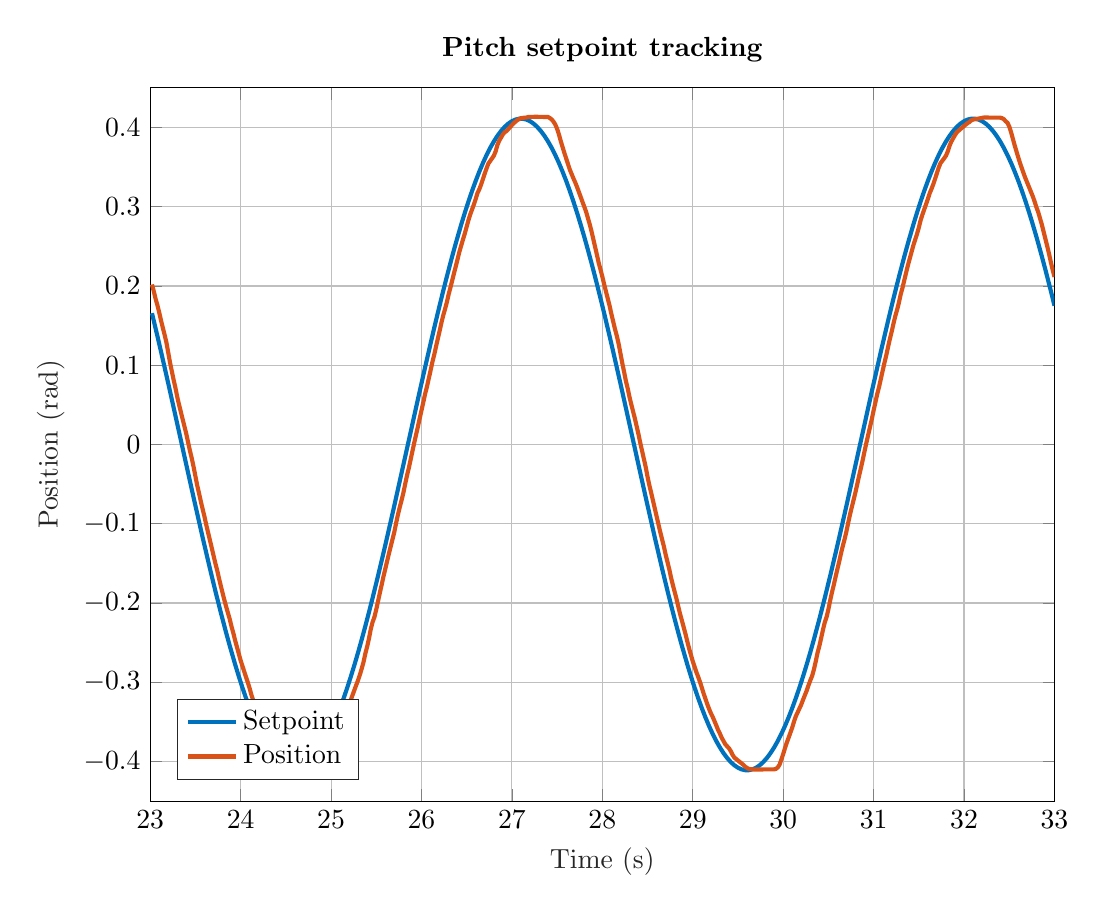
\begin{tikzpicture}

\begin{axis}[%
width=4.521in,
height=3.566in,
at={(0.758in,0.481in)},
scale only axis,
xmin=23,
xmax=33,
xlabel style={font=\color{white!15!black}},
xlabel={Time (s)},
ymin=-0.45,
ymax=0.45,
ylabel style={font=\color{white!15!black}},
ylabel={Position (rad)},
axis background/.style={fill=white},
title style={font=\bfseries},
title={Pitch setpoint tracking},
xmajorgrids,
ymajorgrids,
legend style={at={(0.03,0.03)}, anchor=south west, legend cell align=left, align=left, draw=white!15!black}
]
\addplot [color=mycolor1, line width=1.5pt]
  table[row sep=crcr]{%
23.0191555	0.165668769531251\\
23.0791626	0.136850136718749\\
23.11917114	0.117195410156249\\
23.19929695	0.0770482421875016\\
23.3391819	0.00516695312499849\\
23.47919846	-0.0668738281249972\\
23.57920647	-0.117195410156249\\
23.65921402	-0.15615916015625\\
23.71923447	-0.1843680859375\\
23.77923203	-0.211529414062497\\
23.83923912	-0.237488769531247\\
23.87924385	-0.254054121093752\\
23.93925476	-0.277686171874997\\
23.9792614	-0.292572246093748\\
24.01925659	-0.306719218749997\\
24.05926514	-0.32009140625\\
24.09938622	-0.332655000000003\\
24.1392746	-0.344378320312501\\
24.17927551	-0.35523166015625\\
24.21928978	-0.36518767578125\\
24.25928879	-0.374221191406249\\
24.2994175	-0.382309394531248\\
24.33930206	-0.38943185546875\\
24.37930679	-0.395570585937499\\
24.41931152	-0.400710058593752\\
24.45931435	-0.404837304687497\\
24.49943924	-0.407941894531248\\
24.53932953	-0.410015976562498\\
24.57933235	-0.41105435546875\\
24.61933899	-0.41105435546875\\
24.65933609	-0.410015976562498\\
24.69947052	-0.407941894531248\\
24.73935127	-0.404837304687497\\
24.77935219	-0.400710058593752\\
24.81936455	-0.395570585937499\\
24.85939026	-0.38943185546875\\
24.89950562	-0.382309394531248\\
24.93938637	-0.374221191406249\\
24.97940445	-0.36518767578125\\
25.01939392	-0.35523166015625\\
25.05941391	-0.344378320312501\\
25.09952736	-0.332655000000003\\
25.13941765	-0.32009140625\\
25.17942429	-0.306719218749997\\
25.21941948	-0.292572246093748\\
25.2595253	-0.277686171874997\\
25.29954147	-0.262098671875002\\
25.33945274	-0.245849082031249\\
25.37944412	-0.228978476562503\\
25.41944885	-0.211529414062497\\
25.45945358	-0.193546015625003\\
25.51947403	-0.165668769531251\\
25.57947159	-0.136850136718749\\
25.61948204	-0.117195410156249\\
25.69965935	-0.0770482421875016\\
25.89969635	0.0258184765624989\\
25.95955086	0.0566571875000008\\
26.03957939	0.0972446484375027\\
26.09970474	0.127062910156248\\
26.13957214	0.146550937500002\\
26.17958832	0.165668769531251\\
26.23957825	0.193546015625003\\
26.27958679	0.211529414062497\\
26.33958435	0.237488769531247\\
26.37959862	0.254054121093752\\
26.43959999	0.277686171874997\\
26.47961998	0.292572246093748\\
26.51965904	0.306719218749997\\
26.559618	0.32009140625\\
26.59978867	0.332655000000003\\
26.63961983	0.344378320312501\\
26.67969131	0.35523166015625\\
26.71968079	0.36518767578125\\
26.7596817	0.374221191406249\\
26.79981041	0.382309394531248\\
26.83969688	0.38943185546875\\
26.8796978	0.395570585937499\\
26.91968918	0.400710058593752\\
26.95970345	0.404837304687497\\
26.9998188	0.407941894531248\\
27.03972244	0.410015976562498\\
27.07970428	0.41105435546875\\
27.11972046	0.41105435546875\\
27.15972137	0.410015976562498\\
27.19987488	0.407941894531248\\
27.23973846	0.404837304687497\\
27.27972794	0.400710058593752\\
27.31974983	0.395570585937499\\
27.3597641	0.38943185546875\\
27.39987946	0.382309394531248\\
27.43976212	0.374221191406249\\
27.47976685	0.36518767578125\\
27.51978683	0.35523166015625\\
27.55976677	0.344378320312501\\
27.59990501	0.332655000000003\\
27.63977814	0.32009140625\\
27.67980003	0.306719218749997\\
27.71977997	0.292572246093748\\
27.75979042	0.277686171874997\\
27.79992867	0.262098671875002\\
27.83981323	0.245849082031249\\
27.87981415	0.228978476562503\\
27.91983032	0.211529414062497\\
27.97982025	0.1843680859375\\
28.01981544	0.165668769531251\\
28.07985115	0.136850136718749\\
28.11987686	0.117195410156249\\
28.19997215	0.0770482421875016\\
28.31985855	0.0154976171874992\\
28.47991753	-0.0668738281249972\\
28.57987976	-0.117195410156249\\
28.65989304	-0.15615916015625\\
28.71993256	-0.1843680859375\\
28.75995255	-0.202601699218746\\
28.80004501	-0.220323515624997\\
28.8399334	-0.237488769531247\\
28.87992287	-0.254054121093752\\
28.93993759	-0.277686171874997\\
28.97994614	-0.292572246093748\\
29.01994705	-0.306719218749997\\
29.05997849	-0.32009140625\\
29.10009575	-0.332655000000003\\
29.13996696	-0.344378320312501\\
29.17998505	-0.35523166015625\\
29.21994209	-0.36518767578125\\
29.25997353	-0.374221191406249\\
29.30012321	-0.382309394531248\\
29.34000587	-0.38943185546875\\
29.3800087	-0.395570585937499\\
29.41999435	-0.400710058593752\\
29.46001816	-0.404837304687497\\
29.50014114	-0.407941894531248\\
29.54003143	-0.410015976562498\\
29.58001518	-0.41105435546875\\
29.62005615	-0.41105435546875\\
29.66002274	-0.410015976562498\\
29.70015717	-0.407941894531248\\
29.74006462	-0.404837304687497\\
29.78003311	-0.400710058593752\\
29.82004356	-0.395570585937499\\
29.86007118	-0.38943185546875\\
29.90019608	-0.382309394531248\\
29.94006538	-0.374221191406249\\
29.98004532	-0.36518767578125\\
30.02007484	-0.35523166015625\\
30.06008911	-0.344378320312501\\
30.10021591	-0.332655000000003\\
30.14009857	-0.32009140625\\
30.18009949	-0.306719218749997\\
30.22017097	-0.292572246093748\\
30.26011658	-0.277686171874997\\
30.30026627	-0.262098671875002\\
30.34012604	-0.245849082031249\\
30.40029907	-0.220323515624997\\
30.4601326	-0.193546015625003\\
30.52017593	-0.165668769531251\\
30.58013344	-0.136850136718749\\
30.62013245	-0.117195410156249\\
30.70029259	-0.0770482421875016\\
30.84021378	-0.00516695312499849\\
30.980196	0.0668738281249972\\
31.08020401	0.117195410156249\\
31.1602459	0.15615916015625\\
31.22019577	0.1843680859375\\
31.28022957	0.211529414062497\\
31.34022331	0.237488769531247\\
31.38021278	0.254054121093752\\
31.44024277	0.277686171874997\\
31.48025322	0.292572246093748\\
31.520298	0.306719218749997\\
31.56042099	0.32009140625\\
31.60041428	0.332655000000003\\
31.64028549	0.344378320312501\\
31.68028259	0.35523166015625\\
31.72029877	0.36518767578125\\
31.76030731	0.374221191406249\\
31.80044556	0.382309394531248\\
31.84035492	0.38943185546875\\
31.88029289	0.395570585937499\\
31.92034912	0.400710058593752\\
31.96029282	0.404837304687497\\
32.00043488	0.407941894531248\\
32.04032898	0.410015976562498\\
32.08035278	0.41105435546875\\
32.12031555	0.41105435546875\\
32.16034317	0.410015976562498\\
32.20049286	0.407941894531248\\
32.24038315	0.404837304687497\\
32.28037262	0.400710058593752\\
32.32038116	0.395570585937499\\
32.36040878	0.38943185546875\\
32.40048218	0.382309394531248\\
32.44039536	0.374221191406249\\
32.48039627	0.36518767578125\\
32.5204277	0.35523166015625\\
32.56040192	0.344378320312501\\
32.60052109	0.332655000000003\\
32.64037704	0.32009140625\\
32.68041992	0.306719218749997\\
32.72045135	0.292572246093748\\
32.7604332	0.277686171874997\\
32.8005867	0.262098671875002\\
32.86040115	0.237488769531247\\
32.90053558	0.220323515624997\\
32.96042633	0.193546015625003\\
33.00058746	0.175073710937497\\
};
\addlegendentry{Setpoint}

\addplot [color=mycolor2, line width=1.5pt]
  table[row sep=crcr]{%
23.0191555	0.201839374999999\\
23.03915405	0.193442851562502\\
23.05915833	0.183916035156251\\
23.0791626	0.175842460937503\\
23.0992794	0.166477109375002\\
23.11917114	0.156627363281252\\
23.1391716	0.147262011718752\\
23.15916443	0.138381074218749\\
23.17917252	0.128531328125\\
23.21917725	0.103180273437502\\
23.25918198	0.0812201562499979\\
23.27918243	0.0712089257812494\\
23.29930305	0.0597444531249991\\
23.31919098	0.0498946875000001\\
23.37919235	0.0224445312500023\\
23.39931488	0.0130791992187511\\
23.41919327	0.00242207031249819\\
23.43920135	-0.00791210937499898\\
23.459198	-0.0174389257812493\\
23.47919846	-0.0280960351562527\\
23.51920509	-0.0515093945312515\\
23.53920555	-0.0613591601562504\\
23.55920982	-0.0716933593749971\\
23.57920647	-0.081381640624997\\
23.59934044	-0.0907469726562482\\
23.6192131	-0.101242636718752\\
23.67922783	-0.129984570312502\\
23.71923447	-0.149522597656251\\
23.73923111	-0.158242070312497\\
23.75923157	-0.168253300781252\\
23.77923203	-0.177780117187503\\
23.81923676	-0.196026386718749\\
23.83923912	-0.204584394531253\\
23.87924385	-0.220408593750001\\
23.89936638	-0.229935410156251\\
23.91924667	-0.23817044921875\\
23.93925476	-0.247374316406251\\
23.99937439	-0.272402421875\\
24.05926514	-0.29355517578125\\
24.07927322	-0.300337011718753\\
24.09938622	-0.307764687499997\\
24.11927795	-0.316161191406252\\
24.1392746	-0.322943007812498\\
24.15927696	-0.329078906249997\\
24.17927551	-0.334407460937499\\
24.19940376	-0.339413085937501\\
24.21928978	-0.343934277343749\\
24.27929878	-0.361696152343747\\
24.2994175	-0.365409999999997\\
24.31929207	-0.369931191406252\\
24.33930206	-0.373483574218753\\
24.35929871	-0.377843300781251\\
24.37930679	-0.380265390624999\\
24.39942551	-0.382203046874999\\
24.41931152	-0.385916874999999\\
24.4393177	-0.390438105468753\\
24.45931435	-0.394474863281253\\
24.49943924	-0.398511640625003\\
24.55933571	-0.40303287109375\\
24.57933235	-0.405293457031249\\
24.59946823	-0.4069081640625\\
24.63933563	-0.40884583984375\\
24.65933609	-0.409814648437496\\
24.71936226	-0.409976152343752\\
24.89950562	-0.409814648437496\\
24.9193821	-0.409491738281247\\
24.93938637	-0.407715527343747\\
24.9593811	-0.404647578125001\\
24.97940445	-0.398188710937497\\
25.01939392	-0.383494804687501\\
25.03940964	-0.376551523437499\\
25.07941818	-0.363310878906248\\
25.09952736	-0.356367578125003\\
25.13941765	-0.343934277343749\\
25.15943146	-0.338444257812498\\
25.17942429	-0.33392306640625\\
25.19954681	-0.32811009765625\\
25.2595253	-0.309379394531248\\
25.29954147	-0.297107558593751\\
25.31944466	-0.290325761718748\\
25.33945274	-0.282575136718748\\
25.35944366	-0.274340078125\\
25.37944412	-0.263682949218747\\
25.39957237	-0.254802031250001\\
25.41944885	-0.244629335937503\\
25.43946648	-0.232841894531248\\
25.45945358	-0.223960976562502\\
25.47947884	-0.217825058593753\\
25.49957657	-0.208298242187503\\
25.53948212	-0.187145449218747\\
25.55951691	-0.177134238281248\\
25.57947159	-0.166638574218752\\
25.61948204	-0.147423476562501\\
25.63947678	-0.137735195312501\\
25.69965935	-0.110285039062497\\
25.71951675	-0.0991434960937525\\
25.7395134	-0.0886478515624987\\
25.7595253	-0.0791210351562484\\
25.77954102	-0.0704015625000025\\
25.79967308	-0.0610362304687513\\
25.81952286	-0.0498946875000001\\
25.83953857	-0.0392375781249967\\
25.85951996	-0.0298722265625031\\
25.91953659	0.00209912109374955\\
25.95955086	0.0221216015625032\\
25.97954559	0.0326172460937499\\
26.01956367	0.0529626562500027\\
26.03957939	0.063619765624999\\
26.05957413	0.0725007031250016\\
26.09970474	0.0930075781249968\\
26.11956024	0.1035032421875\\
26.13957214	0.112707109375002\\
26.17958832	0.133052519531248\\
26.19974518	0.142902265624997\\
26.21959496	0.153236445312501\\
26.23957825	0.162601796875002\\
26.25958061	0.170513906250001\\
26.27958679	0.179071874999998\\
26.29973793	0.189244609375002\\
26.31958199	0.197802578125\\
26.35961342	0.216210332031253\\
26.37959862	0.224929804687498\\
26.41959763	0.243337539062502\\
26.45960236	0.25900029296875\\
26.47961998	0.266427988281251\\
26.51965904	0.283221015625003\\
26.53966522	0.290487226562497\\
26.57962227	0.302920527343751\\
26.59978867	0.309863828125003\\
26.61962128	0.317452968749997\\
26.63961983	0.322135625000001\\
26.65966988	0.32811009765625\\
26.69979858	0.341996640624998\\
26.71968079	0.348455507812503\\
26.73966599	0.354429941406252\\
26.79981041	0.364279687500002\\
26.81968689	0.369769746093752\\
26.83969688	0.378004765625001\\
26.85968971	0.383333339843752\\
26.89981651	0.391245449218751\\
26.91968918	0.393990449218748\\
26.93969345	0.39544369140625\\
27.01970673	0.405454921874998\\
27.05970955	0.409330234374998\\
27.09983826	0.411752324218753\\
27.1397171	0.41239822265625\\
27.15972137	0.4125596875\\
27.17972946	0.413205566406248\\
27.25971794	0.413528496093747\\
27.39987946	0.413205566406248\\
27.41974258	0.411913789062503\\
27.43976212	0.410137617187502\\
27.45976257	0.407392597656248\\
27.47976685	0.403678749999997\\
27.49986458	0.398350175781253\\
27.51978683	0.391245449218751\\
27.53976059	0.383010390625003\\
27.57977867	0.367993554687502\\
27.63977814	0.347002226562502\\
27.67980003	0.335860703125\\
27.69993019	0.330693632812498\\
27.71977997	0.325042109374998\\
27.81982803	0.293878144531249\\
27.85980034	0.278053925781251\\
27.87981415	0.269172968749999\\
27.93980408	0.239462226562502\\
27.95985031	0.229128046874997\\
27.97982025	0.22073154296875\\
27.99995804	0.211850585937498\\
28.01981544	0.202162304687498\\
28.07985115	0.175196582031248\\
28.09995842	0.164700937500001\\
28.13983154	0.1456473046875\\
28.15986252	0.137089296874997\\
28.17984009	0.127239550781248\\
28.21988106	0.103018808593752\\
28.23985672	0.0920387500000004\\
28.25985909	0.0804128125000005\\
28.27983856	0.0710474609374998\\
28.3000145	0.0600674023437477\\
28.31985855	0.050702050781247\\
28.35985947	0.0327787109374995\\
28.40002632	0.0127562500000025\\
28.41988564	0.0017761914062504\\
28.47991753	-0.0285804492187509\\
28.49998093	-0.0408522851562481\\
28.51988983	-0.0515093945312515\\
28.5398941	-0.0608747460937522\\
28.63990402	-0.110285039062497\\
28.67989922	-0.128369843750001\\
28.70003891	-0.138865488281247\\
28.73991013	-0.1572732421875\\
28.75995255	-0.168091816406253\\
28.77990341	-0.177295703124997\\
28.81992149	-0.194734609374997\\
28.8399334	-0.204584394531253\\
28.85992241	-0.213949746093753\\
28.87992287	-0.222184804687501\\
28.91993523	-0.239300761718752\\
28.93993759	-0.248666132812502\\
28.95993042	-0.257547050781248\\
29.00005722	-0.273694199218752\\
29.03996849	-0.287257812500002\\
29.05997849	-0.293232246093751\\
29.0799942	-0.299691113281249\\
29.10009575	-0.306795839843751\\
29.11994553	-0.314223515625002\\
29.15997696	-0.327464199218753\\
29.17998505	-0.333600117187501\\
29.20013809	-0.339090117187503\\
29.21994209	-0.34361134765625\\
29.25997353	-0.354429941406252\\
29.27997208	-0.360242910156252\\
29.30012321	-0.364925605468748\\
29.32001114	-0.370092656250002\\
29.36000061	-0.378327714843749\\
29.40013885	-0.383333339843752\\
29.41999435	-0.386885722656253\\
29.43998337	-0.39156837890625\\
29.46001816	-0.395120761718751\\
29.56004143	-0.404324609375003\\
29.58001518	-0.406746699218751\\
29.62005615	-0.409491738281247\\
29.68003845	-0.410137617187502\\
29.90019608	-0.409976152343752\\
29.92011642	-0.409330234374998\\
29.94006538	-0.407554062499997\\
29.9600811	-0.404001679687497\\
29.98004532	-0.397704316406248\\
30.00018692	-0.390599570312503\\
30.02007484	-0.383171855468753\\
30.0401001	-0.37622859375\\
30.08009148	-0.363633828125003\\
30.10021591	-0.357174960937499\\
30.12007904	-0.349585820312498\\
30.14009857	-0.342965468750002\\
30.20022011	-0.32811009765625\\
30.22017097	-0.321974160156252\\
30.26011658	-0.310671171875001\\
30.28011322	-0.303889355468748\\
30.30026627	-0.297591972656249\\
30.32013321	-0.292101953124998\\
30.34012604	-0.283866894531251\\
30.36011124	-0.273855644531253\\
30.38015175	-0.26287560546875\\
30.40029907	-0.254156152343747\\
30.42012215	-0.244306367187498\\
30.44019699	-0.233810742187501\\
30.4601326	-0.224445371093751\\
30.48015213	-0.217663593749997\\
30.50025749	-0.207975292968747\\
30.52017593	-0.196672285156247\\
30.54016113	-0.186338124999999\\
30.56018829	-0.176972753906249\\
30.58013344	-0.166800058593751\\
30.62013245	-0.147423476562501\\
30.64013672	-0.137250761718747\\
30.66015244	-0.127723945312503\\
30.68021393	-0.119165976562499\\
30.70029259	-0.1093162109375\\
30.7202034	-0.098336152343748\\
30.74013329	-0.0878404882812518\\
30.80030251	-0.0599059179687487\\
30.84021378	-0.0392375781249967\\
30.8602047	-0.0295492773437473\\
30.88019753	-0.0193765820312493\\
30.90029144	-0.00823503906249812\\
30.92017746	0.00209912109374955\\
30.980196	0.0319713671875022\\
31.00031853	0.0429514257812471\\
31.04024887	0.063619765624999\\
31.06018448	0.0725007031250016\\
31.12021065	0.103180273437502\\
31.14019394	0.112545644531252\\
31.1602459	0.123202753906249\\
31.18021011	0.133214003906247\\
31.20035934	0.142579335937498\\
31.22019577	0.152752031250003\\
31.24022675	0.162117363281247\\
31.26019287	0.170029492187503\\
31.28022957	0.179233359374997\\
31.30033493	0.189729003906251\\
31.32023621	0.197964062499999\\
31.3602562	0.217179160156249\\
31.38021278	0.226383046875\\
31.44024277	0.251572617187499\\
31.48025322	0.265620624999997\\
31.50040054	0.273855644531253\\
31.520298	0.283059550781253\\
31.54026985	0.290164296874998\\
31.5802803	0.303243496093749\\
31.60041428	0.309863828125003\\
31.62028503	0.316968574218748\\
31.64028549	0.32245857421875\\
31.66029358	0.328433027343749\\
31.68028259	0.335214843750002\\
31.72029877	0.34942431640625\\
31.74024773	0.3550758203125\\
31.78029251	0.361050253906249\\
31.80044556	0.36444119140625\\
31.82031822	0.369769746093752\\
31.84035492	0.377035937499997\\
31.8602562	0.382364492187499\\
31.90040207	0.390438105468753\\
31.92034912	0.393990449218748\\
31.98027229	0.399964921874997\\
32.04032898	0.405616386718748\\
32.06033325	0.4069081640625\\
32.08035278	0.409007304687499\\
32.10045242	0.409976152343752\\
32.22035217	0.4125596875\\
32.40048218	0.41239822265625\\
32.42037964	0.411752324218753\\
32.44039536	0.410460546875001\\
32.46037674	0.407876992187497\\
32.48039627	0.405939355468753\\
32.50051117	0.401256699218749\\
32.5204277	0.393990449218748\\
32.56040192	0.377358906250002\\
32.60052109	0.362019121093752\\
32.62041473	0.354752871093751\\
32.66038513	0.341673710937499\\
32.68041992	0.335537773437501\\
32.72045135	0.32439625\\
32.7604332	0.313093222656249\\
32.78042221	0.306634375000002\\
32.8005867	0.29936814453125\\
32.82043457	0.293232246093751\\
32.86040115	0.277569492187503\\
32.92047119	0.250119335937498\\
32.94043732	0.240431074218748\\
32.96042633	0.229935410156251\\
32.98042679	0.220408593750001\\
33.00058746	0.211366171875\\
};
\addlegendentry{Position}

\end{axis}
\end{tikzpicture}%
		}
		\caption{Pitch delay ~ 0.08 s}
	\end{subfigure}
	\caption{Tracking of sinusoidal setpoint signals}
	\label{sin_excite}
\end{figure}

\subsubsection{Encoder tick counting}\label{encount}
The FPGA has implemented encoder signal counter, that directly receives the signals from  the ESCON controller's two encoder sensors. One sensor is shifted by $90\deg$. The FPGA steps one unit each time the state of any of the sensor changes and FPGA compares the state of encoder A to the state of encoder B using a XOR function. This way the direction of the movement can be determined. The resulting position resolution is four times as high as the resolution of encoder marks.

\begin{figure}[H]
	\centering
	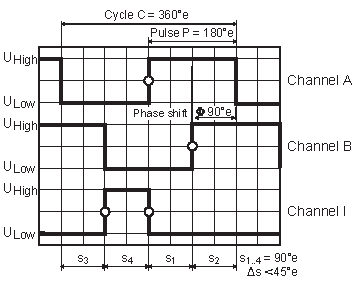
\includegraphics[width=0.5\columnwidth]{encoder.pdf}
	\caption{Encoder signal sensor states depending on position \cite{motor_encoder}.}
	\label{fig:encoder}
\end{figure}

\subsubsection{FPGA}

The FPGA built into the sbRIO is taking care of the interfacing between the controllers and the microprocessor. The code running on the FPGA is much faster than the one running on the microprocessor. To reach maximum possible speed, we implemented whatever we could on the FPGA, however the FPGA is incapable of handling higher level functions such as string handling and UDP networking.

The FPGA's main functions are the following:

\begin{itemize}	
	\setlength\itemsep{0em}
	\item Count the encoder ticks coming from the controller
	\item Read the controller's analog and digital inputs 
	\item Calculate position PID control signal and send the corresponding PWM signal to the controller
	\item Enable the motors
	
\end{itemize}

Since the current value coming from the ESCON is noisy, the FPGA also needs a built in low pass filter.

\subsubsection{ESCON motor controllers}
\label{escon_con}

The ESCON controllers are programmed to output a speed corresponding to the FPGA PWM signal. The speed controller has an inner current controller, which also keeps the motors from taking overcurrent. The current ramps can be adjusted to fit the user's needs. The speed control gain can be adjusted by the onboard potmeter. 
The outer speed loop provides the control signal for the internal current controller. The inner control loop must have a higher frequency than the speed control loop. The PI current controller is running at 53.6 kHz, while the PI speed controller is running at 5.36 kHz. The inner loop ensures fast response, the outer higher precision \cite{cascade_cont}. The advantages of the cascade structure:

\begin{itemize}
	\item Better setpoint tracking
	\item Better disturbance rejection
	\item Less delay and phase lag
\end{itemize}

The position is controlled by setting the duty ratio of the incoming PWM signal. The speed reference is 0 at 50\% duty ratio and grows linearily at higher values.
The ESCON controller has 2 programmable analog outputs, thus we are unable to read speed, actual current and demand current simultaneously.
The controllers have autocalibration functionalities, but this ability is obstructed by the gearing limits.

ESCON Studio provides the tool for logging data from the ESCON controller by using only a USB cable.